%%%%%%%%%%%%%%%%%%%%%%%%%%%%%%%%%%%%%%%%%
% Wenneker Article
% LaTeX Template
% Version 2.0 (28/2/17)
%
% This template was downloaded from:
% http://www.LaTeXTemplates.com
%
% Authors:
% Vel (vel@LaTeXTemplates.com)
% Frits Wenneker
%
% License:
% CC BY-NC-SA 3.0 (http://creativecommons.org/licenses/by-nc-sa/3.0/)
%
%%%%%%%%%%%%%%%%%%%%%%%%%%%%%%%%%%%%%%%%%

%----------------------------------------------------------------------------------------
%	PACKAGES AND OTHER DOCUMENT CONFIGURATIONS
%----------------------------------------------------------------------------------------

\documentclass[11pt, a4paper, onecolumn]{article} % 10pt font size (11 and 12 also possible), A4 paper (letterpaper for US letter) and two column layout (remove for one column)
\usepackage{textgreek}
\setlength{\parskip}{\baselineskip}
%\setlength{\parindent}{5pt}
%%%%%%%%%%%%%%%%%%%%%%%%%%%%%%%%%%%%%%%%%
% Wenneker Article
% Structure Specification File
% Version 1.0 (28/2/17)
%
% This file originates from:
% http://www.LaTeXTemplates.com
%
% Authors:
% Frits Wenneker
% Vel (vel@LaTeXTemplates.com)
%
% License:
% CC BY-NC-SA 3.0 (http://creativecommons.org/licenses/by-nc-sa/3.0/)
%
%%%%%%%%%%%%%%%%%%%%%%%%%%%%%%%%%%%%%%%%%

%----------------------------------------------------------------------------------------
%	PACKAGES AND OTHER DOCUMENT CONFIGURATIONS
%----------------------------------------------------------------------------------------

\usepackage[english]{babel} % English language hyphenation

\usepackage{microtype} % Better typography

\usepackage{amsmath,amsfonts,amsthm} % Math packages for equations

\usepackage[svgnames]{xcolor} % Enabling colors by their 'svgnames'

\usepackage[hang, small, labelfont=bf, up, textfont=it]{caption} % Custom captions under/above tables and figures

\usepackage{booktabs} % Horizontal rules in tables

\usepackage{lastpage} % Used to determine the number of pages in the document (for "Page X of Total")

\usepackage{graphicx} % Required for adding images

\usepackage{enumitem} % Required for customising lists
\setlist{noitemsep} % Remove spacing between bullet/numbered list elements

\usepackage{sectsty} % Enables custom section titles
\allsectionsfont{\usefont{OT1}{phv}{b}{n}} % Change the font of all section commands (Helvetica)

%----------------------------------------------------------------------------------------
%	MARGINS AND SPACING
%----------------------------------------------------------------------------------------

\usepackage{geometry} % Required for adjusting page dimensions

\geometry{
	top=1cm, % Top margin
	bottom=1.5cm, % Bottom margin
	left=2cm, % Left margin
	right=2cm, % Right margin
	includehead, % Include space for a header
	includefoot, % Include space for a footer
	%showframe, % Uncomment to show how the type block is set on the page
}

\setlength{\columnsep}{7mm} % Column separation width

%----------------------------------------------------------------------------------------
%	FONTS
%----------------------------------------------------------------------------------------

\usepackage[T1]{fontenc} % Output font encoding for international characters
\usepackage[utf8]{inputenc} % Required for inputting international characters

\usepackage{XCharter} % Use the XCharter font

%----------------------------------------------------------------------------------------
%	HEADERS AND FOOTERS
%----------------------------------------------------------------------------------------

\usepackage{fancyhdr} % Needed to define custom headers/footers
\pagestyle{fancy} % Enables the custom headers/footers

\renewcommand{\headrulewidth}{0.0pt} % No header rule
\renewcommand{\footrulewidth}{0.4pt} % Thin footer rule

\renewcommand{\sectionmark}[1]{\markboth{#1}{}} % Removes the section number from the header when \leftmark is used

%\nouppercase\leftmark % Add this to one of the lines below if you want a section title in the header/footer

% Headers
\lhead{} % Left header
\chead{\textit{\thetitle}} % Center header - currently printing the article title
\rhead{} % Right header

% Footers
\lfoot{} % Left footer
\cfoot{} % Center footer
\rfoot{\footnotesize Page \thepage\ of \pageref{LastPage}} % Right footer, "Page 1 of 2"

\fancypagestyle{firstpage}{ % Page style for the first page with the title
	\fancyhf{}
	\renewcommand{\footrulewidth}{0pt} % Suppress footer rule
}

%----------------------------------------------------------------------------------------
%	TITLE SECTION
%----------------------------------------------------------------------------------------

\newcommand{\authorstyle}[1]{{\large\usefont{OT1}{phv}{b}{n}\color{DarkRed}#1}} % Authors style (Helvetica)

\newcommand{\institution}[1]{{\footnotesize\usefont{OT1}{phv}{m}{sl}\color{Black}#1}} % Institutions style (Helvetica)

\usepackage{titling} % Allows custom title configuration

\newcommand{\HorRule}{\color{DarkGoldenrod}\rule{\linewidth}{1pt}} % Defines the gold horizontal rule around the title

\pretitle{
	\vspace{-30pt} % Move the entire title section up
	\HorRule\vspace{10pt} % Horizontal rule before the title
	\fontsize{32}{36}\usefont{OT1}{phv}{b}{n}\selectfont % Helvetica
	\color{DarkRed} % Text colour for the title and author(s)
}

\posttitle{\par\vskip 15pt} % Whitespace under the title

\preauthor{} % Anything that will appear before \author is printed

\postauthor{ % Anything that will appear after \author is printed
	\vspace{10pt} % Space before the rule
	\par\HorRule % Horizontal rule after the title
	\vspace{20pt} % Space after the title section
}

%----------------------------------------------------------------------------------------
%	ABSTRACT
%----------------------------------------------------------------------------------------

\usepackage{lettrine} % Package to accentuate the first letter of the text (lettrine)
\usepackage{fix-cm}	% Fixes the height of the lettrine

\newcommand{\initial}[1]{ % Defines the command and style for the lettrine
	\lettrine[lines=3,findent=4pt,nindent=0pt]{% Lettrine takes up 3 lines, the text to the right of it is indented 4pt and further indenting of lines 2+ is stopped
		\color{DarkGoldenrod}% Lettrine colour
		{#1}% The letter
	}{}%
}

\usepackage{xstring} % Required for string manipulation

\newcommand{\lettrineabstract}[1]{
	\StrLeft{#1}{1}[\firstletter] % Capture the first letter of the abstract for the lettrine
	\initial{\firstletter}\textbf{\StrGobbleLeft{#1}{1}} % Print the abstract with the first letter as a lettrine and the rest in bold
}

%----------------------------------------------------------------------------------------
%	BIBLIOGRAPHY
%----------------------------------------------------------------------------------------

\usepackage[backend=bibtex,style=authoryear,natbib=true]{biblatex} % Use the bibtex backend with the authoryear citation style (which resembles APA)

\addbibresource{noisewalls.bib} % The filename of the bibliography

\usepackage[autostyle=true]{csquotes} % Required to generate language-dependent quotes in the bibliography
 % Specifies the document structure and loads requires packages

%----------------------------------------------------------------------------------------
%	ARTICLE INFORMATION
%----------------------------------------------------------------------------------------


\title{Investigation of the SNR Wall on Conscious EEG Signals} % The article title

\author{
	\authorstyle{Bernd Porr\textsuperscript{1} and Nikolas Kyriacou\textsuperscript{2}} % Authors
	\newline\newline % Space before institutions
	\textsuperscript{1}\institution{Project Advisor}\\
	\textsuperscript{2}\institution{MSc Student}
}

% Example of a one line author/institution relationship
%\author{\newauthor{John Marston} \newinstitution{Universidad Nacional Autónoma de México, Mexico City, Mexico}}

%\date{\today} % Add a date here if you would like one to appear underneath the title block, use \today for the current date, leave empty for no date

%----------------------------------------------------------------------------------------

\begin{document}
%\frontmatter % Use roman page numbering style (i, ii, iii, iv...) for the pre-content pages
%
%\includegraphics[width=\textwidth]{Figures/Univ_Logo.jpg}
\maketitle % Print the title

\thispagestyle{firstpage} % Apply the page style for the first page (no headers and footers)





%----------------------------------------------------------------------------------------
%	ABSTRACT
%----------------------------------------------------------------------------------------

%\lettrineabstract{Lorem ipsum dolor sit amet, consectetur adipiscing elit. Fusce maximus nisi ligula. Morbi laoreet ex ligula, vitae lobortis purus mattis vel. Vestibulum ante ipsum primis in faucibus orci luctus et ultrices posuere cubilia Curae; Donec ac metus ut turpis mollis placerat et nec enim. Duis tristique nibh maximus faucibus facilisis. Praesent in consequat leo. Maecenas condimentum ex rhoncus, elementum diam vel, malesuada ante.}
\newpage
\begin{abstract}
Brain Computer Interfaces (BCI) are closed loop systems used to control the operation of devices such as a wheelchair, or a robot arm, as well as in games as the user interface. The ability of a BCI system in detecting correctly the user’s intent depends on parameters such as the classification algorithm, the number and position of EEG electrodes used and the frequency bands examined. The aim of this project is to investigate the ability of a BCI system to detect EEG signals, recorded with the use of a single electrode attached on the Fp1 position. The frequency band examined is the alpha band (8Hz to 12Hz) with more emphasis at the 10Hz peaks.


A number of experiments were devised to be conducted with the help of a number of willing persons acting as the subjects. This however, requires a prior approval by the Ethics Committee of the University. Because this approval was not granted on time, the signals used for the analysis of the EEG activity are taken from EEG recordings of the author of this report only. For the purpose of this project the conscious signal is considered to be the EEG signal recorded during the time that the subject is concentrating on the mental activity specified by the experiment. The EEG background noise is the EEG signal recorded when the subject is relaxed. The subject was instructed to avoid any movements that could create artefacts. 


The spectrum of the recorded signals was examined in order to investigate the behaviour of the 10Hz peaks. From the processed EEG signals it was verified that the 10Hz are indeed present, while the frequency of the peaks shifts slightly between 9Hz and 11Hz. Furthermore, it was observed that the power of these peaks varies according to the mental effort of the subject. The SNR of the recorded signals was then calculated and compared to threshold noise levels called the noise walls. The values of this SNR noise walls were computed in another project conducted 2018. The investigation of the SNR showed that the calculated SNR was higher than the “relax” and the “Sudoku” SNR walls, while It was lower for the “eye blinking” artefact, thus the investigated BCI system can detect the EEG signals, while care must be  taken in handling artefacts.

\end{abstract}

%----------------------------------------------------------------------------------------
%	ARTICLE CONTENTS
%----------------------------------------------------------------------------------------

\newpage
\section*{ACKNOWLEDGEMENTS}
I would like express my thanks and gratitude towards my project advisor Dr. Bernd Porr, for his guidance and assistance throughout the implementation of the work of this project. I found his views and suggestions on the subject incredibly interesting and useful. 
\newpage
\tableofcontents % Prints the main table of contents
\newpage
\listoffigures % Prints the list of figures

%\mainmatter % Begin numeric (1,2,3...) page numbering
\newpage
\section{\centerline{Introduction}}
\label{sec:introduction}

\vspace {15pt}
Electroencephalogram (EEG) is the recording of electrical signals from the scalp, representing the electrical activity of the brain. EEG is used for decades as a medical tool to diagnose brain diseases such as epilepsy, as well as a diagnostic test in psychiatry. EEG signals are also used in Brain Computer Interface (BCI) systems, most of which are based on motor imagery resulting in movement execution. Examples of BCI applications are the control of the operation of a wheelchair, or a robot arm, as well as in games as the user interface. In BCI systems, decisions are made based on consciously generated EEG signals by the user. BCI are closed loop systems, since the user observes the effect on the device to be controlled and in a way adjusts his brain activity accordingly. Through this process a user can become more effective in the control of a device through practice.  
 
EEG signals are subject to noise which in some cases has amplitude much greater than the amplitude of the desired EEG signal. For a successful BCI operation, this noise must be removed or avoided, since the noise can result in a false detection of the user’s intention. The ability of a BCI system to detect the user’s intent with a correct decision made depends also on other factors such as the number of electrodes used to record the EEG signals, the scalp positions they are placed, since different scalp positions are more suitable for detecting different brain activities, as well as on the EEG signal frequencies examined.
 
The purpose of this project is to investigate the capability of EEG signals in providing the necessary information for the detection of the user’s intention in BCI systems, when using a single electrode connected to the Fp1 position of the scalp. This investigation includes the recordings of EEG signals produced by willing persons, consciously performing a mental task such as trying to move an object on the screen of a computer, as well as the analysis of the power spectrum of the EEG signals in the alpha frequency band (8Hz to 12Hz) and the computation of the signal-to-noise ratio (SNR).   

\subsection{\bf{Noise in EEG signals:}}

The strength of EEG signals is very small, in the order of microvolts. EEG signals suffer from noise, which in some cases has amplitude much greater than the signal amplitude. This noise can be either due to the external noise generated by electrical devices, such as the 50Hz mains noise, or due to body muscular activity, known as the artefacts. Possible sources of artefacts, are activities from other parts of the body that generate electrical signals, such as the noise due to eye movement and eye blinking, heart activity and facial muscle movements  \citep{Yong2008}. Furthermore, EEG signals contain information on the conscious intent of the subject, as well as other signals due to brain activity not related to the specific intent of the subject. These other signals can also be treated as noise, since they affect the accuracy of decision making on the subject’s intent. This noise is usually called the background noise. In BCI conscious applications, in order to be able to analyse EEG signals correctly and obtain a successful decision, it is essential that noise is removed, or discard the recorded data for the duration during which the artefact is detected  \citep{Balbir2017,Repovs2010}. The option of discarding the EEG signal segments when noise is detected in not always possible. For example EEG background EEG is always present.  

In theory, the information from a noisy EEG signal can be correctly extracted, given that a minimum number of signal samples are used, or the signal is examine for a minimum time duration. This implies that as the SNR of the EEG signal decreases, the required number of samples or the signal duration must be increased. If the SNR becomes very low, then the number of required samples or the signal time duration becomes infinite. Therefore, there is a minimum limit of the SNR, beyond which the signal information cannot be correctly determined, called the SNR Wall \citep{Tandra2008a,Kustra2017,Tandra2008b}. A study on the SNR Wall in relation to the SNR of EEG signals has already been done at the University of Glasgow during the academic year 2017-2018 \citep{Porr2018}. This study included the development of the methodology and the mathematical equations needed to compute the SNR wall and the SNR for the recorded signals for various settings, such as eye blink, smile and reading aloud a text. In this work, the EEG and the electromyography (EMG) signals due to artefacts are considered as noise and the SNR calculations are done based on the energy of the artefact EEG/EMG signals. For the calculation of the SNR signal power is considered to be the conscious change in EEG power from paralyzed persons \citep{Whitham2007}.
    
\subsection{\bf{Project Aims and Objectives:}}
The aim of this project is to develop a methodology that enables the investigation of the capability of EEG signals in providing the necessary information for the detection of the user’s intention when using a single electrode connected to the Fp1 position of the scalp. More specifically, the objectives of this project are to:

\begin{enumerate}
	\item Produce a literature review on the main issues related to the work of the project. This review will concentrate on motor imagery BCI systems.
	\item	Setup and configure a BCI hardware consisting of an EEG signal amplifier and a 24-bit sigma-delta A/D converter board. This hardware is based on existing boards available by the University of Glasgow. 
	\item	Devise experimental settings and perform a number of experiments that will enable the recording of EEG signals from a number of persons who will consciously try to perform a brain function, such as trying to move an object on the screen of a computer, or attempting to increase their own 10Hz peak in their EEG spectrum. 
	\item	Devise the methodology and build the necessary software that will enable the analysis of the conscious EEG signals recorded.
	\item	Analyse the recorded EEG with respect to their SNR characteristics, in order to determine whether EEG signals in the alpha frequency zone, obtained from a single electrode connected to Fp1 position on the scalp can be safely used by BCI systems to determine the intent of a user. 
\end{enumerate}

\subsection{\bf{Project Methodology:}}
For the purpose of this project, the analysis of the EEG signals and the estimation of the intent of the person will be based on the time domain and the frequency spectrum of the EEG signals. Earlier research work has shown a relationship between the person’s intent and the frequency band of the EEG signals \citep{Wolpaw1991,Wolpaw2004}. Other parameters that could affect the analysis of the EEG signals, are the number of electrodes (sensors) used and the scalp position of the electrodes. This project examines the EEG signals in the alpha frequency band (8Hz to 12Hz) taken from an electrode connected to the Fp1 position. This emulates a typical EEG gadget for gaming control.

To investigate the EEG signals in the alpha wave frequency band taken from an electrode connected to the Fp1 position and the achieved SNR, experiments were done with a person referred to as the subject. The experiments were conducted with a data acquisition system consisting of the EEG electrodes, a custom made signal amplifier with a voltage gain of 50, and the “USB DUX SIGMA” 24-bit analogue-to-digital converter board (Porr, B linux-usb-daq.co.uk). EEG recordings were made using the open source software “Comedirecord” (Porr B. , ComediRecord). This software enables the acquisition of signals, signal filtering, display of time domain signal, display of the frequency spectrum and the recording of the raw signal.
 
 During the experiment’s procedure, the subject was performing a mental task, such as trying to move an object on screen of a computer, while at the same time observing the 10Hz peak of the real time spectrum of the generated EEG signal on the screen of the computer. The EEG signals generated by the subject were recorded on a computer. This enables a closed loop control of the BCI system. The subjects were looking at their own Fourier spectrum and trying to consciously maximize the alpha band frequency peak, thus achieving maximum SNR.

The recorded EEG signals were filtered to remove any external noise, such as the 50Hz mains noise. To isolate the alpha band frequencies, the EEG recordings were also filtered by a bandpass filter. The SNR wall was calculated for each subject using as noise signal the first part of the recording of each experiment for the specific subject. This part of the signal corresponds to the time period that the subject is relaxed. This calculation was achieved using the maximum and the minimum variances between the recordings of the different experiments. The calculation of the SNR was based on the information signal which is the EEG signal during the instances that a person is consciously performing a mental operation, while the noise was the background EEG noise signal obtained when the person was relaxed, doing nothing. For each experiment, the SNR was compared to the SNR wall in order to specify whether a detection can be made or not. The power of the EEG signal related to the intent of the subject was varying during the time of the effort of the subject. For this reason, the SNR was calculated for signal segments corresponding to one-second time periods, with a 500ms time difference between adjacent signal segments. The proposed methodology can help in identifying the instance during which the SNR is maximum and therefore, use this EEG signal segment for the decision on the subject’s intent.

The subjects were instructed to avoid any intentional movements that could create artefacts. In the case that artefacts ware identified in the EEG recordings, the signal segment corresponding to the duration of the artefact was ignored.
   
\subsection{\bf{Background Theory:}}
Electroencephalography (EEG) refers to the recordings of the electrical activity of the brain. The origins of EEG dates back in 1875 when Richard Caton observed EEG signal activity in exposed brains of animals. The first EEG recordings in humans were reported by Hans Berger in 1924. EEG has evolved since then and is currently used in clinical applications to detect coma and brain death, to locate brain areas damaged after head injury or stroke, to control anesthesia depth, to investigate epilepsy and seizure, to investigate sleep disorders and many other applications. EEG is also the means of providing information on the user’s intent in Brain Computer Interfaces (BCI) used to control the operation of actuators in devices such as wheelchairs and human prosthetic limbs, as well as in gaming. 

\subsubsection{\bf{EEG Signals:}}
EEG signals are electrical signals representing brain activity. When EEG signals are obtained through specialized electrodes attached on the scalp, the process used is referred to as non-invasive. Due to the fact that in non-invasive EEG the electrical signals are taken from the scalp, EEG signals are weak, in the order of microvolts (µV). To improve the quality of the recorded EEG signals the electrodes are placed on the scalp using a conductive gel. Furthermore, the scalp area is prepared with a light abrasion to remove dead skin cells and thus reduce the scalp impedance. In many systems the electrodes are embedded on caps or nets. 
Information deduced from EEG signals depends on the scalp position where the electrodes are attached. This is due to the fact that different parts of the brain are related to different brain activities. Therefore, mapping schemes are used to identify the scalp positions where electrodes can be attached. A common mapping scheme widely used is the “International 10-20” scheme \citep{Towle1993}, shown in Figure \ref{I20map}. 


\begin{figure}
	\centering
%	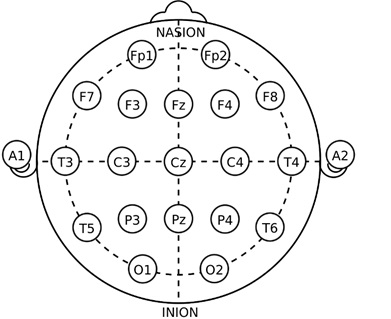
\includegraphics[width=\linewidth]{Figures/Brain_I20.jpg} % Figure image
	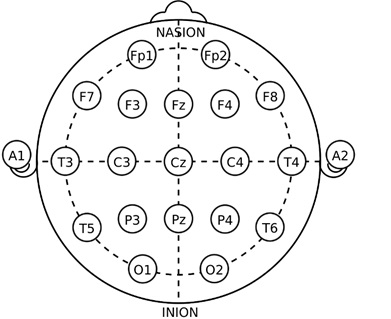
\includegraphics[width=8cm]{Figures/Brain_I20.jpg} % Figure image
	\caption{The International 10-20 mapping} % Figure caption
	\label{I20map} % Label for referencing with \ref{bear}
\end{figure}

% \begin{enumerate}[label=\alph*.] \item Blablah 1 \item Blablah 2 \item Blablah 3 ...


Another factor that relates to the information conveyed by EEG signals is the EEG rhythmic activity, identified in different frequency bands \citep{Fink2014}. These frequency bands are the following:

\begin{enumerate} [label=\alph*)]
	\item Delta (<4Hz) 
	\item Theta (4Hz to 7Hz)
	\item Alpha (8Hz to 12Hz) 
	\item Beta (12Hz to 30Hz)
	\item Gamma (>31Hz)
	\item Mu (8Hz to 12Hz)  
\end{enumerate} 

The Alpha frequency band is also referred to occupy the frequency range from 8Hz to 15Hz in bibliography. The Mu frequency band overlaps with the alpha frequency band and refers to the EEG signals taken from the motor cortex (C3, Cz, and C4 electrode positions).  

Decoding brain activity is a function of both the frequency band examined and the electrode positions used to record the EEG signals. When performing a motor task, or imagine of a motor task the energy from the mu (alpha) and the beta rhythms will rise or fall. Event related synchronization (ERS) refers to the case when the energy rises, while event related desynchronization (ERD) refers to the case when the energy falls. ERD in the mu band is observed during the performance of a motor task. This is known as the mu suppression. ERD occurs also by observing a motor action carried out by another person. A study of the mu suppression on different areas of the alpha band frequency (8Hz to 10Hz and 10Hz to 12Hz) prior and during hand/foot movements showed a higher mu suppression in the lower frequencies \citep{Pfurtscheller2000}.  A study in \citep{Khulman1978} showed that manual execution resulted in a maximum ERD at the frequency of 10.1Hz. The effect in ERD when performing and observing manual movements with respect to frequency ranges in the alpha frequency band and the spatial domains is examined in \citep{Frenkel2013}. The effect of ERD when performing or observing hand movements is shown in Figure \ref{Scalp}. 


\begin{figure}
	\centering
	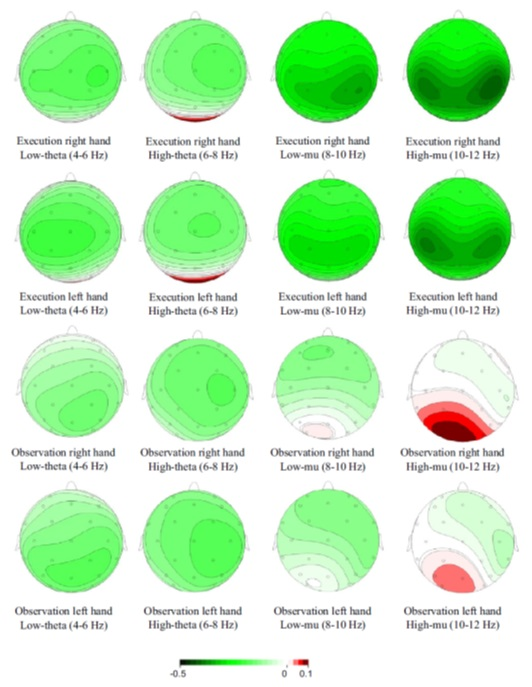
\includegraphics[width=\linewidth]{Figures/ScalpSignals.jpg} % Figure image
%	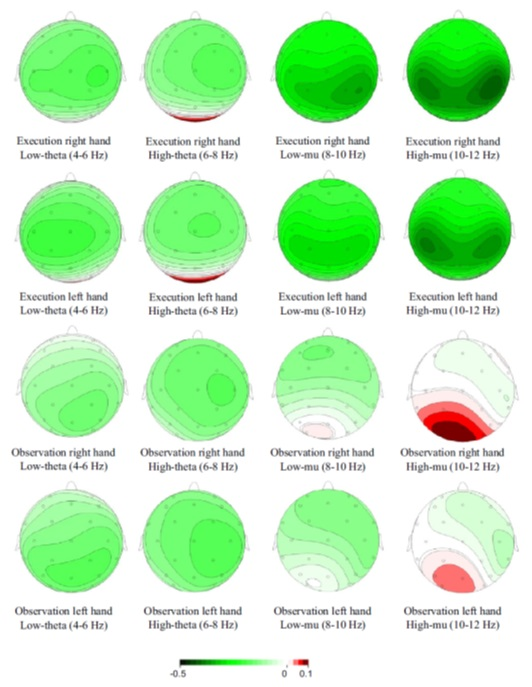
\includegraphics[width=14cm]{Figures/ScalpSignals.jpg} % Figure image
	\caption{The scalp distribution of suppression in the different execution and observation conditions. (Figure taken from \citep{Frenkel2013}.} 
	\label{Scalp} % Label for referencing with \ref{bear}
\end{figure}


\subsubsection{\bf{Noise in EEG Signals:}}
EEG signals are contaminated by noise. EEG noise is considered to be any EEG electrical signal recorded that is the signal amplifier is place not produced by brain activity. This noise can be externally produced by external sources such as electrical or electronic devices, or produced by the movements of the electrode assembly. Another source of noise in EEG is the noise due to the operation and activities of the human body, such as smiling or eye movement, referred to as the artefacts. In the study and decoding of EEG recordings, signals due to brain activity not related to the activity examined are often assumed and treated as noise.    

\subsubsection{\bf{External Noise:}}

External noise in EEG signal recordings is primarily due to the operation of electrical or electronic equipment operating in the area of the recording. The frequency range of this noise can range from low frequencies in the range of frequencies related to EEG signals, to higher frequencies according to the type of the electronic device. The primary source of external noise is the 50Hz noise from the mains. This noise can be easily removed from the EEG signal using notch filters. To reduce the noise due to the operation of electronic devices, it is essential to perform the recording in a room where electronic devices such as mobile devices are removed. Some researchers use battery operated laptops instead of desktops for the recordings, in order to eliminate the 50Hz noise. 
A second source of external noise is the noise created by the electrode assembly system itself. This noise can be created by the movement of the cables connecting the electrodes with the amplifier, by misplaced electrodes or by badly connected grounding electrodes. This noise can have components in any frequency and is difficult to identify. To reduce this noise as much as possible it is essential that the electrode wires are short, the signal amplifier is placed as close as possible to the head and the electrodes are firmly attached with the use of a cap. Finally, the impedance between the electrode and the skin must be as small as possible. This can be ensured by the use of high quality electrodes, the use of a special gel and by cleaning the point of contact between the electrode and the skin.     
 
\subsubsection{\bf{Artefacts:}}
Artefacts are electrical signals recorded with EEG signals which are not due to the brain activity. Some of the common sources of artefacts are: 
\begin{enumerate} [label=\alph*)]
	\item Eye-induced artefacts: This includes eye blinking, eye movement, and movements of the extraocular muscles. The power spectrum of the eye-induced artefacts is concentrated in the 0.5Hz to 3Hz range and it is much higher than the normal EEG power. Higher frequency bands, such as the alpha band (8Hz to 12Hz) are also contaminated by eye-induced artefacts \citep{Manoilov2006, Tamburro2018}. 
	\item Muscle activation-induced artefacts: This incudes primarily noise due to the activity of facial muscles such as smiling or chewing \citep{Yong2008}. The power spectrum of this artefact covers the whole of the frequency range of EEG signals, with higher values observed at frequencies below 20Hz \citep{Tamburro2018}.        
	\item Cardiac artefacts: This artefacts are due to heart activity. The power spectrum of the cardiac artefact has a peak at the frequency corresponding to the heart beat-rate (0.8Hz to 1.7Hz), with lower power values at frequencies up to 10Hz \citep{Tamburro2018}. 
\end{enumerate} 

The amplitude of artefacts is quite large compared to the amplitude of the brain activity related EEG signals of interest. In order to be able to analyse EEG signals correctly, it is essential that noise is removed from the EEG signals \citep{Balbir2017, Fitzgibbon2007, Mantini2008, Delorme2007}.  In cases where the artefact is temporal, such as the noise due to eye blinking, instead of removing the noise another option is to discard the recorded data for the duration during which the artefact is detected \citep{Repovs2010, Jirayucharoensak2013, Mognon2011}.

\subsubsection{\bf{Signal-to-Noise Ratio and SNR Walls:}}
A measure of the strength of the useful signal relative to the background noise is characterized by the signal-to-noise ratio. Since noise is unwanted signal that contaminates the useful signal, it is required to achieve a SNR value as high as possible in order to get a correct decision. As the noise level relative to the signal level increases, the SNR decreases, the quality of the signal decreases and the probability of extracting useful information from the signal is reduced. If the SNR drops below a given threshold, then it becomes impossible to extract any information from the signal.    
   
Stationary noise refers to the noise that has a level within a given range, where the limits of this range do not change with time. An example of stationary noise is the white noise. If the noise levels change significantly with time, then this noise is called a non-stationary noise. EEG noise due to artefacts is a non-stationary noise, since it depends on the activity of the person generating the EEG signals. 

A threshold of the minimum limit of the SNR, beyond which the signal information cannot be correctly determined, is called the SNR Wall \citep{Tandra2008a, Kustra2017, Tandra2008b}.  The investigation on the existence of the SNR Wall was based on a study on spectrum sensing concerning the possibility that a signal with an adequate power is present or not. Within this formula, the SNR Wall is defined as the “SNR below which robust detection is impossible for the given detector”. An alternative view of the SNR Wall relates to the sample complexity, or on the number of observations required to achieve a reliable detection.  In this sense, the SNR Wall states that “as the SNR approaches the SNR Wall, this sample complexity goes to infinity”. This implies that as the SNR of an EEG signal decreases, the required number of samples or the signal duration must be increased to ensure reliable signal detection. If the SNR becomes very low, then the number of required samples or the signal time duration becomes infinite. 

\subsubsection{\bf{Brain Computer Interfaces (BCI):}}
With the improvements in VLSI technology expressed in computers, microprocessors and analogue data converters, new applications, other than clinical diagnostics, have become a reality in recent years \citep{Liao2014, Ahmadi2012}. Brain Computer Interface (BCI) systems, use information from EEG signals to determine the intent of the BCI user \citep{Rak2012, Liu2018}. BCI applications include:

\begin{itemize}
	\item medical diagnostics \citep{Chung2015}, 
	\item prosthetic device control such as a robotic hand or arm, 
	\item assistive mobility such as the control of the operation of a wheelchair \citep{Gala2008}, or the control of the operation of a vehicle \citep{Babu2017},
	\item the movement of an object on the screen of a computer \citep{Wolpaw2004}, 
	\item EEG BCI games and virtual reality \citep{Martisius2016, Kerous2018, Ahn2014}. 
\end{itemize}

BCI systems rely on EEG signals consciously generated by the user in order to make decisions on the intent of the user and decide on the appropriate commands to be given to the device under control. The flow diagram of the operation of a typical BCI is shown in Figure  \ref{BCI_F}. The brain activity is recorded using the EEG recording system (electrodes, amplifier and data converter), the recorded EEG signal is then pre-processed to filter out any noise, then the features of interest are extracted from the filtered EEG signal, then a classification is made to decode the intent of the user and finally the necessary commands are given to the device controlled by the BCI system. BCI are closed loop systems, since the user observes the effect on the device to be controlled and, in a way adjusts his brain activity accordingly. Through this process a user can become more effective in the control of a device through practice.  

\begin{figure}
	\centering
	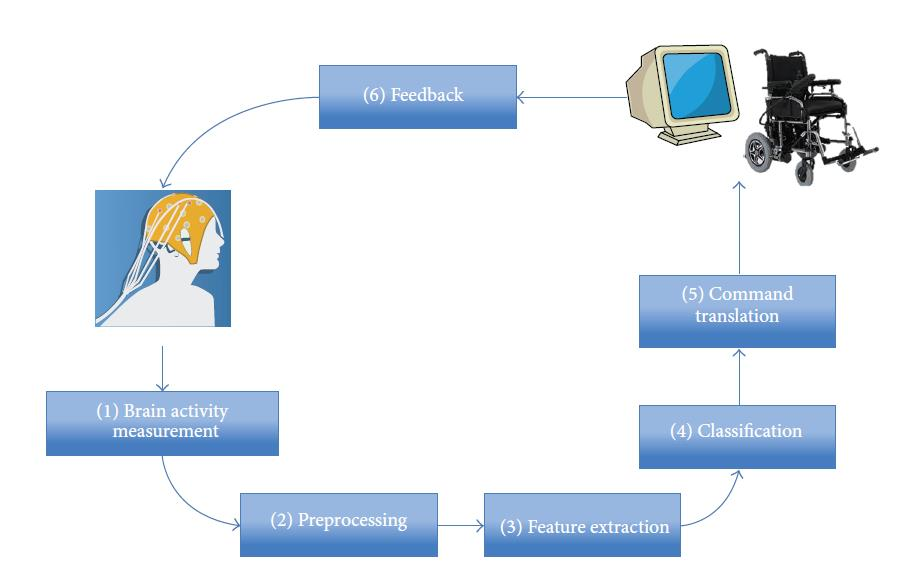
\includegraphics[width=\linewidth]{Figures/BCI_Flow.jpg} % Figure image
%	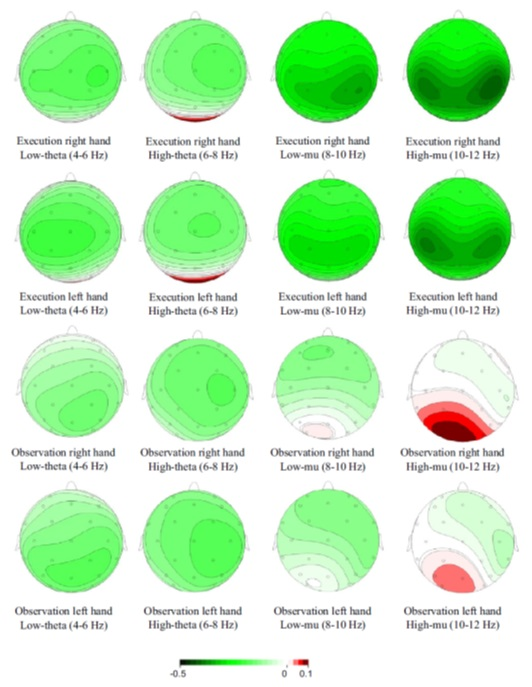
\includegraphics[width=14cm]{Figures/ScalpSignals.jpg} % Figure image
	\caption{Flow diagram of the operation of a typical BCI. (Figure taken from \citep{Martisius2016}.) }
	\label{BCI_F} % Label for referencing with \ref{bear}
\end{figure}

Currently, there are two main methods used in BCI for the feature extraction and classification. These are the Evoked Potentials (EP) and the Oscillatory or Motor Imagery EEG. 

\subsubsection{\bf{Evoked Potentials (EP):}}
Evoked Potential (EP) refers to techniques used to determine the brain activity after an external stimulus. There are two broad techniques of EP used in BCI. These are the Event Related Potentials (ERP) and the Visually Evoked Potentials (VEP).

\vspace {15pt}
\textbf{Event Related Potentials (ERP):}

In an ERP system, the brain response is examined after an external stimulus event. This response is a direct result of the stimulus. ERPs are very small compared to the background EEG activity, therefore, it is needed to average multiple ERPs to extract a clean ERP waveform \citep{Sanei2007}. ERP waveforms are characterized by a number of positive (P) peaks and negative (N) peaks and a number identifying the typical latency of the peak in ms or 100ms. A common ERP BCI system is the P300, which is based on the positive P3 part of the ERP waveform. The P300 BCI system is very common in EEG games \citep{Kerous2018}. A typical ERP waveform is shown in Figure \ref{ERP_F}. The negative voltages in ERP waveforms are usually shown on the upper part of the waveform.

\begin{figure}
	\centering
%	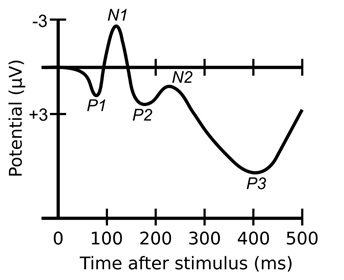
\includegraphics[width=\linewidth]{Figures/ERP.jpg} % Figure image
	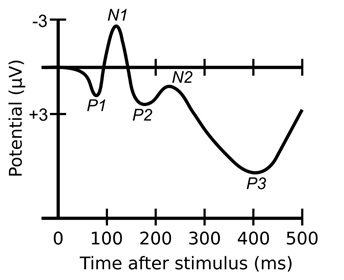
\includegraphics[width=10cm]{Figures/ERP.jpg} % Figure image
	\caption{A typical ERP waveform. (Figure taken from  \citep{Sanei2007}.) }
	\label{ERP_F} % Label for referencing with \ref{bear}
\end{figure}

EEG signals due to background brain activities, as well as artefacts and external signals are considered as noise with white noise characteristics. ERP signals are very weak compared to the rest of the recorded EEG signals, resulting in a low SNR. Therefore, to be able to interpret the ERP signal correctly it is necessary to increase the SNR. This is achieved by repeated trials and averaging the ERP signal. This is true given that the latency and shape of the ERP waveform does not change between trials and that the noise behaves as a zero-mean Gaussian noise.


\vspace {15pt}
\textbf{Visually Evoked Potentials (VEP):}

Visually Evoked Potentials (VEP) share the same characteristics with ERP, in the sense that both require averaging the EEG signals that are time-locked to a stimulus. The stimulus in this case is a light or a visual source. VEP is mainly used in ophthalmology.  

\subsubsection{\bf{Oscillatory or Motor Imagery (MI) EEG:}}
Motor Imagery (MI) BCI refers to BCI systems where motor imagery task being carried out are expressed as changes in the mu (alpha) and the beta frequency bands. When a mental activity results in an increase in a frequency band, this is called event-related synchronization (ERS). On the other hand, if the mental activity results in a decrease in a frequency band, then this is called event-related desynchronization (ERD).  MI BCI are widely used in medical applications, as well as in EEG games. 
Medical applications of MI BCI cover a wide range. Typical applications are, for example, the assistance in the rehabilitation of stroke patients using MI assisted with robotic feedback  \citep{Kai2010}. Another application is the use of MI BCI to control the operation of a wheelchair  \citep{Gala2008}.
The main function in an MI BCI is the classification of the imagery task, that is, the method that will enable the BCI identify the motor imagery task. A variety of methods are being used in order to determine the imagery task ranging from the analysis of the ERS/ERD activity in relation to the frequency band and the electrode positions used to record the EEG signal  \citep{Wolpaw2004, Pfurtscheller2006}, to artificial intelligence techniques, such as machine learning and fuzzy systems  \citep{Xu2009}. Furthermore, since classification requires the analysis of EEG signals recorded from different scalp areas with their spectrum changing with time, digital signal processing tools, such as the wavelet transforms  \citep{Ahmadi2012} are being used.  

\subsubsection{\bf{EEG based Games:}}
In recent years, the developments in smart and mobile devices, as well the success of BCI research in detecting correctly brain activity, resulted in the creation of a new sector in computer game technology. As noted in a review paper \citep{Ahn2014}, BCI games is a rapidly growing field used by healthy people, while there is a tremendous increase in the production of BCI related research papers, due to the availability of a variety of BCI game low price equipment. Some of the main manufactures of BCI game equipment are “Neurosky Mindset” (www.neurosky.com) and “Emotiv EPOC” (www.emotiv.com).  The complexity of the available BCI game equipment ranges from simple 1-electrode/sensor headsets to more complex devices with more than 16 electrodes/sensors. The control paradigms employed in implemented BCI games are the ERP/P300, the Motor Imagery and the Steady State Visual Evoked Potential (SSVEP).




%\begin{table}
%\caption{The effects of treatments X and Y on the four groups studied.}
%\label{tab:treatments}
%\centering
%\begin{tabular}{l l l}
%\toprule
%\tabhead{Groups} & \tabhead{Treatment X} & \tabhead{Treatment Y} \\
%\midrule
%1 & 0.2 & 0.8\\
%2 & 0.17 & 0.7\\
%3 & 0.24 & 0.75\\
%4 & 0.68 & 0.3\\
%\bottomrule\\
%\end{tabular}
%\end{table}


















%DDM model as well as detailed description
%of the DDM-CMP implementation and estimated performance results. The experimental 
%results show that, for the workload tested, the DDM-CMP architecture is able to achieve
%higher speedup values at lower power consumption levels comparing to traditional
%architectures. 

%While our previous work focused on the DDM model [2,3,12] and more recently on high-level %issues of DDM-CMP [5,6], such as estimations of the performance and power benefits, in this %paper we go a step further and present an analysis of the hardware budget for the DDM-CMP. As %a result we can now accurately determine the number of cores that may be included in a chip %with the same hardware budget as other traditional CPUs. In this paper we show that, in the %same hardware budget of a modern high-end single-chip microprocessor, it is possible to build %a DDM-CMP chip with 16 cores. The extra hardware cost for supporting execution under the DDM %model are shown to be less than 17\% of the total area. Moreover, we present and validate the %Runtime Support System of DDM-CMP. A careful design of this system allows the execution of %both regular and DDM applications without any modification to the CPU or the OS. This system %was validated using a functional Simics-based~\cite{simics} full system simulator.

%The rest of this paper is organized as follows. Section~\ref{sec:dataflow} presents 



\newpage
\section{\centerline{Related Work}}
\label{sec:related}


\vspace {15pt}
\subsection{\bf{Cursor Control by Wolpaw et. al.:}} 
The authors in the work in \citep{Wolpaw1991} present a one-dimensional cursor movement BCI, where the EEG were recorded from the scalp at the central sulcus. The task of the subjects was to move vertically a cursor from the centre of a video screen either upwards or downwards. The detection of the subjects’ intent was based on the EEG signals in the mu frequency band.  The work presented in \citep{Wolpaw2004} is a continuation of the work in \citep{Wolpaw1991}. 

The objective of this work was to show that the use of non-invasive BCI can assist people with spinal cord injuries by providing them the capability of real time multidimensional point to point movement control. This study was done with four human subjects, two with disabilities and two with no disabilities, and varying prior experience in using BCI technology. The task of the subjects was to move a cursor appearing in the centre of a computer screen to a target position, place at the edges of the screen. The control of the cursor movement was achieved by examining the amplitudes in the mu and the beta rhythm frequency bands in relation to the EEG signal recorded form the sensorimotor cortex (C3 and C4). Vertical movement control is based on the amplitudes of the C3 and C4 signals at the frequency of 24Hz.  Horizontal movement control is based on the amplitudes of the C3 and C4 signals at the frequency of 12Hz. The results obtained, with respect to the movement time, precision and accuracy are comparable to invasive BCI methods.

\subsection{\bf{The Mu (De)synchronization by Pfurtscheller et. al.:}}

The aim of this work \citep{Pfurtscheller2006} was to examine the effect of the imagination of the hands, foot and tongue movement with the EEG mu frequency band. This study was done with nine able-bodied subjects using 60 EEG electrodes. Through various trials, the effect on specific frequencies in the mu band was characterised with respect to the desynchronization and synchronization observed. The significance of this work was on the conclusion that event related desynchronization (ERD) and event-related synchronization can be used in BCI operated by motor imagery.


\subsection{\bf{A Hybrid BCI System Based on MI and Eye-Blinking by Liu et al.:} }
In this work \citep{Liu2018} the authors propose a hybrid BCI based on motor imagery with the aim to solve the problem of identifying the time at which the concious brain activity starts and ends. The proposed hybrid BCI combines an EEG recording system with an EOG system that provides the activity triggering signals by the state and position of the eyes of the subject. The start of the MI activity is signaled by the used by blinking his eyes. This triggers the EEG system to analyse and determine the intent of the user. In a similar way the user marks the end of the MI activity. 

This hybrid BCI system was tested with a 16 electrode data acquisition system. The task of the subject performing the evaluation experiments was to move a cursor at the screen of a computer following a predifined path. The decision on the subjects motor imagery command was determined according to the changes of the energy levels at the mu and the beta rhythm taken from the cerebral cortex positions.   


\subsection{\bf{BCI for Vehicle Navigation by Babu et. al.:}}
The work presented by the authors in \citep{Babu2017} is similar to the work presented in \citep{Liu2018} above, in the sense that they both use eye blinking to mark the beginning and the end of the motor imagery process. This is achieved by two EEG electrodes attached on the Fp1 and the Fp2 positions to identify eye blinking to mark the beginning or the end of the movement. The proposed BCI is used for the control of the movement of a vehicle. The motor imagery for the navigation of the vehicles is obtained through two electrodes connected on the C3 and C4 positions. The signals used for the control of the direction of the movement are in the mu band. The imagine direction of the movement is determined according to the power of the signals from the C3 and C4 electrodes.


\newpage
\section{\centerline{Methodology}}
\label{sec:methodology}


\vspace {15pt}
The aim of this project is to investigate the capability of EEG signals in providing reliable information for the detection of the user’s intent, when using a single electrode connected to the Fp1 position of the scalp. To achieve this experimentally, it is necessary to (a) setup the necessary equipment to facilitate the recordings of the EEG signals, (b) device the experiments that will enable the collection of appropriate data and (c) to specify the methodology to analyse the collected signals in order to complete the investigation and reach to a conclusion. An overview of the methodology to be used is shown in Figure \ref{overview}. As shown in Figure  \ref{overview}, the first part of the methodology concerns a closed loop BCI system where the EEG signals are amplified, sampled and stored in a computer file, while the spectrum of the EEG signal is displayed on the screen. The subject observes the spectrum and use it as a feedback of the effect of his/her effort. The second part concerns the analysis of the recorded EEG signal. This includes the pre-processing of the signal, the investigation on the effect of the spectrum of the alpha band frequencies and the calculation of the SNR. 

\begin{figure}[hbt!]
	\centering
	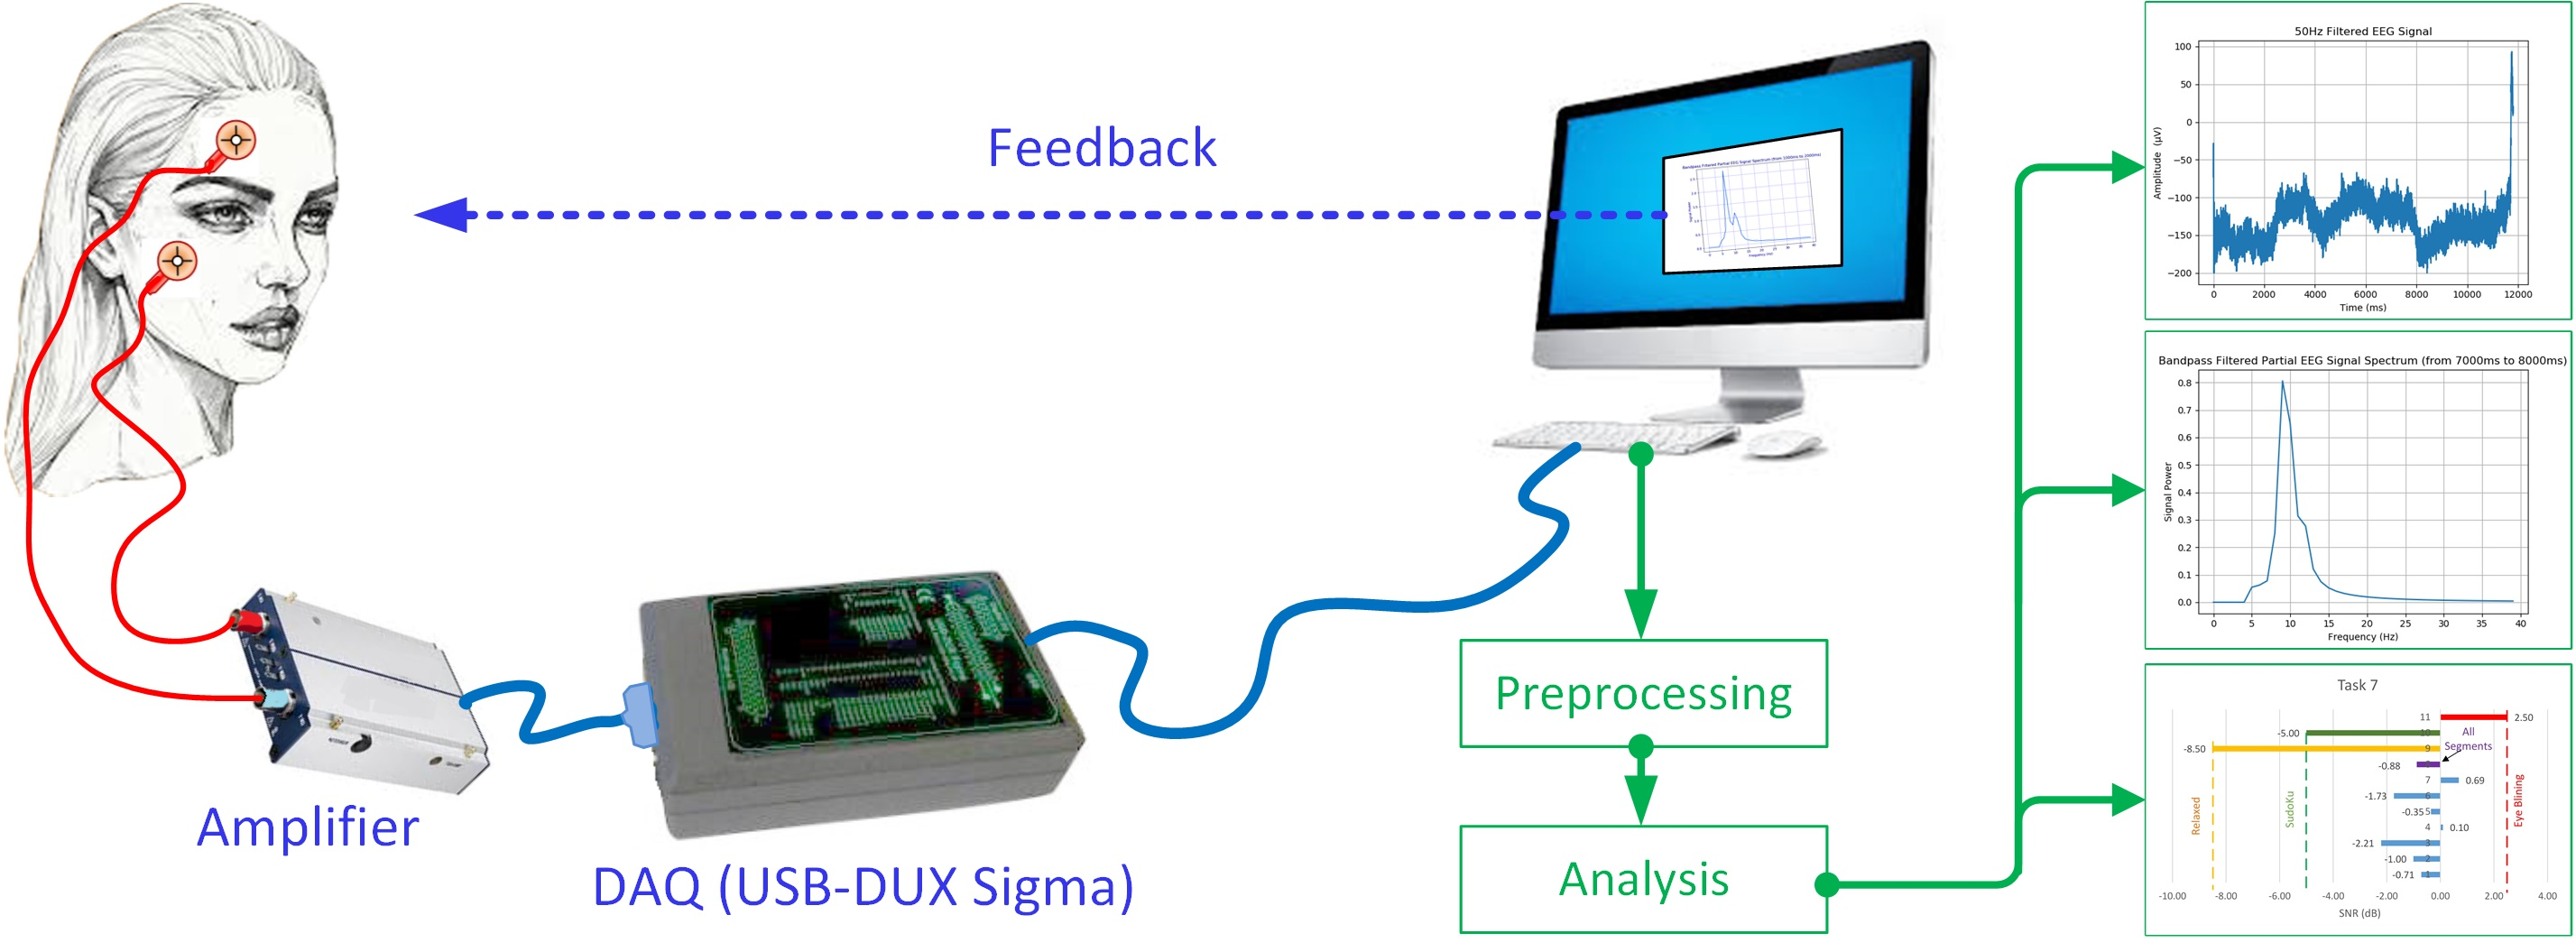
\includegraphics[width=\linewidth]{Figures/Overview.jpg} 
%	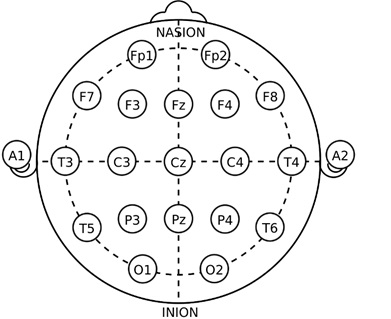
\includegraphics[width=8cm]{Figures/Brain_I20.jpg} 
	\caption{Methodology Overview} 
	\label{overview} 
\end{figure}

\subsection{\bf{Experimental Setup:}}
The hardware needed for the recording of EEG signals includes the EEG electrodes, the signal amplifier, the data acquisition hardware (Data converter board) and a computer. The diagram for the experimental setup is shown in Figure \ref{Hsetup}.

\begin{figure}[hbt!]
	\centering
	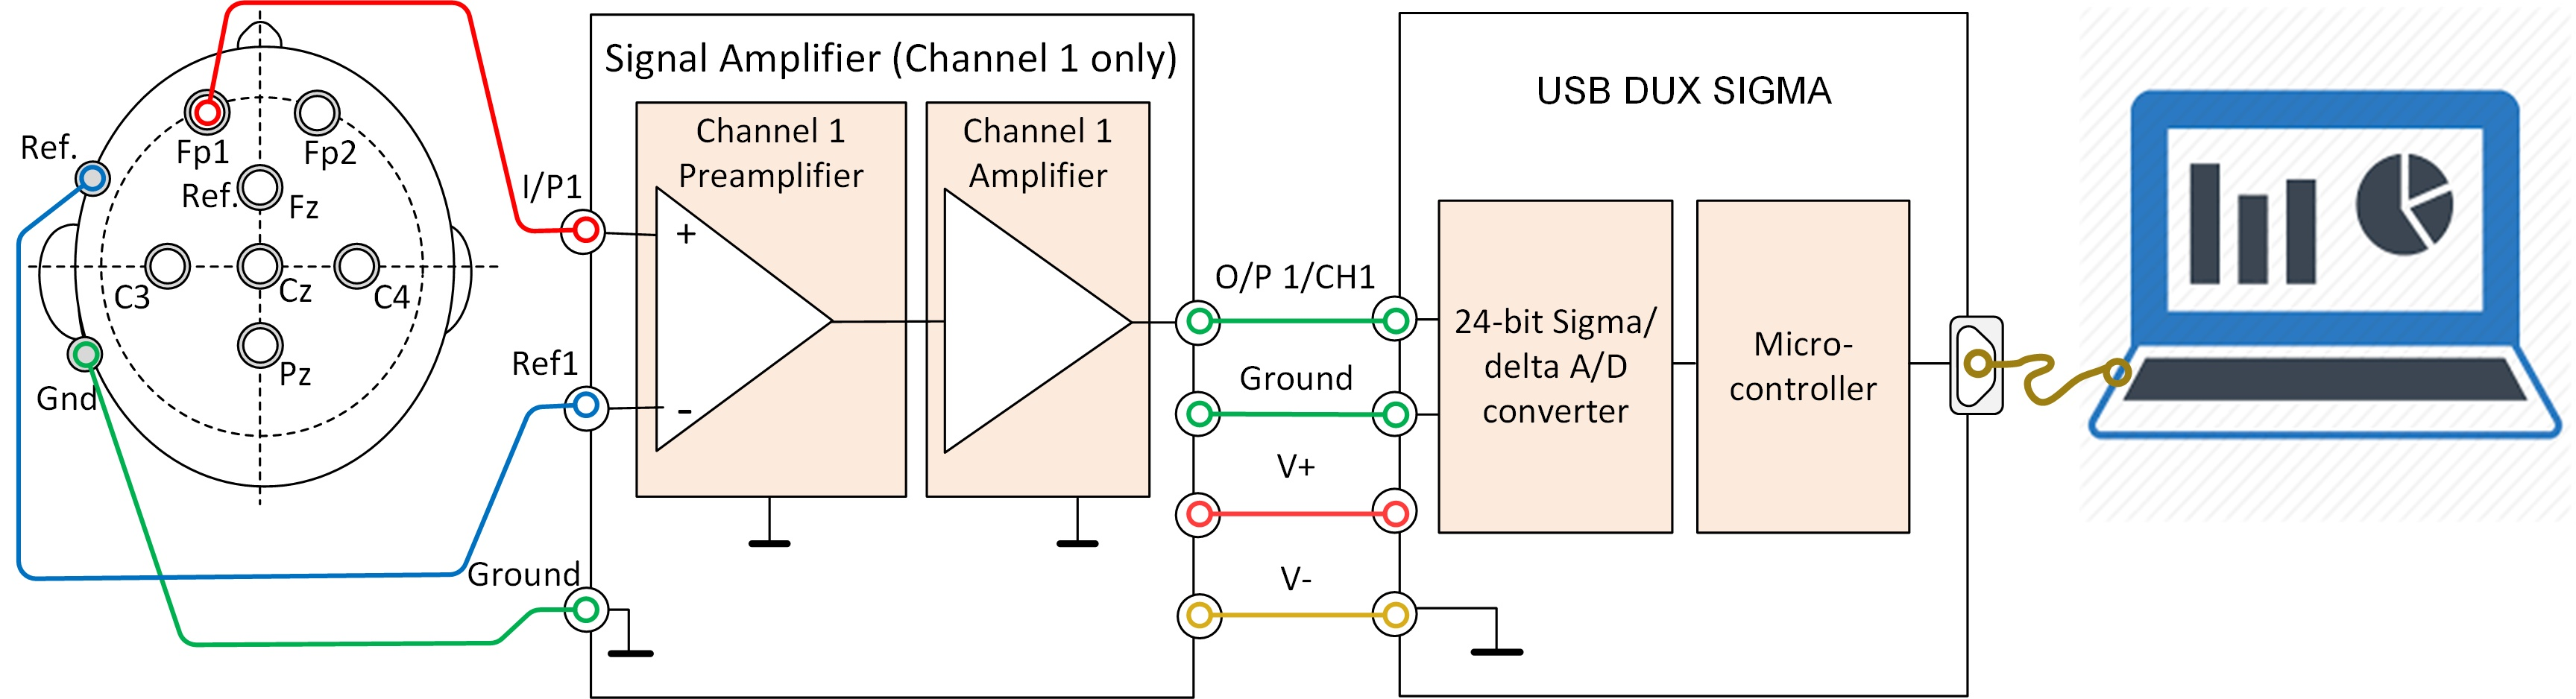
\includegraphics[width=\linewidth]{Figures/HardwareSetup.jpg} 
%	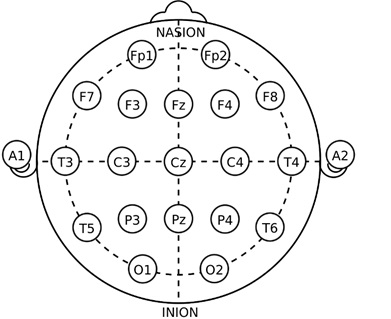
\includegraphics[width=8cm]{Figures/Brain_I20.jpg} 
	\caption{Block Diagram of the Experimental Setup} 
	\label{Hsetup} 
\end{figure}

Three disposable EEG electrodes are attached on the skin at the subject’s head area. The signal electrode is attached on the Fp1 position, the reference electrode is attached on the cheek and the ground is attached on the back of the ear of the subject. The EGG electrodes are kept in place by means of a hat that has the functionality of an EEG cap. 

The EEG signals are amplified by a custom made amplifier. This is a two-channel amplifier. The experiments were conducted using only one of the two channels. The gain of the amplifier is specified by two internal resistances and is set to be equal to 50. The voltage swing of the amplifier is from -5V to +5V. The signal amplifier is attached on a hat placed on the head of the subject. 

The output of the amplifier is connected to one of the analogue input channels of the data acquisition unit. This used is the “USB DUX SIGMA” 24-bit analogue-to-digital converter board (Porr, and linux-usb-daq.co.uk). This board has 16 analogue input channels with a maximum input voltage swing of -1.33V to +1.33V. The sampling frequency is 1KHz. Care must be taken in order not to exceed the maximum input voltage swing, because in such a case, the input signal will be clipped and behave like a square waveform with higher frequency harmonics.  The data acquisition unit provides also the supply voltage for the signal amplifier. The data acquisition unit is connected to a host computer through a USB cable. 

EEG recordings were made using the open source software “Comedirecord” \citep{Porr}. This software enables the acquisition of signals, signal filtering, display of time domain signal, display of the frequency spectrum and the recording of the raw signal.

\subsection{\bf{Experiment Procedure:}}
To investigate the EEG signals in the alpha wave frequency band taken from an electrode connected to the Fp1 position and the achieved SNR, experiments are required to be done with willing participants referred to as the subjects. During these experiments the subjects will be asked to perform a mental task. The EEG signals generated by the subject will be recorded on a computer, while the screen of the computer will display the real time frequency spectrum of the EEG signal. This will enable a closed loop control of the BCI system. The subjects will be asked to look at their own Fourier spectrum and try to consciously maximize the alpha band frequency peak, thus achieving maximum SNR.  

The mental tasks to be carried out by the subjects was set in such a way to avoid any body movement by the subject, such as using a pen and paper to solve a complex mathematical expression, and thus limit as much as possible artefacts. Furthermore, trying to solve a complex mathematical expression while at the same time observing the spectrum on the screen of the computer is a very difficult task to accomplish. Therefore, the experiments were carried out using the following two mental tasks. 

\begin{description}
 	\item[Task1:] 	The subject is asked to concentrate on the window displaying the Fourier spectrum of the generated EEG and try to consciously move it, either vertically or horizontally, while observing the generated alpha band peak, and try to maximize it. Trying to move an object like a cursor on the screen of a computer is a task employed in a number of BCI research projects  \citep{Wolpaw2004}. 
	\item[Task2:]	The subject is asked to concentrate on the window displaying the Fourier spectrum of the generated EEG signal and try to consciously maximize the 10Hz peak. Optionally, the subject is asked to do the same for other frequencies such as 20Hz or 30Hz. The ability to achieve this needs to be checked, since each frequency band reflects different types of brain activities that might not be relevant to the specific intent of the subject.    
\end{description}

The ability to consciously produce EEG signals varies from person to person. Due to the nature of the experiments, the subjects are preferably required to have a background in engineering. Still, it might be hard for people to be able to do this experiment accurately without first trying out the system. Therefore, a training session for each subject is conducted before the actual experiments, in order to familiarize the subject with the system and the expected mental tasks. The duration for each training session is about 30 minutes and includes the following:

\begin{enumerate}
 	\item The subject is introduced to the purpose of this work and the experiments himself. 
 	\item	The subject is asked to do different body movements such as eye movement, eye blinking, and smiling, while observing the effect of these movements on the time domain and the frequency domain of the EEG signal.  
 	\item	The subject is asked to perform the two mental tasks described above (Task1 and Task2), while observing and attempting to maximize the generated 10Hz peak. Each subject is also asked to repeat this step multiple times.
\end{enumerate}

After completing the training session, the actual experiments are carried out. These experiments will run as follows:

\begin{enumerate}
 	\item	The subject is instructed to sit on a chair in front of a computer monitor. The subject wears a cap that houses the electrodes, and the amplifier unit. The EEG signals from the amplifier unit are digitized by a 24-bit sigma-delta analogue to digital converter board (USB-DUX sigma board) and send to a computer for processing. The signal electrode is connected to the Fp1 position on the subject’s scalp, while the reference electrode is connected on the subject’s cheek and the ground to the back of the left ear. 
 	\item	The subject is told the brain task to be carried out. The subject will also be reminded to avoid any body movements, eye blinking, or laughing during the EEG recording, since this causes artefacts that contaminate the recorded EEG signal. First, the subject is asked to carry out task 1 with the specific direction of the movement of the spectrum window. After completing all steps for task1 the subject is asked to carry out task 2.
 	\item	The subject is instructed to relax with his/her eyes open and start the recording process on the software. The EEG recording when the subject is relaxed is used as a noise power level reference. Wait for about two seconds.
 	\item The subject carries out the stated mental task while looking at the Fourier Spectrum of his/her own EEG spectrum and concentrating in generating a peak at 10Hz.
 	\item Wait for about ten to twenty seconds and stop the recording process. The time needed by the subject to perform the task can change according to the difficulty of the task. Save the recorded data.
\end{enumerate}

Each subject will also be asked to repeat each experiment multiple times if possible.

\subsection{\bf{Analysis Methodology:}}

In order to analyse correctly the recorded data, some important decisions need to be made on the methodology to be used. The first question that needs to be answered is whether the analysis must be done in the time domain or in the frequency domain. The second question concerns the frequency range to be examined, that is, examine the whole alpha frequency (8Hz to 12Hz), examine a part of the alpha frequency range (say 9Hz to 11Hz), or examine only the 10Hz frequency. The third question concerns the calculation of the SNR, that is, which signal to consider as noise, how to calculate the signal and the noise power.   

\subsubsection{\bf{Frequency Range and Signal Time Segments:}}

The aim of the project is to investigate the alpha band frequency in BCI with a single electrode attached on the Fp1 position, with special emphasis on the 10Hz component. As explained earlier the 10Hz peak is expected to shift to slightly higher or lower frequencies. Furthermore, from literature it is known that different motor imageries can affect different frequencies within the same frequency band  \citep{Pfurtscheller2000,Khulman1978}. 
From the preliminary EEG recordings it was observed that in many cases the 10Hz peak was shifted within the range from 9Hz to 11Hz. Therefore, it was decided that the SNR calculations will be done using two different bands. The first band will be the frequency range from 9Hz to 11Hz, and the second will include the whole alpha frequency band (8Hz to 12Hz). It is noted that the selection of the frequency range over which the SNR will be investigated depends on the frequencies used by the BCI detector, that is the frequencies affecting the decision on the subject’s intent. For example Wolpaw et. al. have increased the frequency band from the narrow alpha band frequencies  \citep{Wolpaw1991} to the wider range of 4Hz to 35Hz  \citep{Wolpaw2004}. One reason for this change is that the initial work was concerned with a one-dimensional horizontal cursor movement, while the 2004 work included a vertical cursor movement, where the vertical detection is based on the 24Hz frequency and the vertical on 12Hz.
Another observation from the preliminary EEG recordings was that the 10Hz peak was changing during the duration of the recordings. Since the duration of the recordings is about ten seconds, it is expected that the level of concentration of the subject will not remain constant for the whole duration. Furthermore, to obtain results closer to real BCI systems, decisions must be made in shorter time periods. For example, in  \citep{Wolpaw2004} the EEG signals from a subject are examined every 50ms, while samples corresponding to a 400ms duration are examined for each decision. For the purpose of this project each signal segment under investigation corresponds to 1s, while the time difference between two adjacent segments is 100ms resulting in a 10\% segment overlap. A different SNR will be computed for each segment, while the maximum and mean SNR values will be recorded.

\subsection{\bf{SNR Calculation:}}

A typical EEG recording with the external noise, such as the 50Hz mains noise removed, is represented by the summation of three components: the background brain activity component B(t), the EMG/EOG artefact component A(t), and the consciously controlled component C(t).   The background noise activity is due to the activity of the brain and cannot be controlled by the subject. The artefact component A(t) represents all artefact such as muscle activity. A(t) is zero in the absence of any artefact activity. The consciously controlled component C(t) is zero if the person is relaxed doing nothing. The diagram for the EEG signals with the signal preprocessing is shown in Figure \ref{EEGsignals}.

\begin{figure}[hbt!]
	\centering
	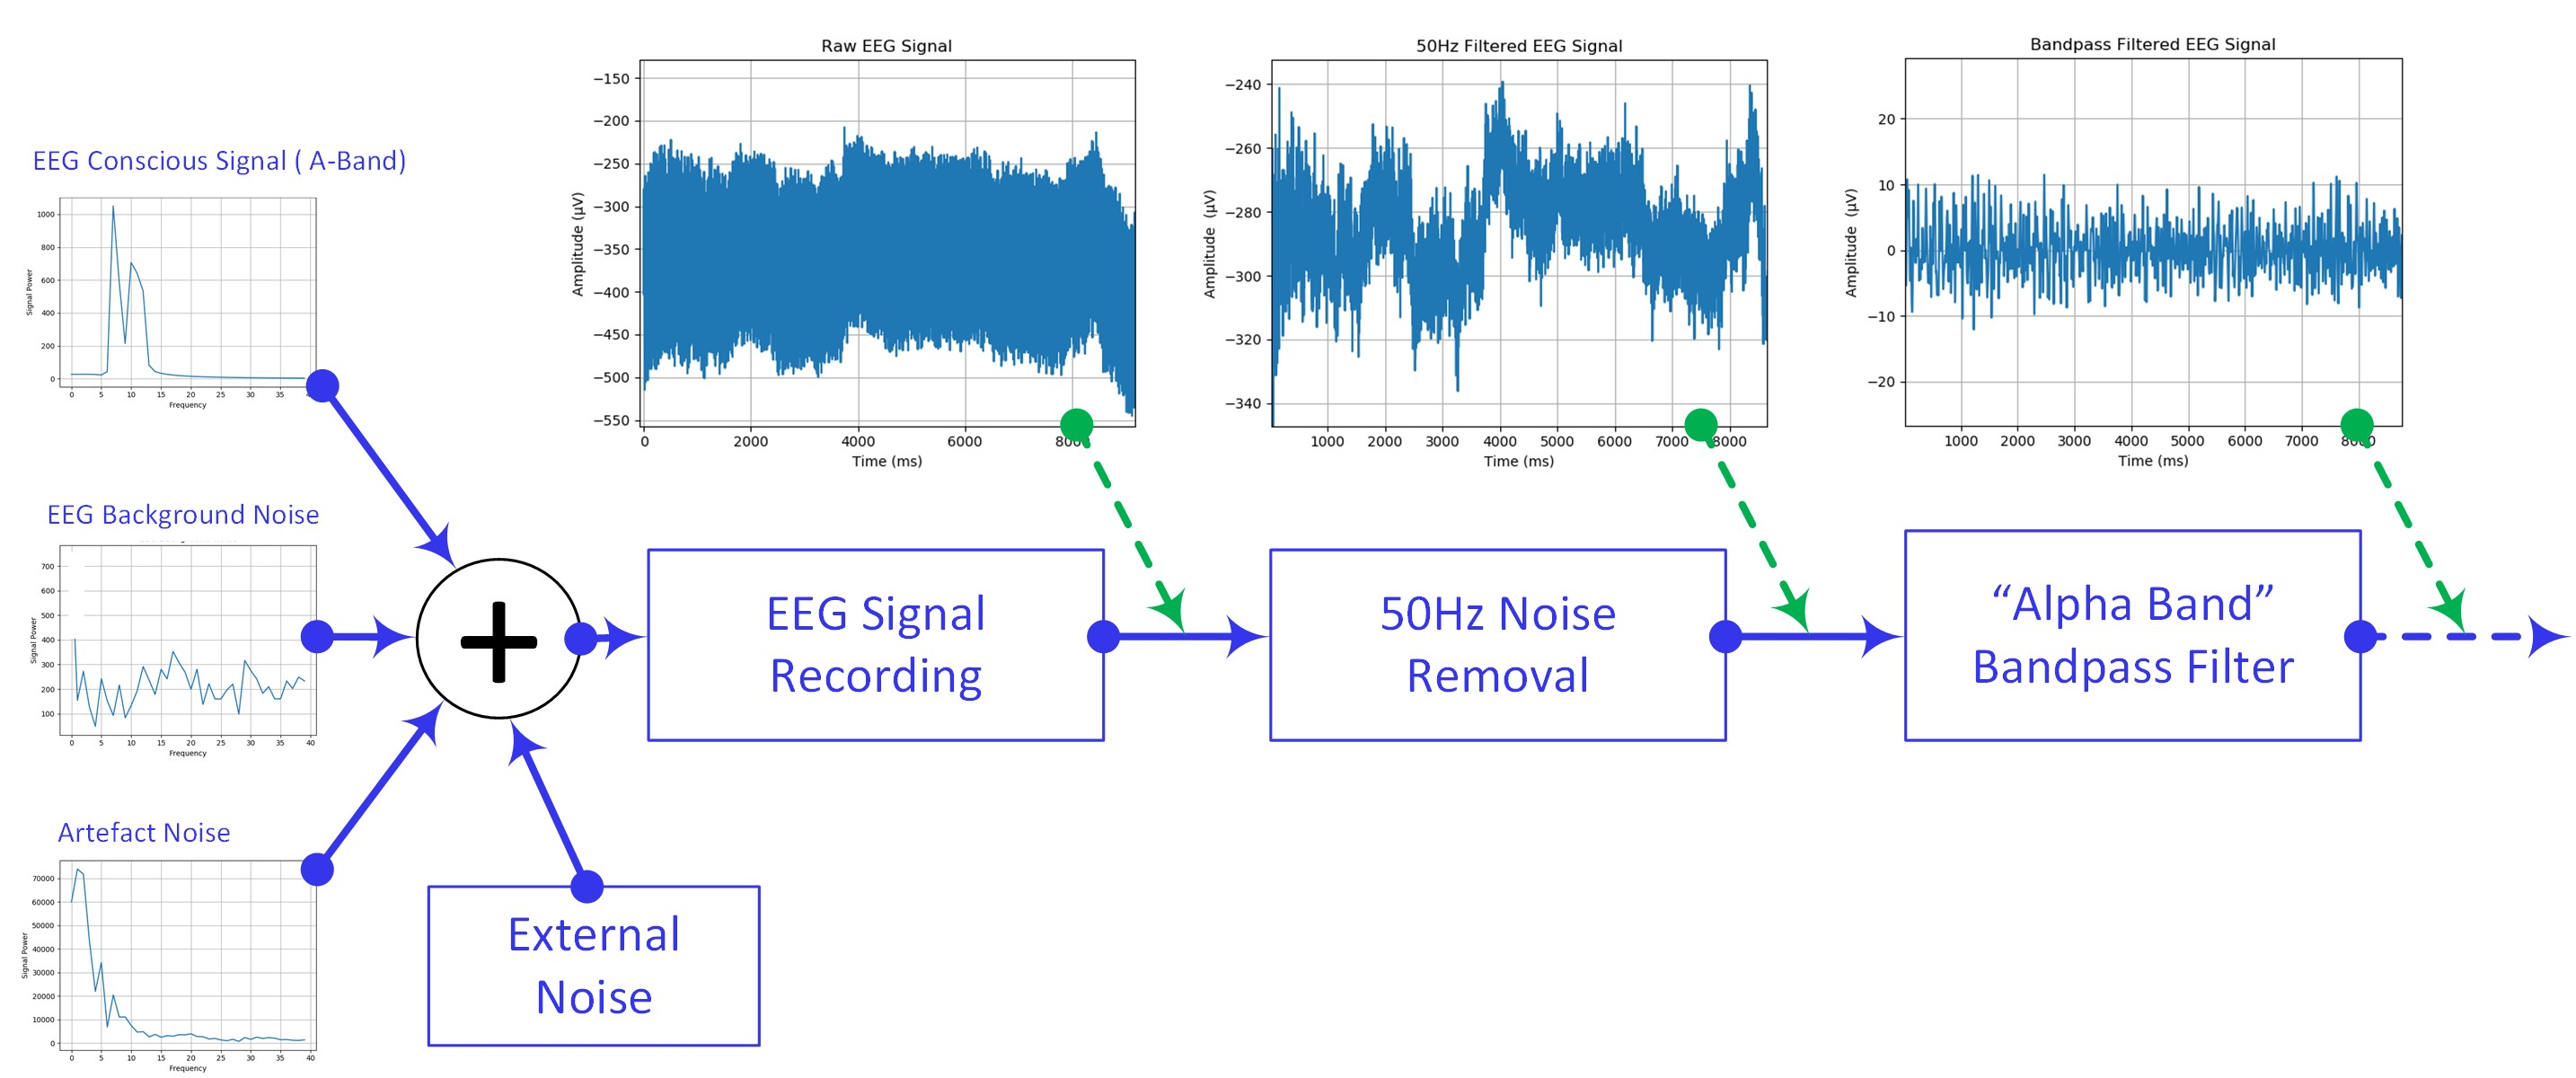
\includegraphics[width=\linewidth]{Figures/EEGsignals.jpg} 
%	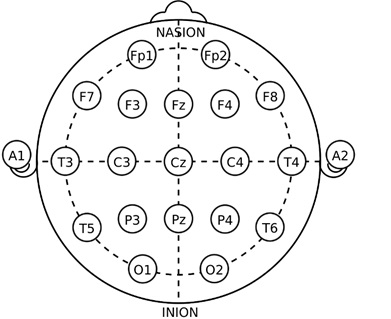
\includegraphics[width=8cm]{Figures/Brain_I20.jpg} 
	\caption{EEG Signals and Preprocessing} 
	\label{EEGsignals} 
\end{figure}





 In the sample domain, a clean EEG recording can be expressed with Equation \ref{eeg_signal}, where M represent the recorded clean EEG signal.In   Equation  \ref{eeg_signal} the components A[n] and B[n] correspond to noise and their sum can be represented with R[n]. 

\begin{equation}
M[n]=A[n]+B[n]+C[n] = R[n]+C[n]
\label{eeg_signal}
\end{equation}


To be able to determine the SNR it is essential to specify which component of the EEG recording is considered to be the noise and which the signal. In \citep{Repovs2010} for the calculation of the SNR, noise was considered to be the EEG component recorded during an artefact, while signal was the consciously generated signal. This is reasonable, since the purpose of the corresponding work was related to the SNR during artefact occurrence. In \citep{Porr2018}, in order to calculate the noise wall, the background noise, EEG signal when the subject is relaxed, was considered to be the minimum noise, while the maximum noise was the mean of all occurrences of artefact noise. The minimum and the maximum noise values were used to calculate the uncertainty (\textrho) of the noise, which in the basis for the calculation of the SNR wall. For the calculation of the SNR, the noise power was considered to be the noise uncertainty multiplied by the minimum noise variance, while the signal power was the consciously generated signal power of paralyzed subject.

The work of this project is different from the work in \citep{Porr2018}  since the aim now is to compute the SNR for EEG signals recorded during motor imagery activities that is, when the subject concentrates on performing a mental activity, and then compare the SNR with the SNR wall to determine if a safe detection can be made.   To this end:
\begin{enumerate} [label=\alph*)]

	\item The subjects are instructed to avoid any body activities that result in artefact noise. 
	\item The subjects are instructed to remain relaxed for a few seconds at the beginning of each experiment. As in \citep{Porr2018} the recorded signal for this time period corresponds to the background noise B[n]. After this time interval, the subject concentrates on carrying out a mental task. The recorded signal for this time interval correspond to the signal component C[n]. Therefore, it is not necessary to use the EEG signals from a paralysed subject.
	\item The calculation of the SNR will be based on the ratio of the variance of the signal component C[n] to the variance of the noise component B[n]. Any artefacts during the EEG recording will contaminate either the noise component, or the signal component, or both, according to the time of occurrence of the artefact. For this study, multiple EEG recordings were obtained. The time plot of these recordings were examined in order to check if the signal contains signal level fluctuations due to artefact. In the case that a non-intentional artefact was identified in a recording, then the EEG recording was discarded. However, there is no quarantine that the rest of the EEG recordings are completely free from artefacts.

\end{enumerate} 

As described in part (b) above, the noise component B[n] and the conscious signal component C[n] will be obtained from different time intervals in the EEG recording. Artefact signals are non-stationary, in the sense that they don’t behave the same way at all times. For example, an artefact might occur due to a non-intentional eye movement during the period of recording the relax signal only. Since the SNR is computed using EEG signals recorded during different time periods, Equation \ref{eeg_signal} can be re-written as shown in Equation  \ref{eeg_signal2}. 


\begin{equation}
M[n]=(B[n]+A_1 [n])+(C[n]+A_2 [n])
\label{eeg_signal2}
\end{equation}

For the purpose of this work, it is assumed that the recorded EEG signals are free from artefacts, therefore the components A1[n] and A2[n] are equal to zero.  Background EEG noise exists in all frequencies of the EEG, while motor imagery brain activities affect only specific frequencies. Therefore, to calculate the SNR it is essential that the EEG signal is bandpass filter in order to isolate the frequency band of interest. The filter signal D[n] is given by Equation \ref{eeg_filter1}, where F[n] is the transfer function of the filter. Equation  \ref{eeg_filter1} can be writen as shown in Equation  \ref{eeg_filter2}, where N[n] is the filtered noise signal and S[n] is the filtered conscious signal. 


\begin{equation}
D[n]=(B[n]+C[n])*F[n]
\label{eeg_filter1}
\end{equation}


\begin{equation}
D[n]=B[n]*F[n]+C[n]*F[n]=N[n]+S[n]
\label{eeg_filter2}
\end{equation}

The SNR can be computed by dividing the variance of the signal with the variance of the noise, as shown in Equation \ref{snr1} and then converted to decibels, if necessary. 


\begin{equation}
SNR = \frac{Signal Power}{Noise Power} = \frac{\sigma_{S}^2 }{\sigma_{N}^2 }
\label{snr1}
\end{equation}

As stated in the Experiment Procedure (Section 3.2), a number of experiments will be conducted where the noise signal is assumed to be the EEG signal obtained when the subject is relaxed. It is expected that for a given subject the noise signal must not change. To ensure a more accurate figure for the noise, the mean of the noise measured between all experiments can be used. Another way to view this is through the noise uncertainty factor (\textrho), a factor that specifies how the noise of a subject is expected to change. Since each subject will carry out a number of experiments, with the background noise recorded at the beginning of the experiment when the subject is relaxing, the maximum and the minimum noise variances between the different experiments can be used to compute the noise uncertainty, according to Equation \ref{rho}.

\begin{equation}
Noise  Uncertainty:  \rho = \sqrt{\frac{\sigma_{Rmax}^2 }{\sigma_{Rmin}^2 }}
\label{rho}
\end{equation}

Where:  $\textsigma_{Rmax}^2$ is the maximum noise variance between the different experiments. 

\hspace{12mm} $\textsigma_{Rmin}^2$ is the minimum noise variance between the different experiments.
 
The noise variance based on the noise uncertainty can be computed using  Equation \ref{noiseV},  while the SNR can now be computed using  Equation \ref{snr2}.

\begin{equation}
Noise  Variance: \sigma_{R,n}^2 = \rho * \sigma_{Rmin}^2 
\label{noiseV}
\end{equation}

\begin{equation}
SNR =  \frac{\sigma_{C}^2 }{\sigma_{R,n}^2 }
\label{snr2}
\end{equation}


\subsection{\bf{Data Analysis Method:}}
This section describes the steps needed in order to determine the SNR wall for each subject, calculate the SNR for each experiment and determine if it is possible to detect the EEG signal. The steps needed are the following:
\begin{description}
 	\item[Step1: ] Filter the EEG signal to remove any external noise such as the 50Hz mains noise.
	\item[Step2: ] Band-pass filter the EEG recording to remove all frequencies except the alpha band frequencies (8Hz to 12Hz). 
	\item[Step3: ] 	For each subject isolate the first part of the recording of each experiment that corresponds to the relaxing period. Calculate the noise variance for each experiment. Find the maximum and the minimum noise variances. ($\textsigma_{Rmax}^2$) and ($\textsigma_{Rmin}^2$).
	\item[Step4: ] For each subject use Equation \ref{rho} to calculate the noise uncertainty (\textrho). Use Equation \ref{noiseV} to calculate the noise variance ($\textsigma_{R,n}^2$) for each subject. 
	\item[Step5: ] For each subject and each experiment calculate the conscious signal variance  $\textsigma_{C}^2$ for the samples corresponding to the first second of the conscious activity of the subject. Use Equation \ref{snr2} to determine the SNR. Repeat for the next segment of the EEG signal. The distance between adjacent segments is 500ms. 
	\item[Step6: ] For each subject and each experiment compare the SNR wall from  \citep{Porr2018} and the SNR from step 5 to determine if a safe detection can be made.  
  
\end{description}



\newpage
\section{\centerline{Results and Discussion}}
\label{sec:results}


\vspace {15pt}
The results presented in this section are based on the EEG recordings of the author of this report. For more conclusive and reliable results, it is usually required to perform experiments with a number of subjects. The initial intention, described in the experimental methodology, was to get recordings from a number of willing participants. This requires the prior authorization of the Ethics Committee of the University.  To this end, an application has been submitted to the Ethics Committee. This authorization has not been granted yet. 

The EEG recording presented, were recorded during the week 12 to 18 of August 2019. The experiments were conducted in the Laboratory (Building: Rankine Room: 509), using the experimental setting described in the “Methodology” section. The EEG recordings were obtained using the “Comedirecord” (Porr B. , ComediRecord) open source oscilloscope software for Comedi. Through this software, the EEG signal samples were filtered and displayed as a time domain signal, as well as a frequency spectrum, zoomed in the range of the alpha band frequencies. Displaying the frequency spectrum of the EEG signal, is essential, since this provides feedback to the subject. The EEG recordings were saved in the “csv” format so that they can be directly processed.
 
The EEG signals received from the EEG electrodes were first amplified by an amplifier with a gain of 50. The gain of the amplifier was initially set to 500. During the initial tastings it was found that in some recordings, during artefacts, the 50Hz mains noise combined with the artefact signal was too high, causing the analogue-to-digital converter (ADC) to clip the signal. Thus the sampled values were close to a square waveform, creating frequency harmonics. To avoid this, the gain of the amplifier was reduced to 50. The EEG signals were then sampled by the data acquisition with a 1000Hz sampling frequency, using a 24-bit sigma/delta ADC. The maximum input voltage of the ADC is ±1.33V, resulting in a signal resolution of 0.158  \textmu V/LSB. The amplitude of the EEG signals is in the order of a few  \textmu V to few tens of  \textmu V. Much higher amplitudes are observed during artefacts. Considering that the gain of the amplifier is 50, it can be calculated that a low EEG signal of say 1 \textmu V can be sampled with 316 sample levels. Expressed in another way, a 1 \textmu V EEG signal will be amplified to a 50  \textmu V signal by the amplifier and then converted to a binary code equal to 316 by the ADC.
   
The processing of the recorded data was done with two programs developed in Python. The first one, “EEG Plot.py” was used to produce the required waveforms and graphs, while the second, “EEG SNR.py” was used to perform the necessary calculations, in order to determine the SNR or the recorded EEG signals. Both programs use an open source IIR filter class obtained from GitHub (https://github.com/poganyg/IIR-filter/blob/master/src/IIR2Filter.py). The software used, as well as the EEG recording files are available on GitHub (https://github.com/nikolaskyr/EEG-Signals-SNR-Calculation).
 
Following the experimental methodology, defined in the “Methodology” chapter, a number of experiments were conducted, where the subject was concentrating on mentally performing two tasks. In the first task, the subject was trying to consciously move the window displaying the real time recorded spectrum on the screen of the computer. Throughout this effort, the subject was also observing the actual spectrum on the screen, as a means of feedback, and consciously trying to increment the 10Hz peak. The window displaying the EEG spectrum was placed in the centre of the screen, while the subject was trying to move it to the left, right, up and down. In the second task, the subject was looking at his real time EEG spectrum, and consciously trying to increase the peak at the 10Hz, 20Hz and 30Hz. The experiments conducted are listed in Table \ref{tasks} below:

\begin{table}[hbt!]
	\caption{Experiment Tasks}
	\label{tasks}
	\centering
	\begin{tabular}{|c|c|l|}
	\hline
		Task & File Name & Function \\
		 \hline\hline
		1 & Task1 & Try to consciously move the spectrum window to the left \\
		2 & Task2 & Try to consciously move the spectrum window to the right \\
		3 & Task3 & Try to consciously move the spectrum window up  \\
		4 & Task4 & Try to consciously move the spectrum window down \\
		5 & Task5 & Try to consciously increase the 10Hz peak on the spectrum \\
		6 & Task6 & Try to consciously increase the 20Hz peak on the spectrum \\
		7 & Task7 & Try to consciously increase the 30Hz peak on the spectrum \\
		 \hline
	\end{tabular}
\end{table}

At the beginning of each experiment, the subject was relaxed for two-three seconds before trying to perform the task. The EEG recording obtained during this time is used as a reference for the noise calculation.  After this relax period the subject was concentrating on the specific task of the experiment. Before conducting the actual experiments, a number of non-recorded attempts were made as a form of familiarisation of the system and training of the subject.

The presentation and analysis of the results of this work are presented in two sections.  The first section investigates the effect of the conscious task on the 10Hz peak. The second section investigates the effect of the conscious task on the SNR ratio. For both investigations, the recorded signals were first filtered with a 10th order Chebyshev notch filter to remove the 50Hz mains noise. The cleaned EEG recordings were the filtered with a 10th order Chebyshev bandpass filter to isolate the alpha band frequencies (8Hz to 12Hz). The 50Hz band-stop filtered EEG signal as well as the spectrum of the unfiltered EEG recording for Task 1 are shown in Figure \ref{eegraw}a and Figure \ref{eegraw}b respectively. From the time domain signal it can be seen that even though the subject was supposed to avoid anything that could lead to an artefact, in some cases there are some minor fluctuations in the signal that correspond to artefacts. From the spectrum of the signal it can be seen that the unfiltered signal contains noise at 50Hz, as well as a high DC offset.    

\begin{figure}[hbt!]
	\centering
	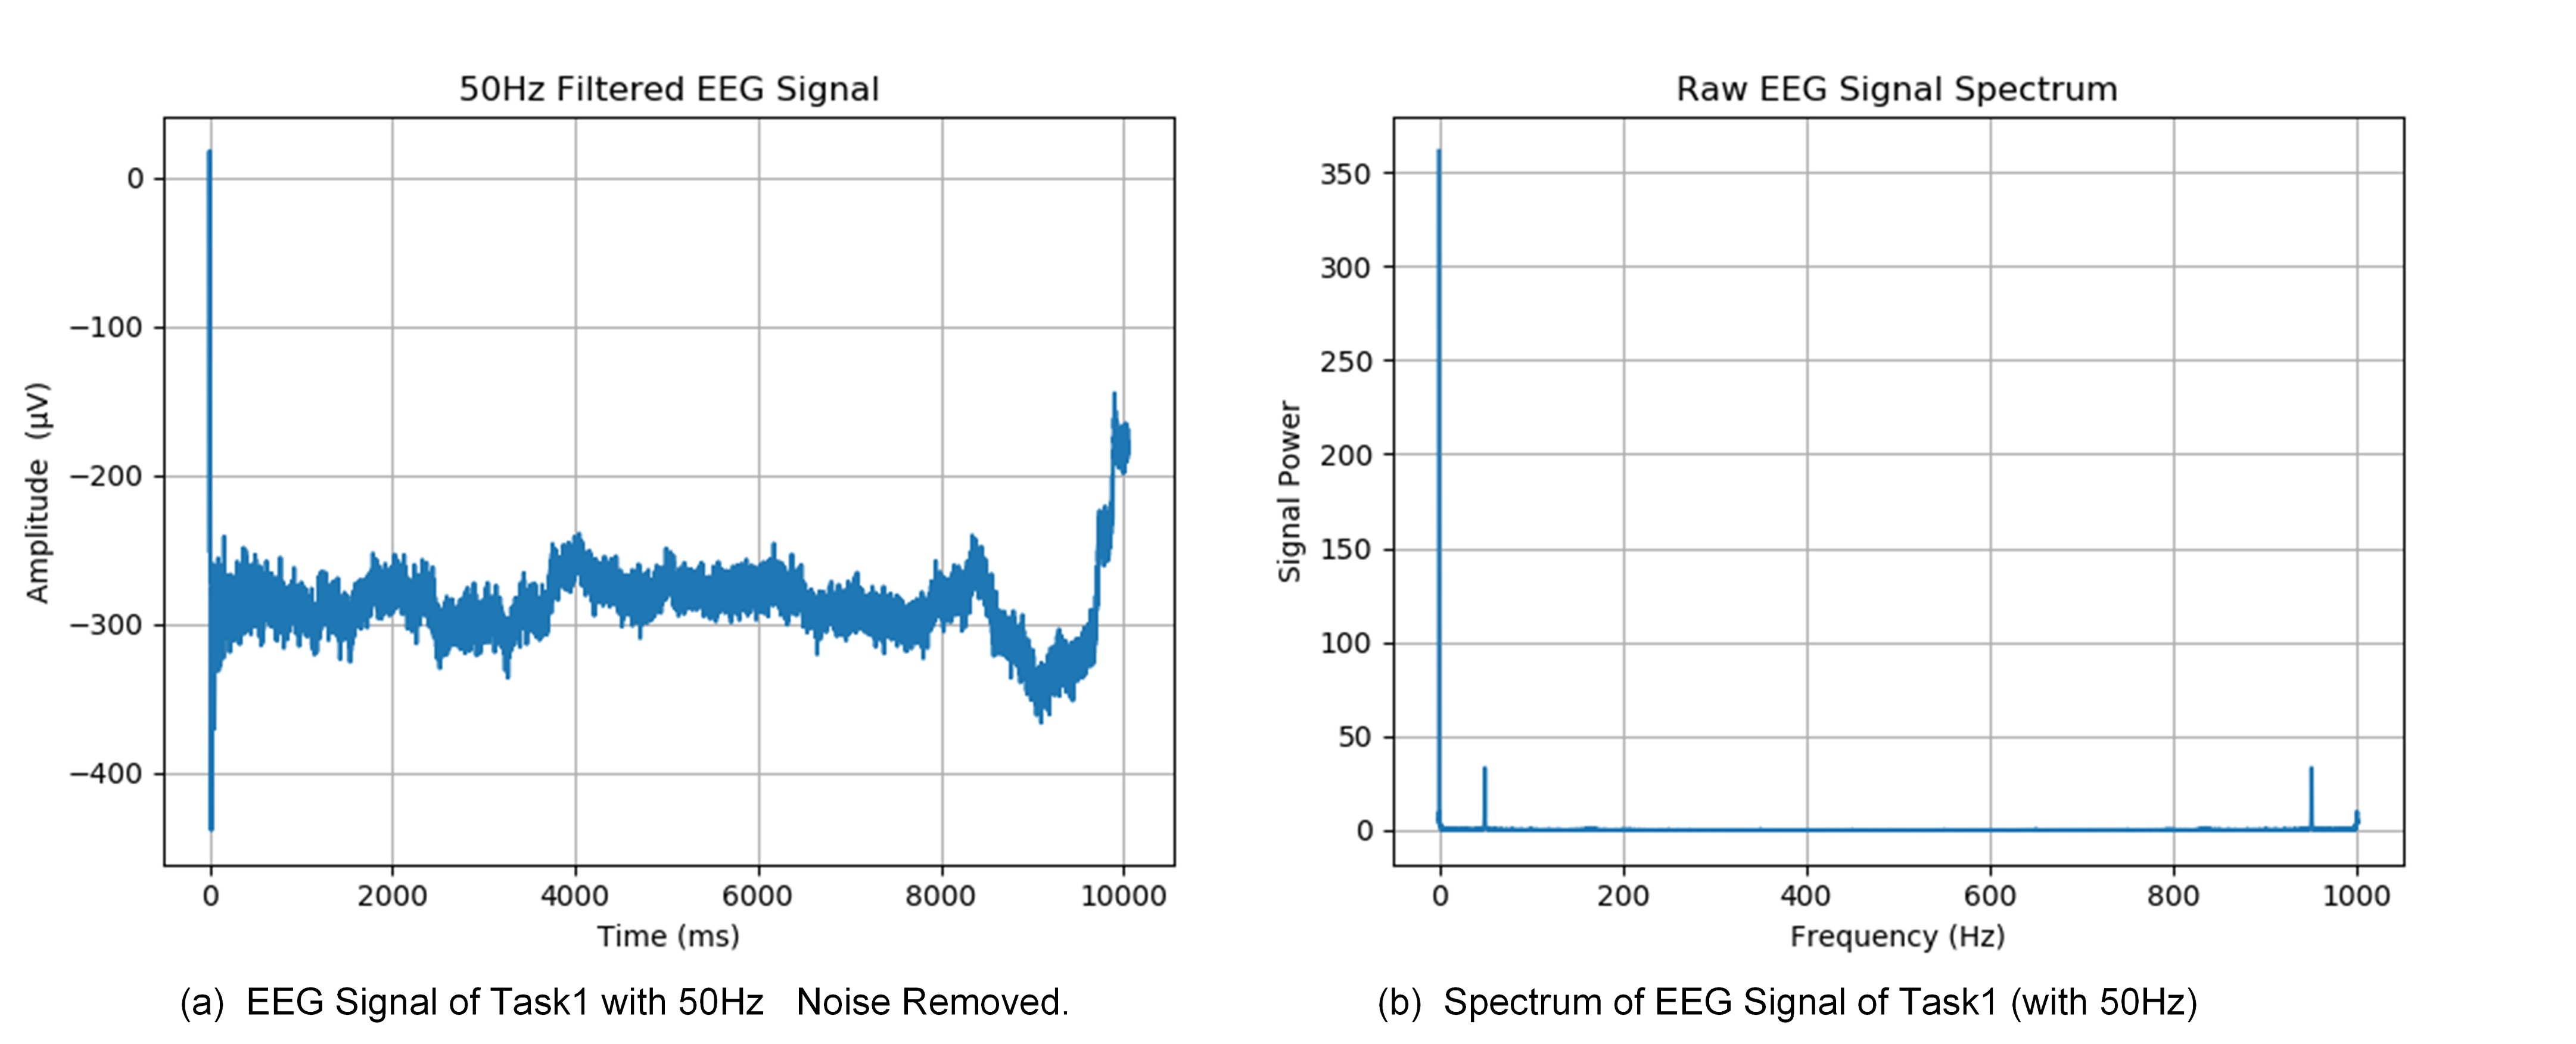
\includegraphics[width=\linewidth]{Figures/eeg_raw.jpg} 
%	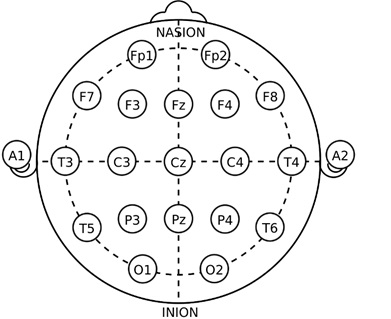
\includegraphics[width=8cm]{Figures/Brain_I20.jpg} 
	\caption{Time Domain and Spectrum of the EGG Signal for Task 1.} 
	\label{eegraw} 
\end{figure}

 
The investigation of the EEG signal was done using overlapped one second EEG signal segments. To account for the possible delays of the filters and the time required by the subject to relax, the relax sample segments were taken from the samples corresponding to 1.5 seconds after the EEG recording was initiated. The conscious signal segments were taken from four seconds up to eight seconds since the start of the recording. The analysis of the conscious signal was done on one-second overlapped segments as shown in Figure \ref{segments}.

\begin{figure}[hbt!]
	\centering
	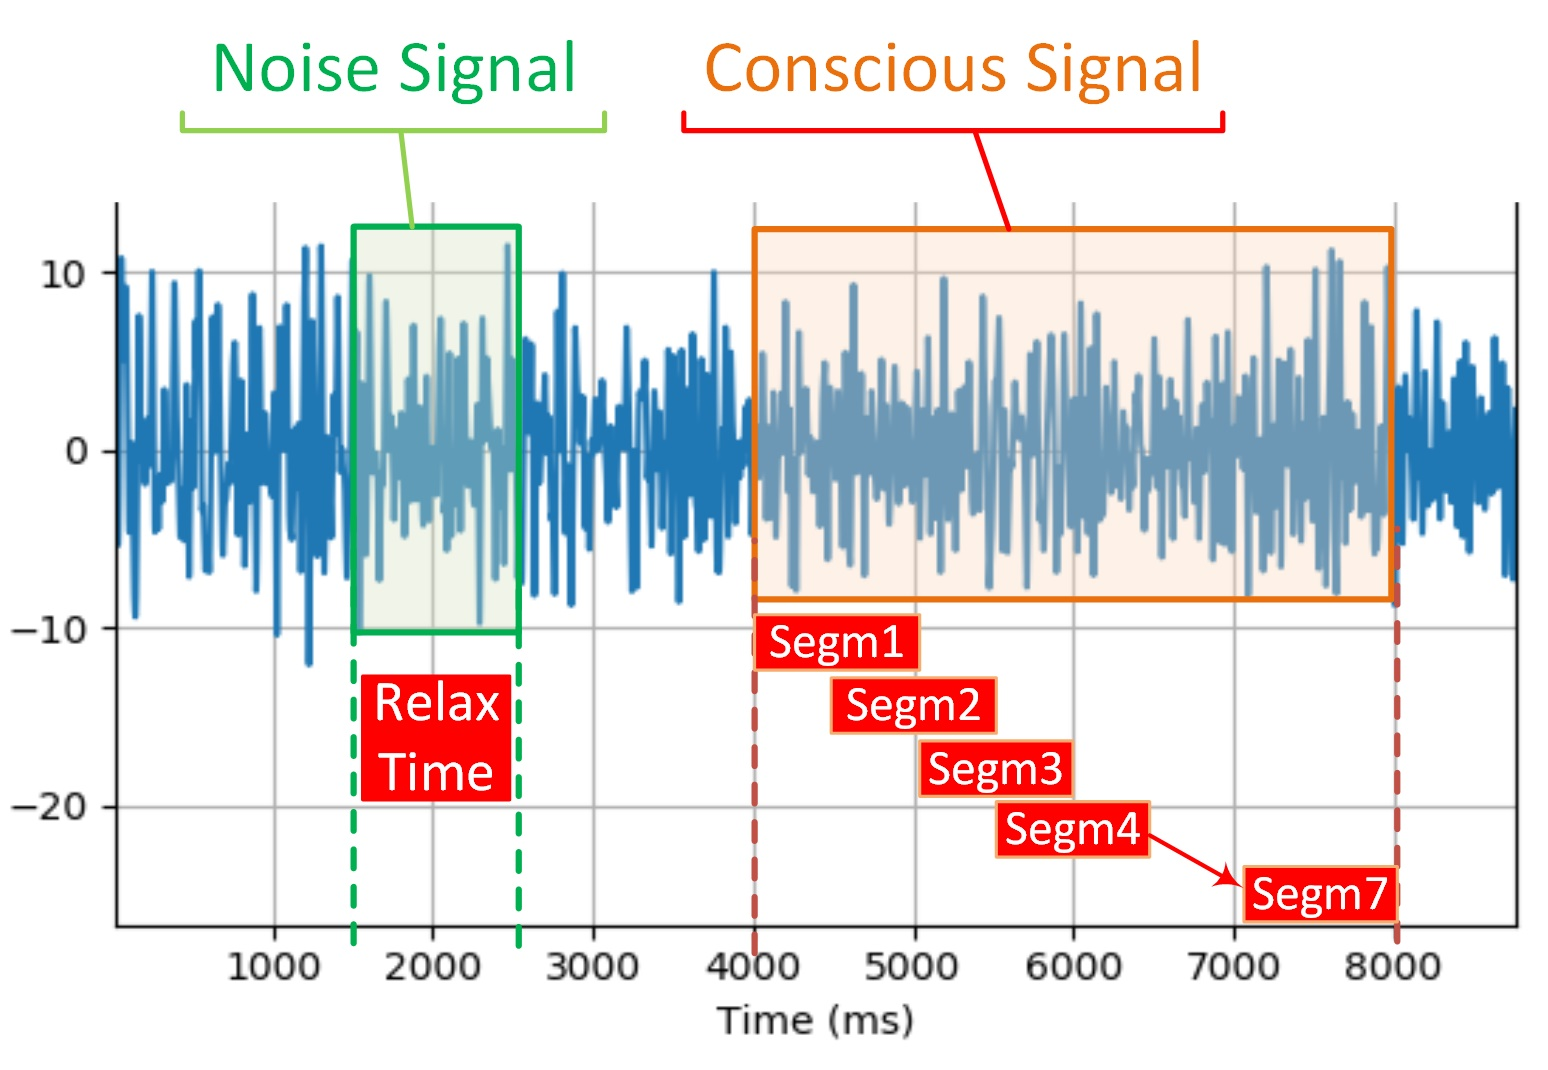
\includegraphics[width=\linewidth]{Figures/segments.jpg} 
%	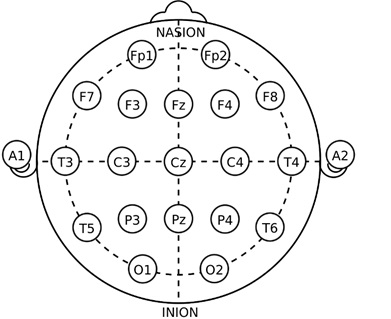
\includegraphics[width=8cm]{Figures/Brain_I20.jpg} 
	\caption{Segmentation of the EEG Signal.} 
	\label{segments} 
\end{figure}

\subsection{\bf{The 10Hz Peak Investigation:}}
The motor imagery brain activity has an effect on different frequencies in the alpha and the beta bands \citep{Pfurtscheller2000, Khulman1978}. One of the investigations of this project is related to the effect of the conscious brain activity on the 10Hz frequency. To this end the spectrum of the alpha band EEG signal obtained during the relax period is examined with respect to the spectrum of alpha band EEG signal obtained during the conscious brain activity period. Figure \ref{relaxed} shows the alpha band spectrum of the recorded signal during the relaxed period. Because imagery move activities affect other frequencies as well, the right part of Figure \ref{relaxed} also shows the frequencies up to 40Hz. 


 \begin{figure}[hbt!]
	\centering
	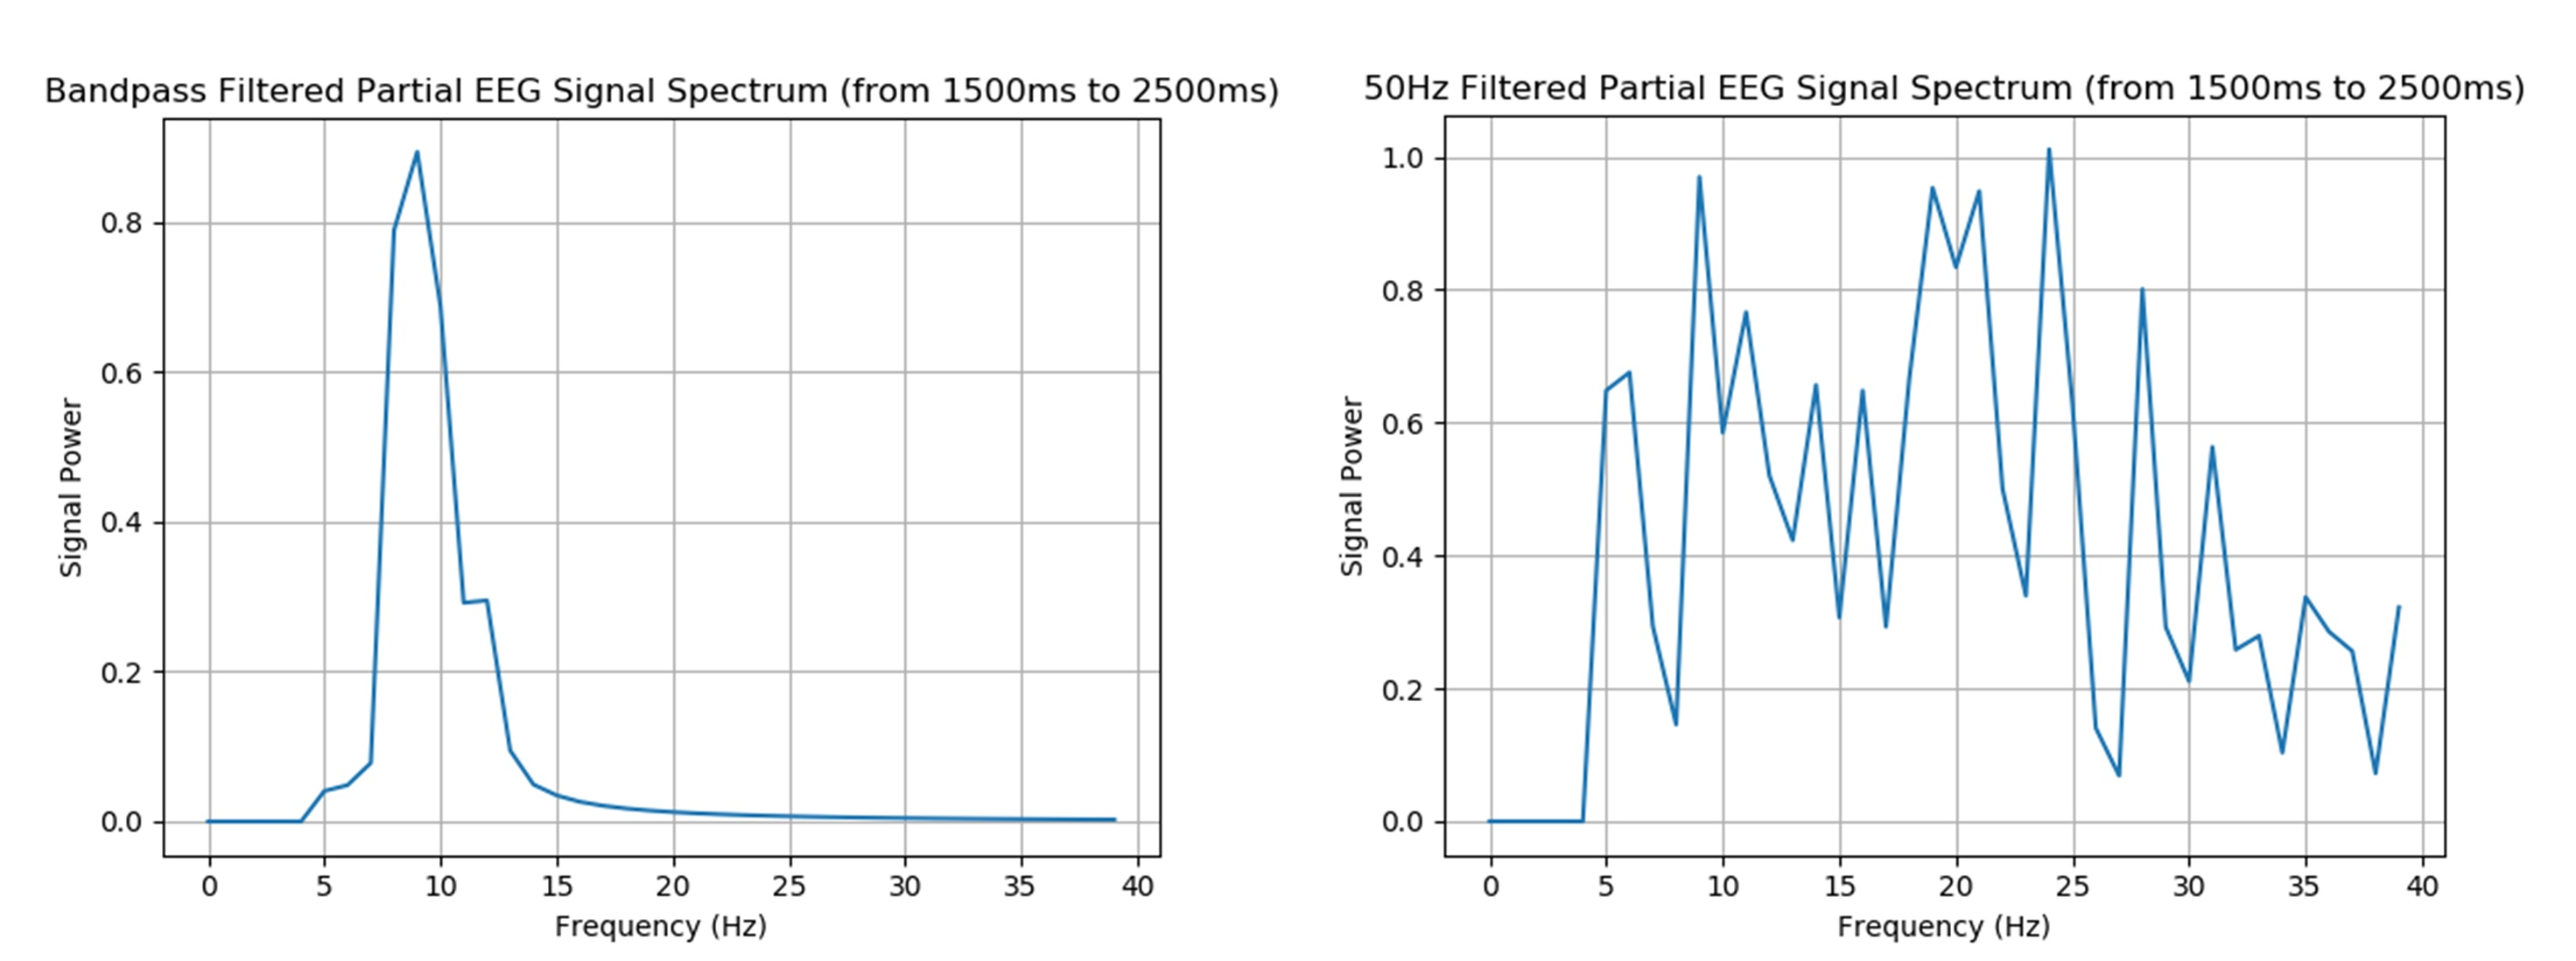
\includegraphics[width=\linewidth]{Figures/relaxed.jpg} 
%	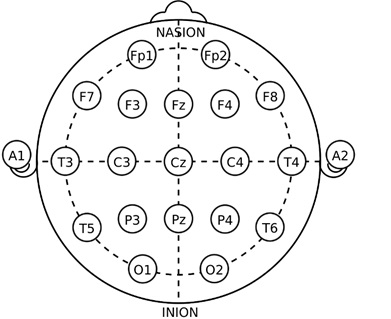
\includegraphics[width=8cm]{Figures/Brain_I20.jpg} 
	\caption{Spectrum of Subject Relax Interval (Task1).} 
	\label{relaxed} 
\end{figure}

From the filtered signal it can be seen that there is a peak at 9Hz, while from the unfiltered signal it can be seen that there are also peaks on other frequencies around 20Hz and 25 Hz. During the relaxed period, for this task, these peaks have a strength close to the strength of the 8Hz or 9Hz frequencies. The waveforms shown in Figure \ref{spectrum1} represent the spectrum during the motor imagery activity, from 4 seconds to 8 seconds. By observing the waveforms it can be seen that there are peaks at all frequencies in the alpha band. By observing the 10Hz peak in Figure  \ref{spectrum1}  are shifted to lower or higher frequencies, therefore the peaks in Figure  \ref{spectrum1}b are due to the peaks occurring at different time intervals within the four second interval. Furthermore, from the waveform of the unfiltered signal, it can be seen that the alpha band peaks are higher than those in the 18Hz to 30Hz zone.



 \begin{figure}%[hbt!]
	\centering
	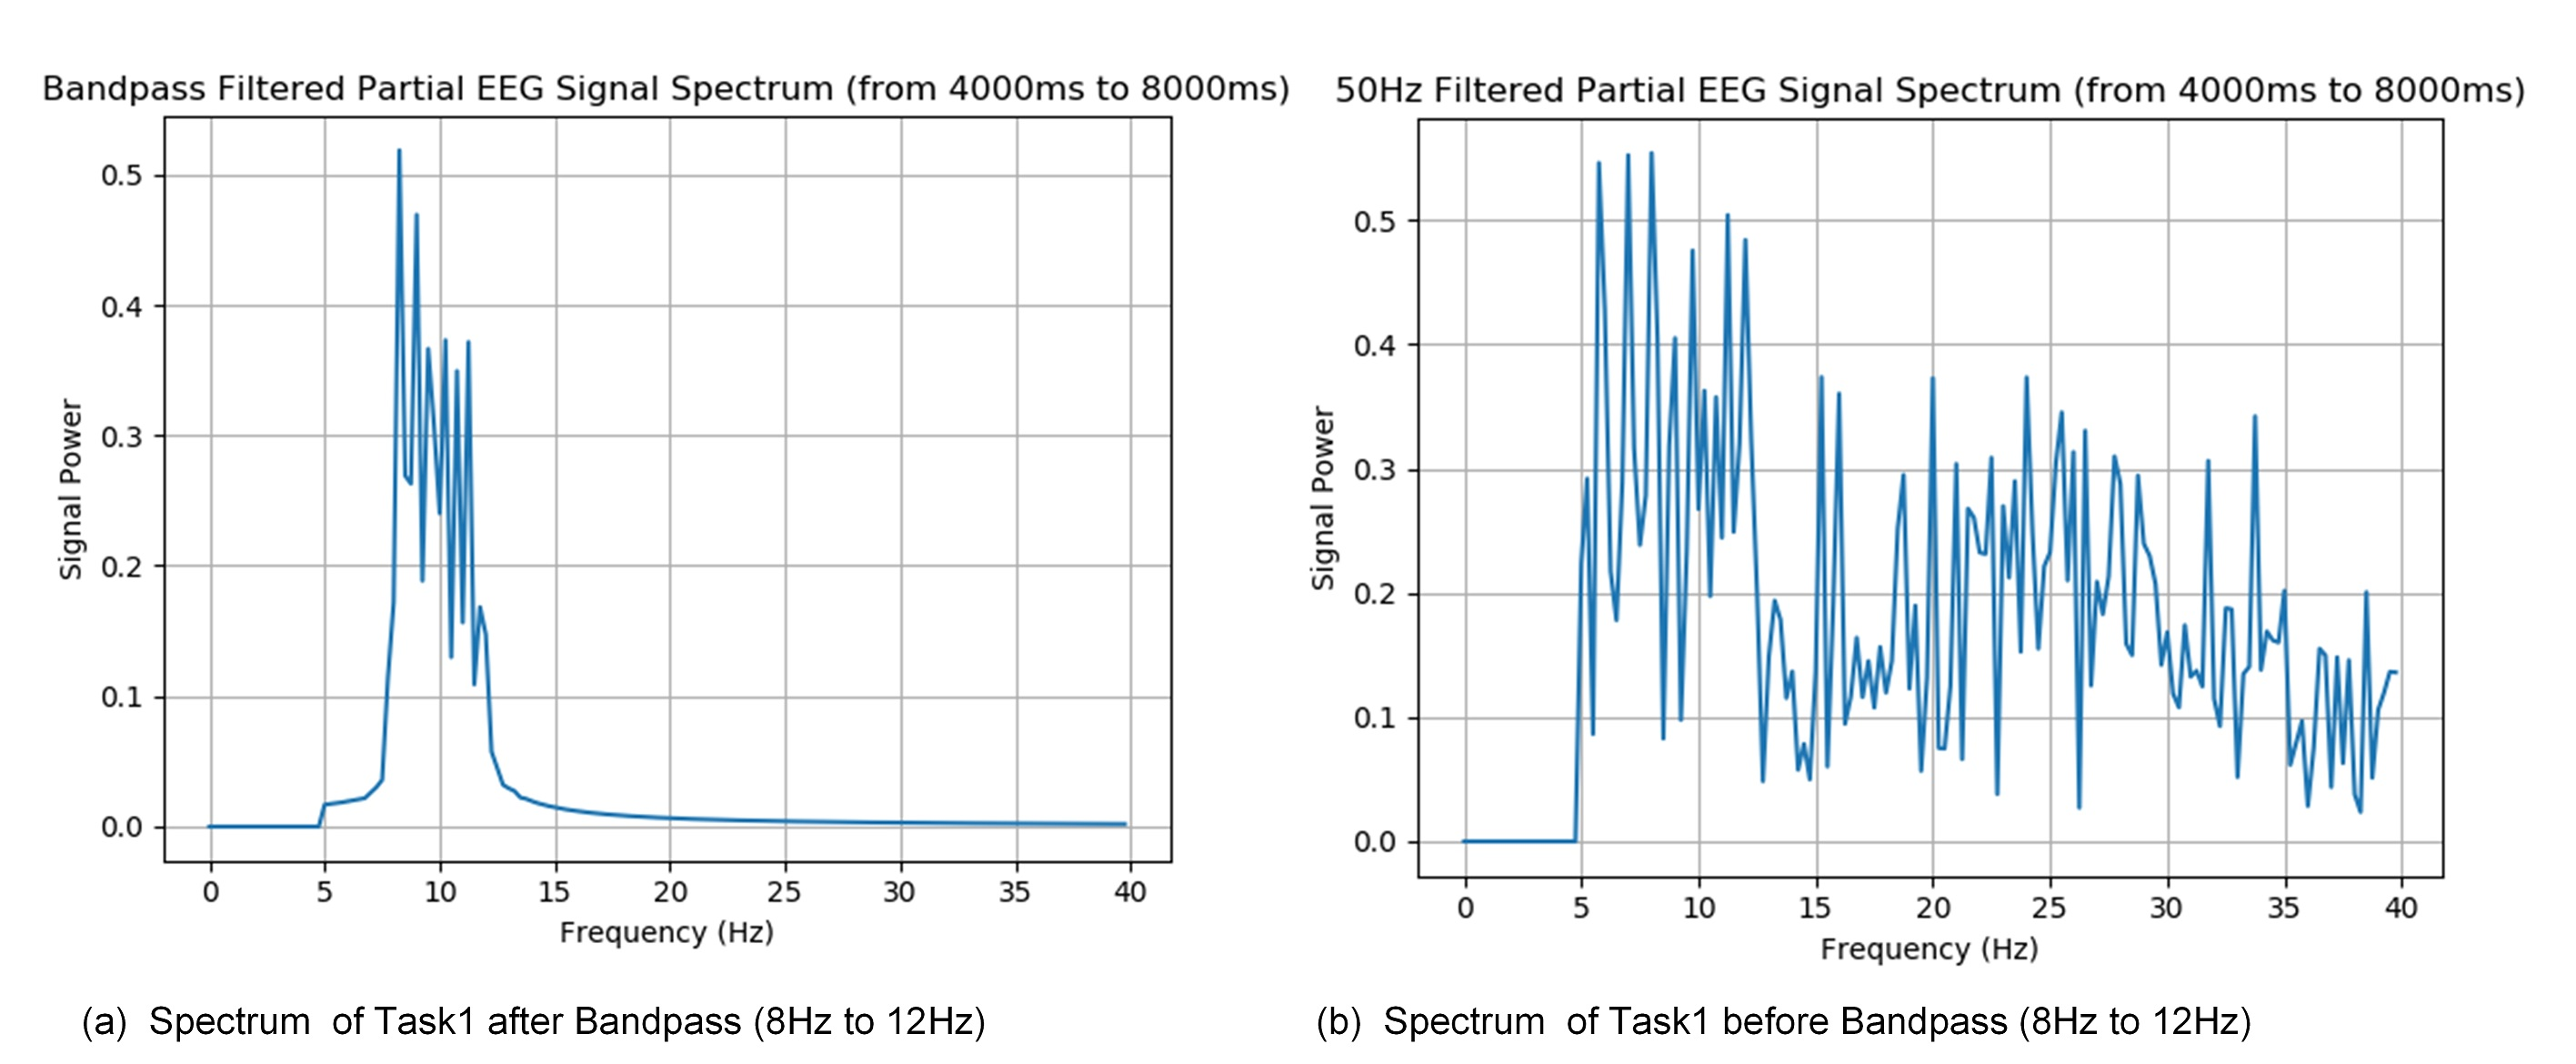
\includegraphics[width=\linewidth]{Figures/spectrum1.jpg} 
%	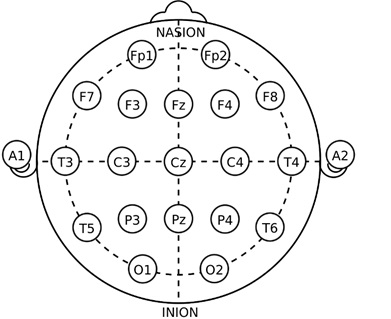
\includegraphics[width=8cm]{Figures/Brain_I20.jpg} 
	\caption{Spectrum for Task1 for the duration from 4s to 8s.} 
	\label{spectrum1} 
\end{figure}



The peaks on each one of the frequencies of the alpha zone shown in Figure \ref{spectrum1}, as well as the spectrum obtained during shorter signal segments were also examined. Figure \ref{task1_10} shows the spectrum for one-second signal segments starting at 4s, 5s, 6s, and 7s. From these spectrum diagrams it can be seen that there is also one distinguished peak around 10Hz, but this shifts either to slightly lower or higher frequencies (9Hz or 11Hz). These peak shifts are in accordance with the observations of \citep{Pfurtscheller2000, Khulman1978}.  


Similar observations can be made by examining the spectrum of the EEG signals in the alpha zone achieved with the rest of the tasks (experiments).  Figure 11 shows the spectrum for the relaxed as well the spectrum for two of the signal segments for each of the tasks 2 to 6. In all cases there always a sharp pick at around 10Hz, while in some cases a second peak is observed. Furthermore, in all experiments there is always a slight shift of the 10Hz peak either towards the 9Hz of the 11Hz frequencies. This characteristic must be taken into consideration in a BCI system looking for a signal change on the 10Hz frequency in order to make a decision on the user’s intent.

\begin{figure}%[hbt!]
	\centering
	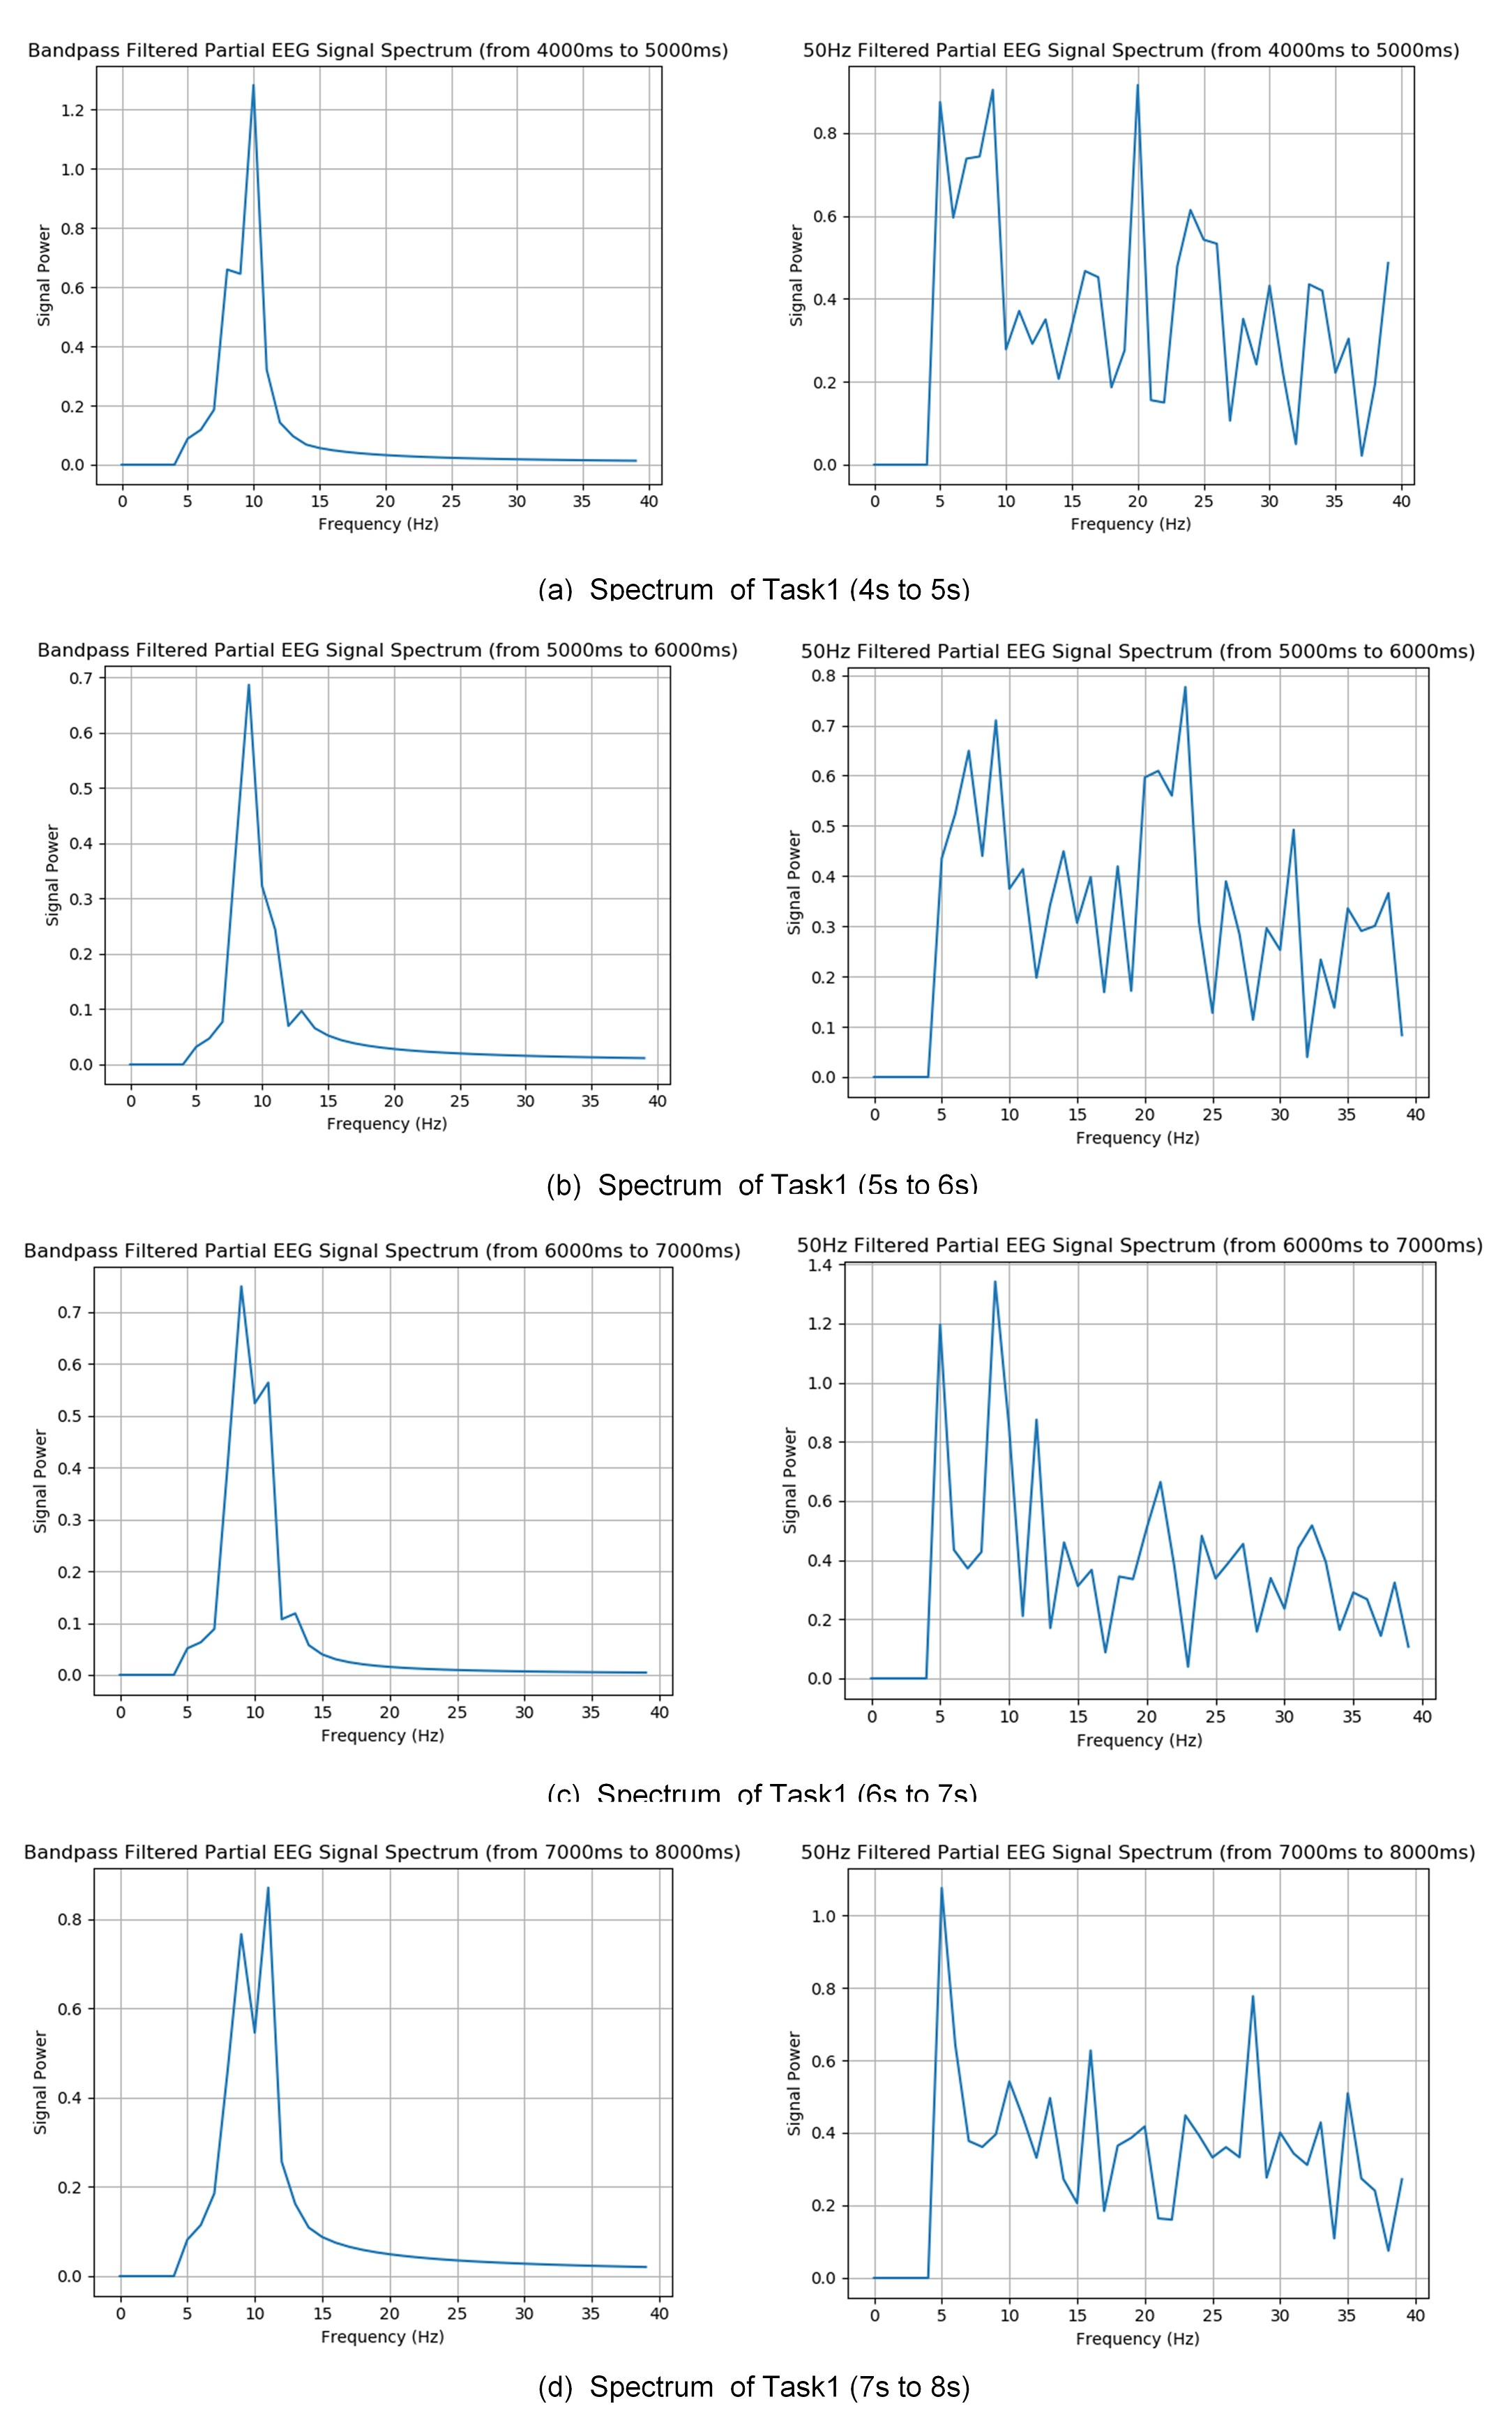
\includegraphics[width=\linewidth]{Figures/task1_10Hz.jpg} 
%	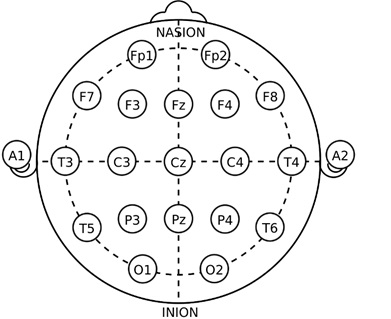
\includegraphics[width=8cm]{Figures/Brain_I20.jpg} 
	\caption{Spectrum for Task 1 (Segments of 1000ms each).} 
	\label{task1_10} 
\end{figure}


During the EEG recordings it was observed that in order to be able to use feedback, by observing the 10Hz peak, it was difficult to achieve. Even though in most cases the 10Hz band was increasing, this was not done by a significand amount. It needs practice and concentration to be able to try to perform a motor imagery operation and at the same time try to control the 10Hz frequency. It is also possible that the effect of the specific imagery move task is eventually a desynchronization event that might reduce the 10Hz instead of increasing it.  A similar case was observed when the motor imagery intent was to try and increase the 10Hz, or the 20Hz or the 30Hz frequency peaks (Figure 12). Some success was though observed when the task was to try to increase the 20Hz peak, however this is most probably the effect of the motor imagery task on the 20Hz frequency, since this is also observed in other experiments. 


\begin{figure}%[hbt!]
	\centering
	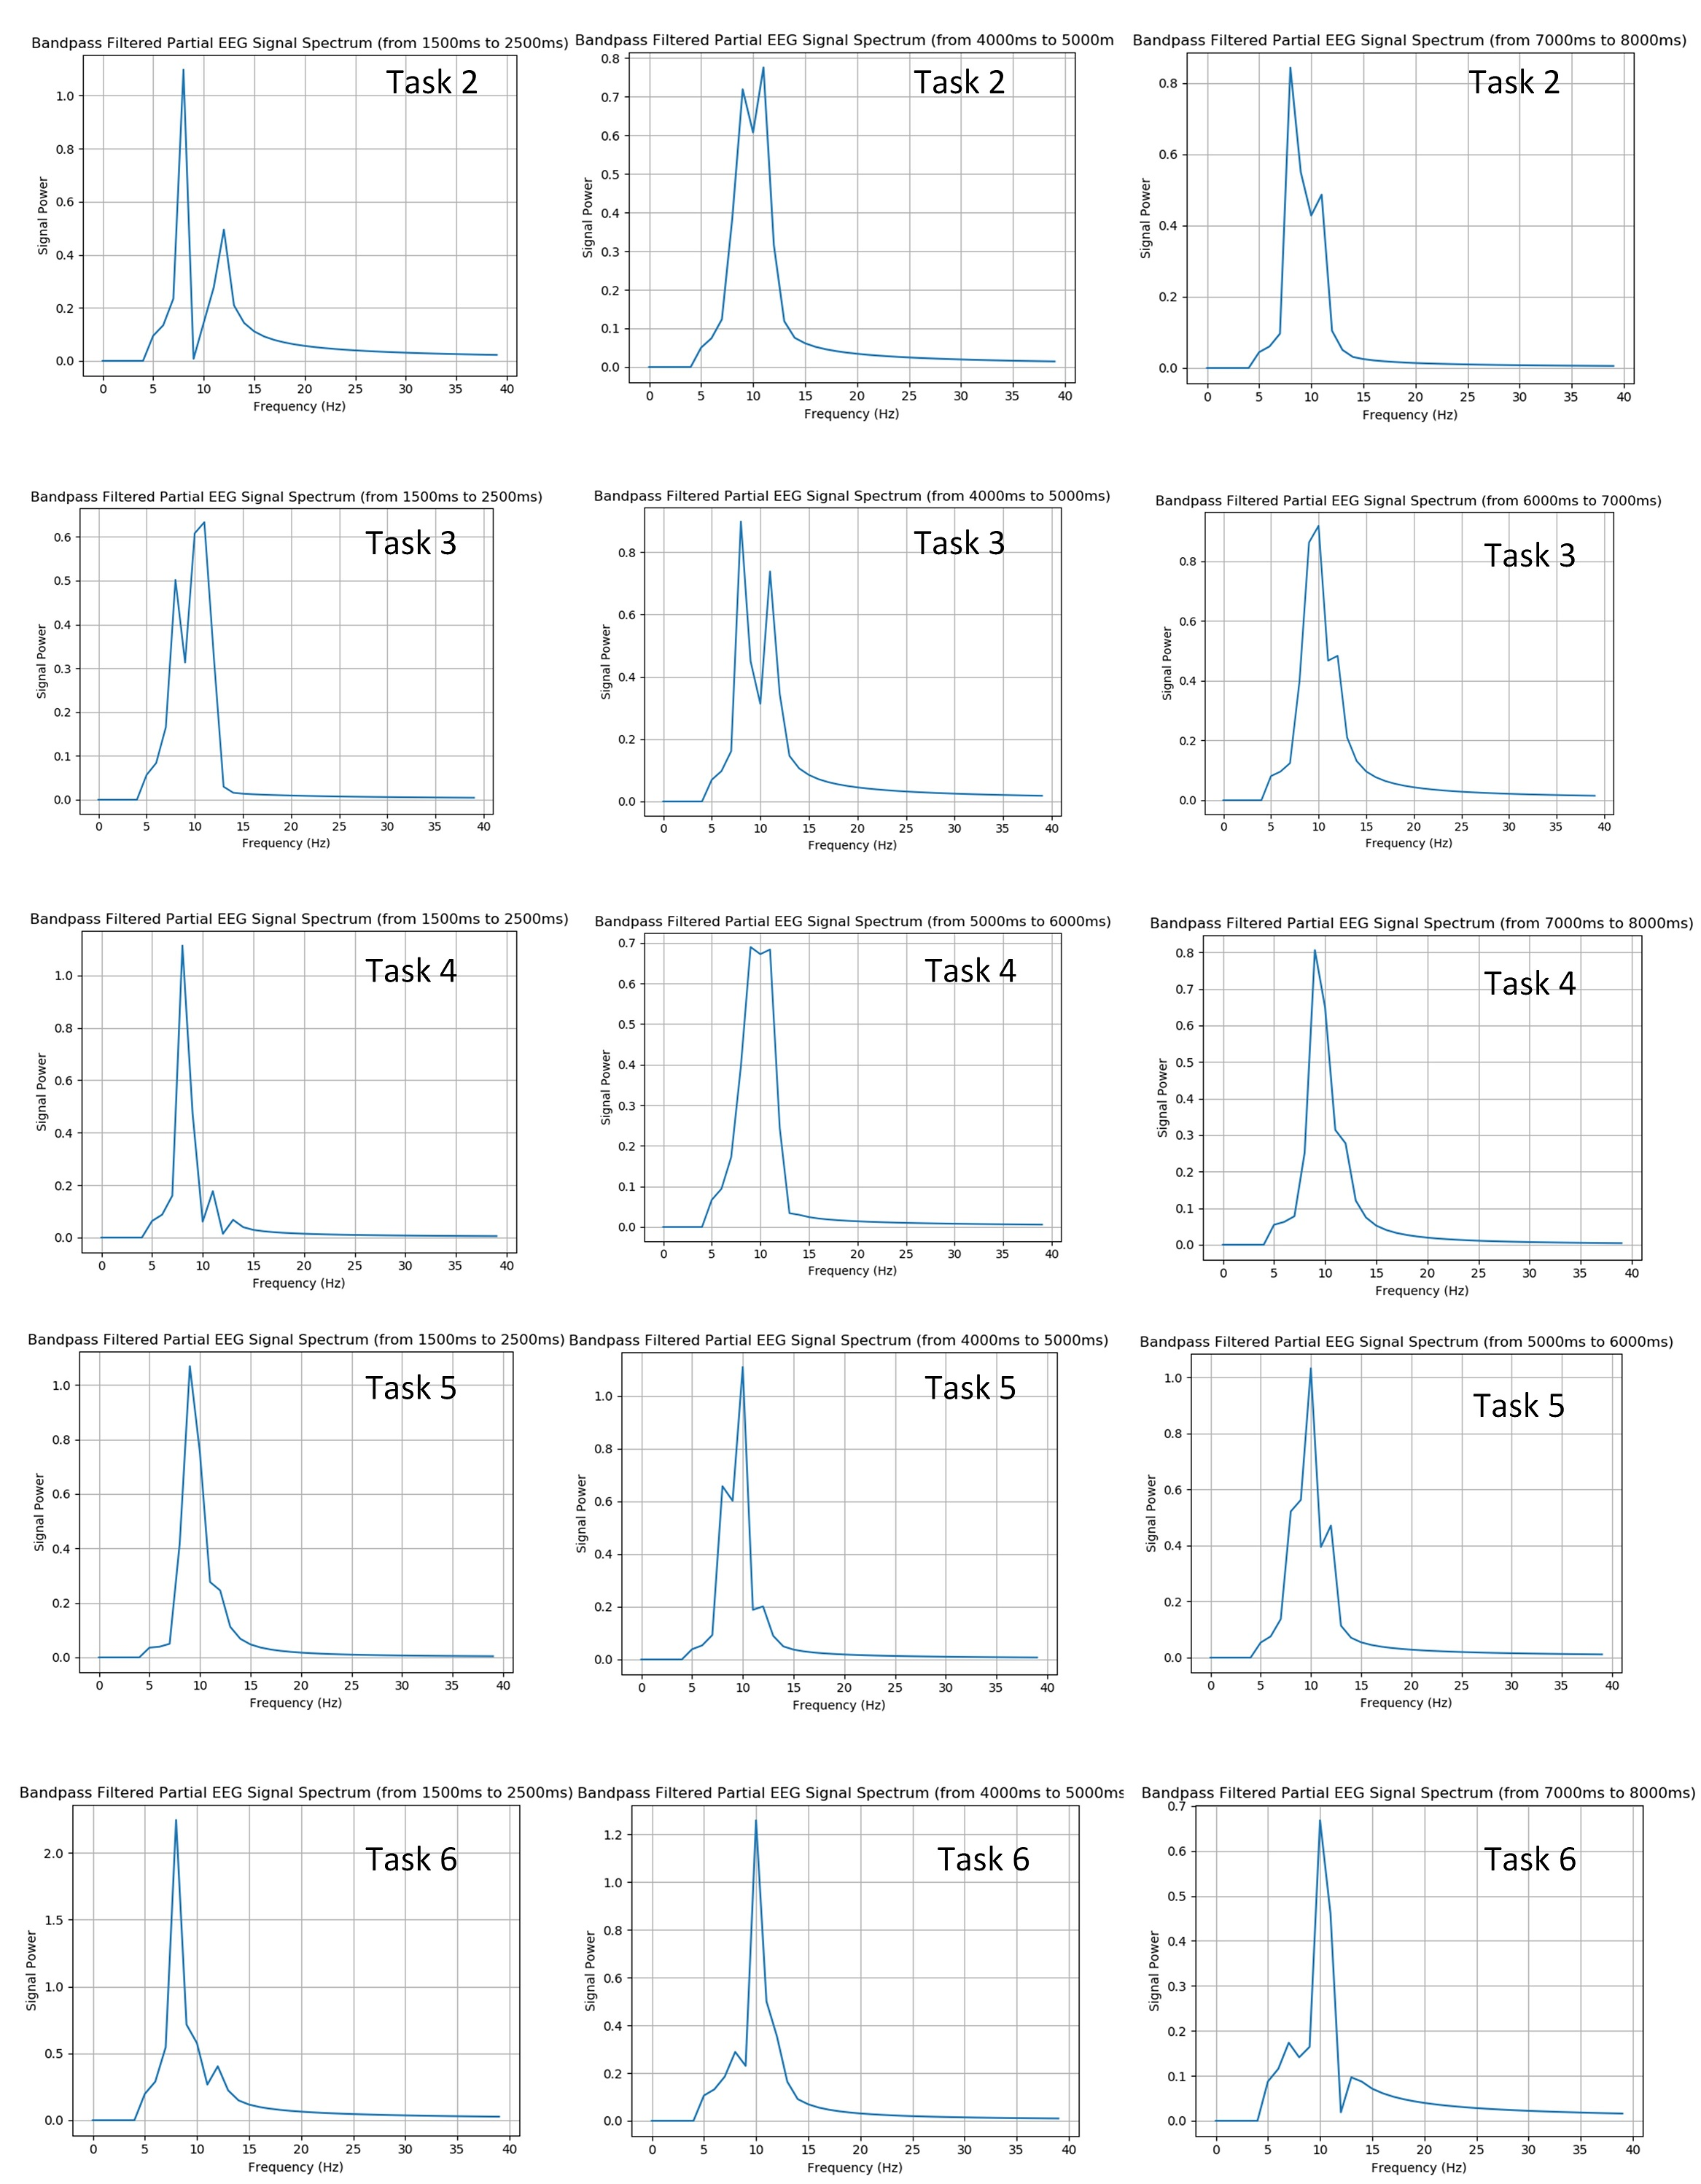
\includegraphics[width=\linewidth]{Figures/filteredAll.jpg} 
%	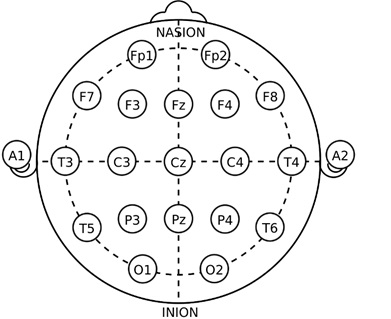
\includegraphics[width=8cm]{Figures/Brain_I20.jpg} 
	\caption{Filtered Spectrum for Task2 to Task6.} 
	\label{all_tasks_filt} 
\end{figure}

By observing the spectrum of the unfiltered signal, it can be seen that the picks in the beta frequency zone are also affected by the motor imagery process. Fluctuations are observed on the 10Hz and other 20Hz that can be used in BCI with Fp1 given that the SNR is high enough to enable the safe detection.


\begin{figure}%[hbt!]
	\centering
	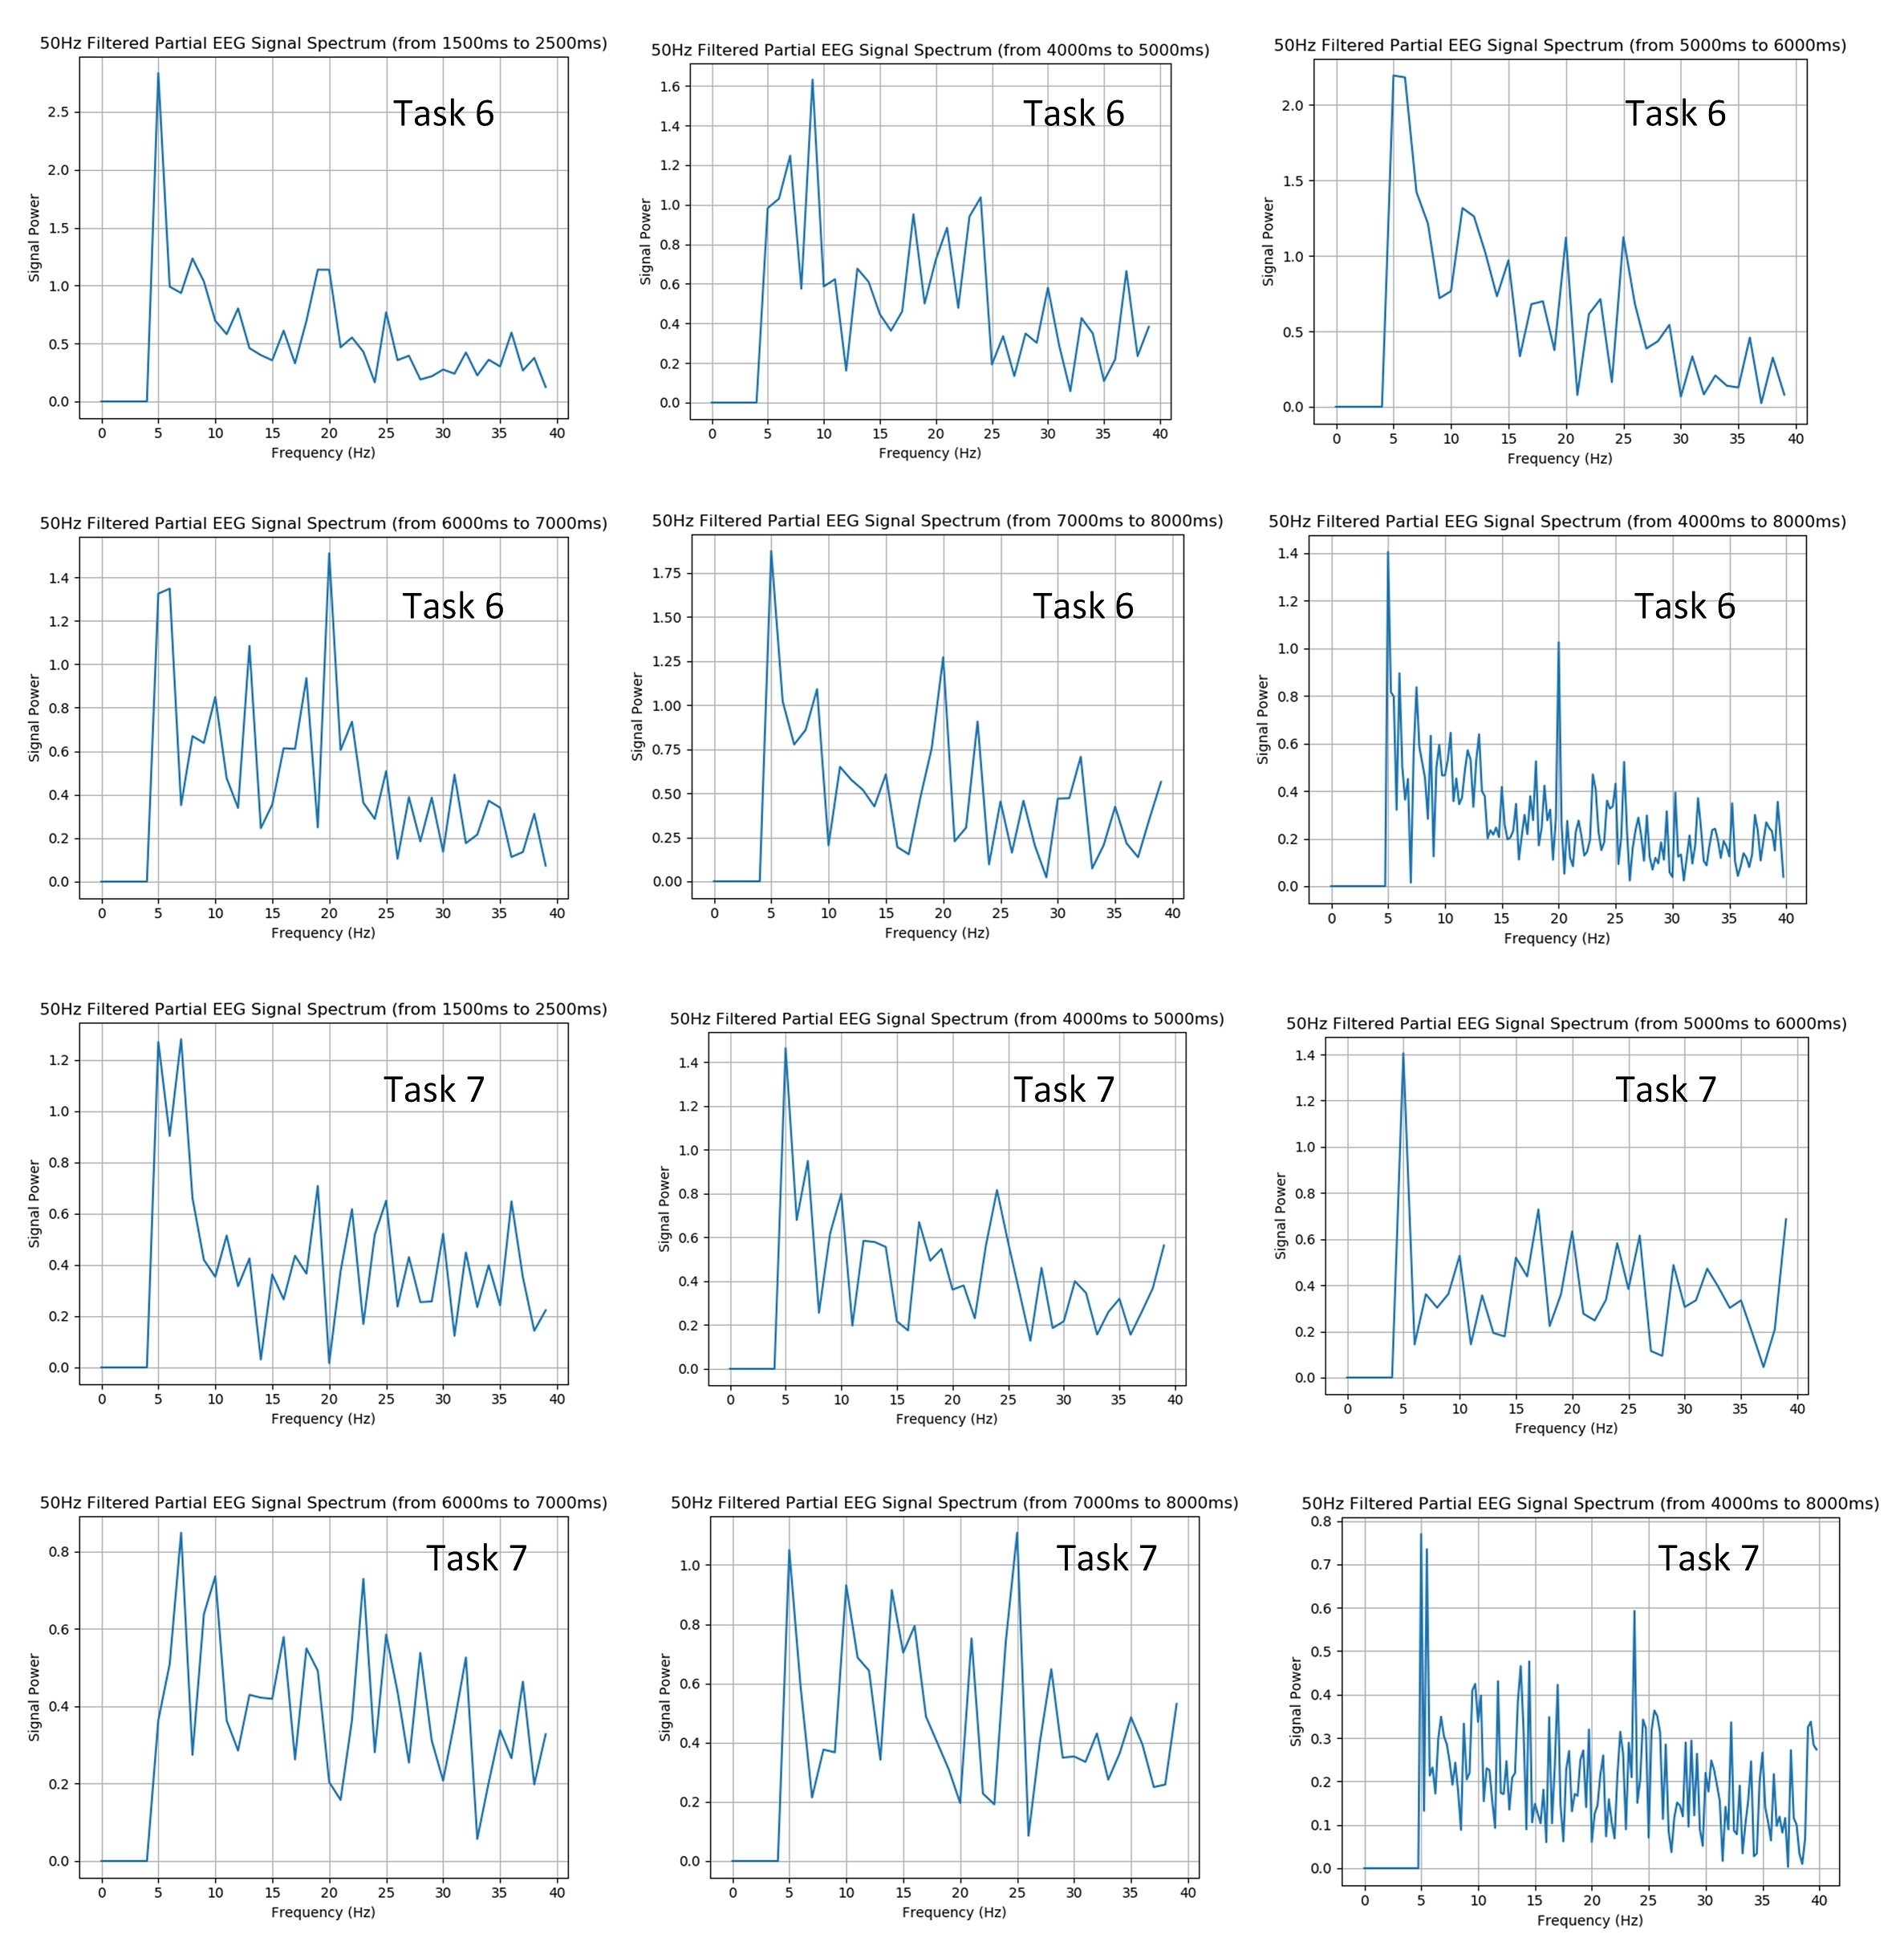
\includegraphics[width=\linewidth]{Figures/Hz102030.jpg} 
%	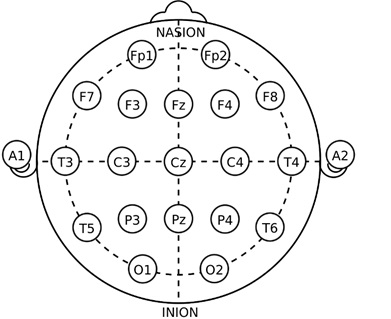
\includegraphics[width=8cm]{Figures/Brain_I20.jpg} 
	\caption{Experiments trying to increase the 20Hz and 30Hz peaks.} 
	\label{Hz2030} 
\end{figure}

\subsection{\bf{Signal-to-Noise Ratio:}}
In order to determine if EEG signals recorded from a single electrode attached on the Fp1 position can be reliable detected, it is necessary to compute the SNR of the recorded EEG signals and then compare them with the SNR Wall. If the EEG signal SNR is greater than the SNR Wall value then the BCI system with a single electrode attached on Fp1 can reliably detect an EEG signal.

The SNR for each signal segment of the recorded EEG signals was calculated using the procedure described in the “Methodology” chapter, where two approaches were described. The first one is based on the ratio of the variance of the conscious signal to the variance of the noise (equation 5). The second approach is based on the noise uncertainty (equation 8). The variances of the noise signal are shown in Table \ref{noise}.

\begin{table}[hbt!]
	\caption{Noise Variance}
	\label{noise}
	\centering
	\begin{tabular}{|c|c|c|l|}
	\hline
		Task &Noise Variancee & Noise Variance Ratio & Effect on SNR calculation\\
		 \hline\hline
		Task1 & 2.07E-08 & 2.05 &	SNR using Eq5 is about 3dB greater than  with Eq.8\\
		Task2 & 4.94E-09 & 0.49 &	SNR using Eq5 is about 3dB less than  with Eq.8\\
		Task3 & 9.56E-09 & 0.95 &	SNR using Eq5 is about the same as that with Eq.8\\
		Task4 & 5.09E-09 & 0.50 &	SNR using Eq5 is about 3dB less than  with Eq.8\\
		Task5 & 9.49E-09 & 0.94 &	SNR using Eq5 is about the same as that with Eq.8\\
		Task6 & 1.52E-08 & 1.50 &	SNR using Eq5 is about 1.75dB greater than  with Eq.8\\
		Task7 & 9.49E-09 & 0.94 &	SNR using Eq5 is about the same as that with Eq.8\\
		 \hline
	\end{tabular}
\end{table}


The maximum noise variance is the noise variance for Task1, while the minimum is the variance of Task2. The noise uncertainty (\textrho) is equal to 2.05 as computed with equation 6, while the overall noise variance is 1.01E-08 (computed with equation 7). Therefore, to compute the SNR using equation 5, the noise variance to be used is the one shown in table 2. To compute the SNR using equation 8, the noise variance to be used is for all tasks 1.01E-08. This will result in a change in the SNR given in table \ref{noise}. This can be verified by the plots of the SNR for all signal segments for the case of Task1 and Task3. From in Figure \ref{SNRdiff}, it can be seen that for the case of Task 1 there is a difference of about 3dB between the SNR computed with eq. 5. (series2) and the SNR computed with eq. 8. In the case of Task 3 the SNR is almost the same between the two methods. 


\begin{figure}%[hbt!]
	\centering
%	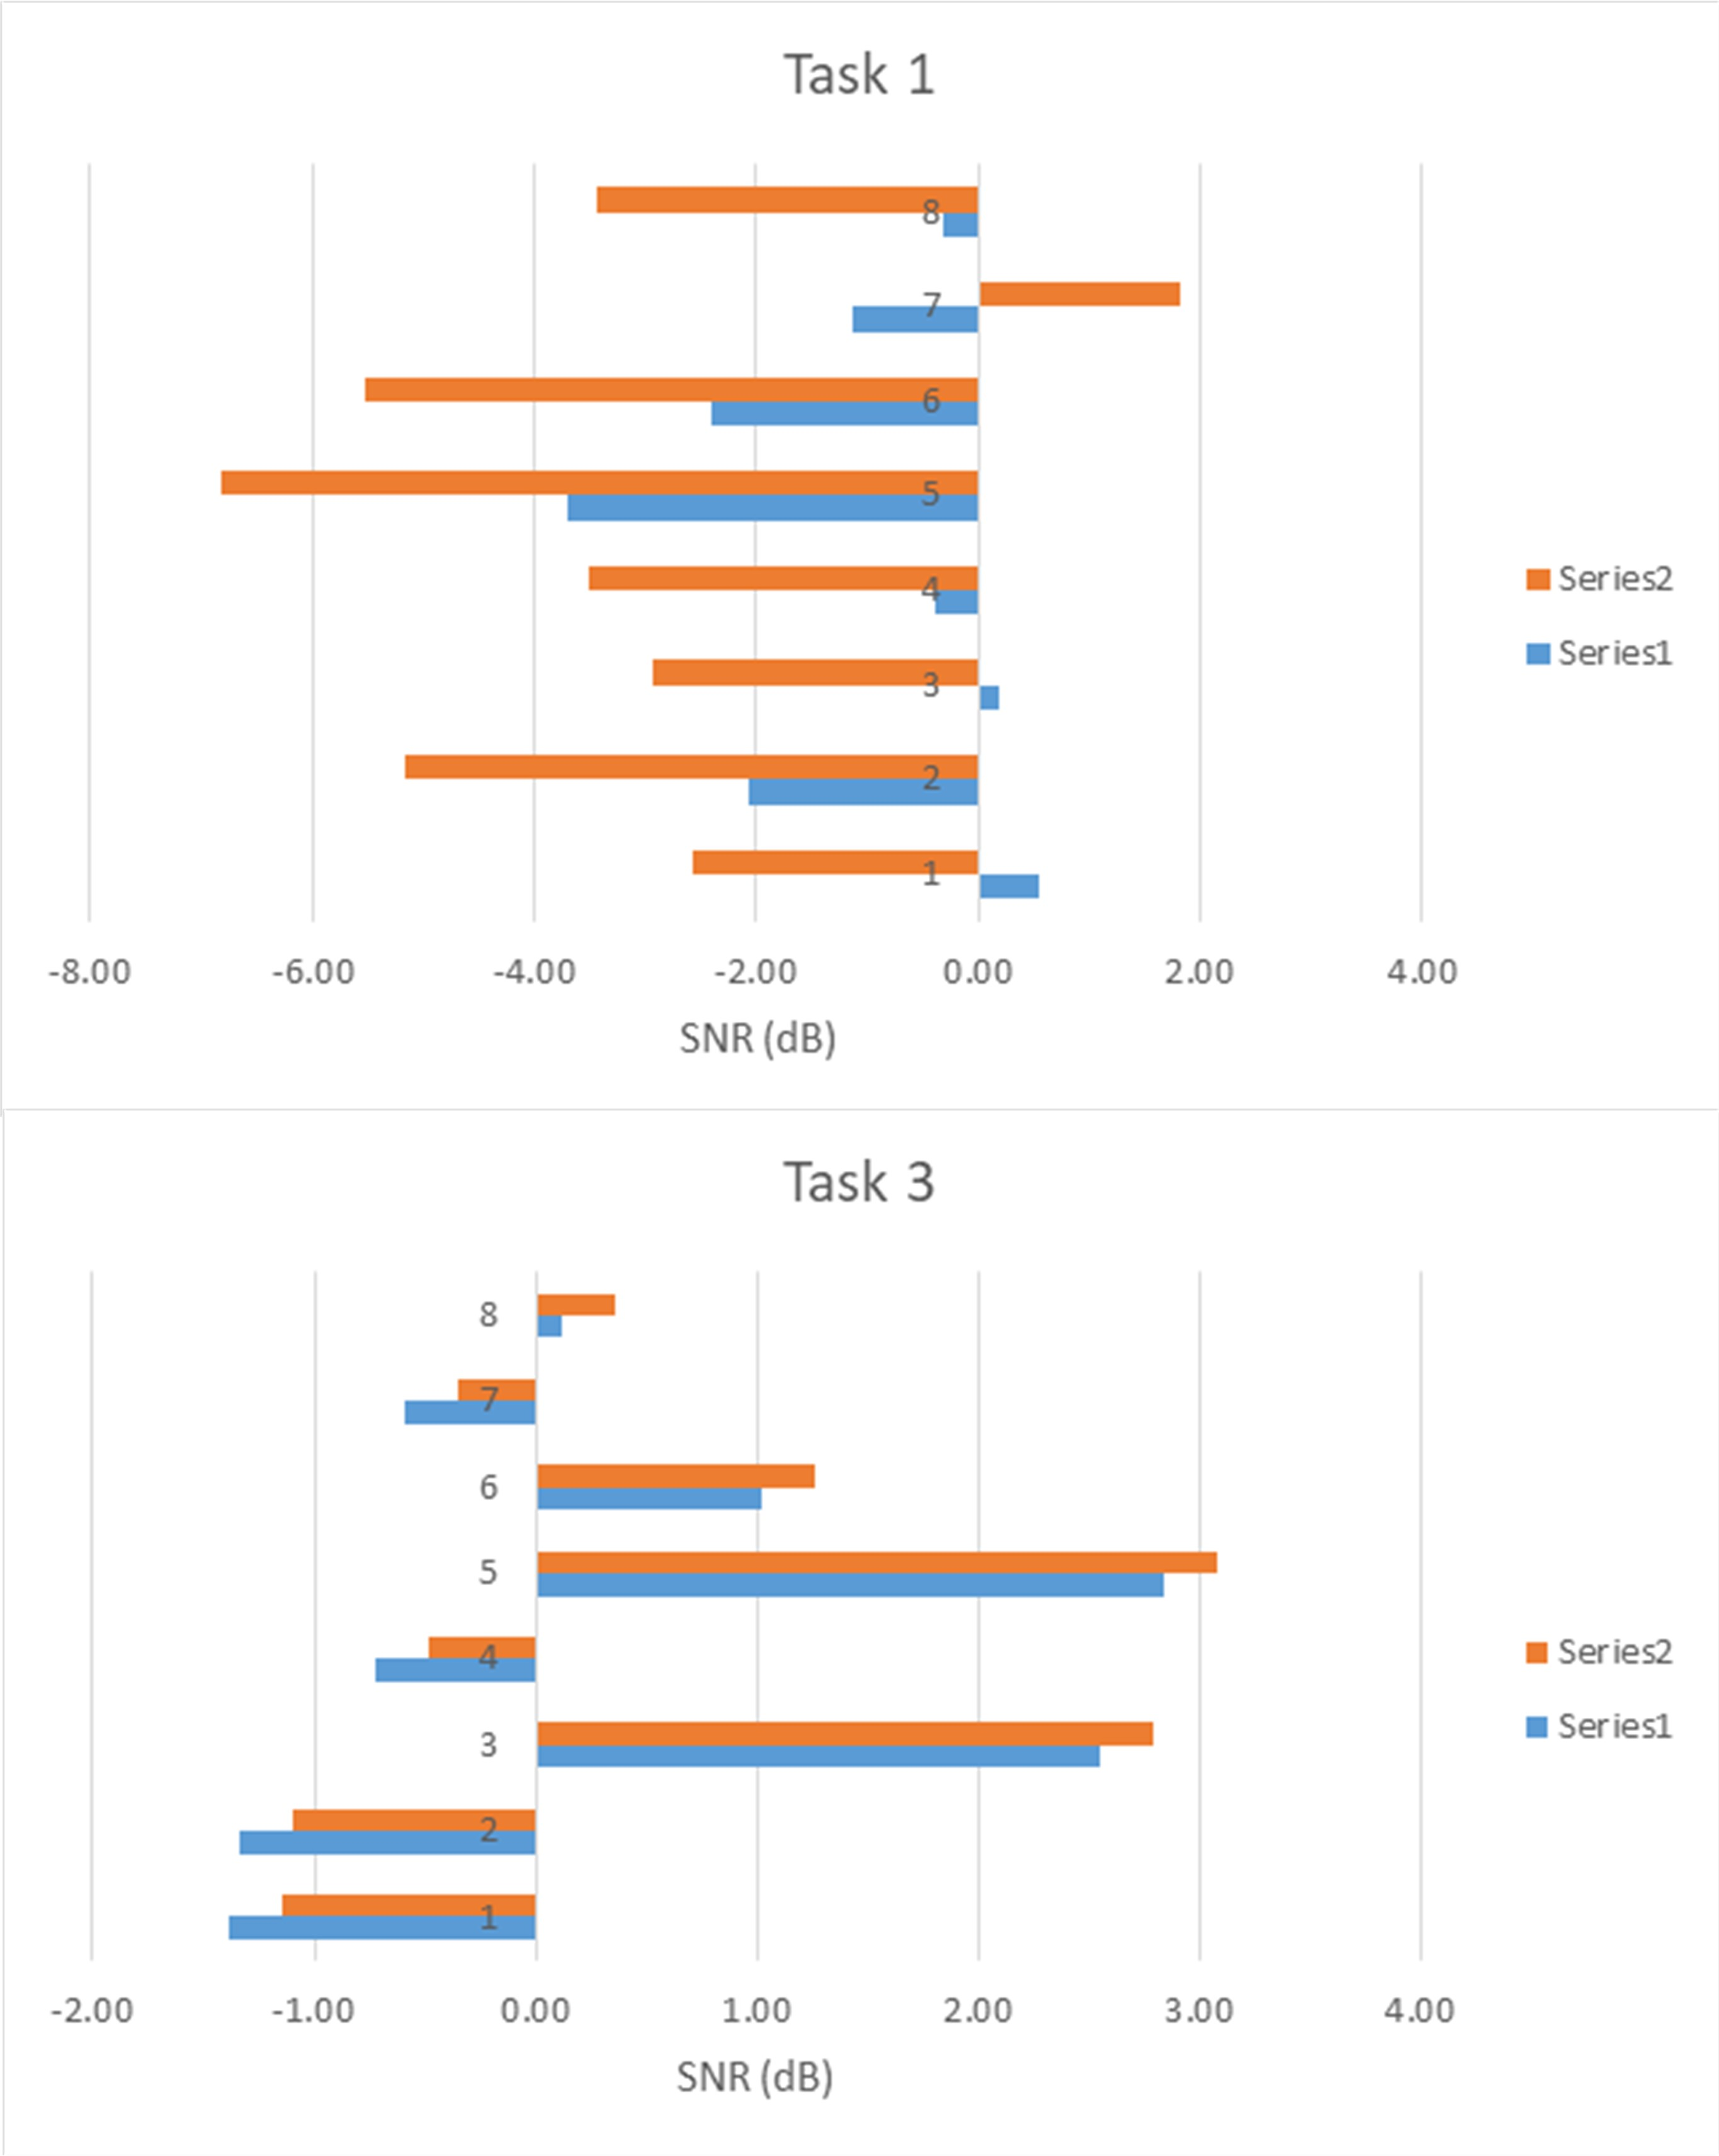
\includegraphics[width=\linewidth]{Figures/SNRchange.jpg} 
	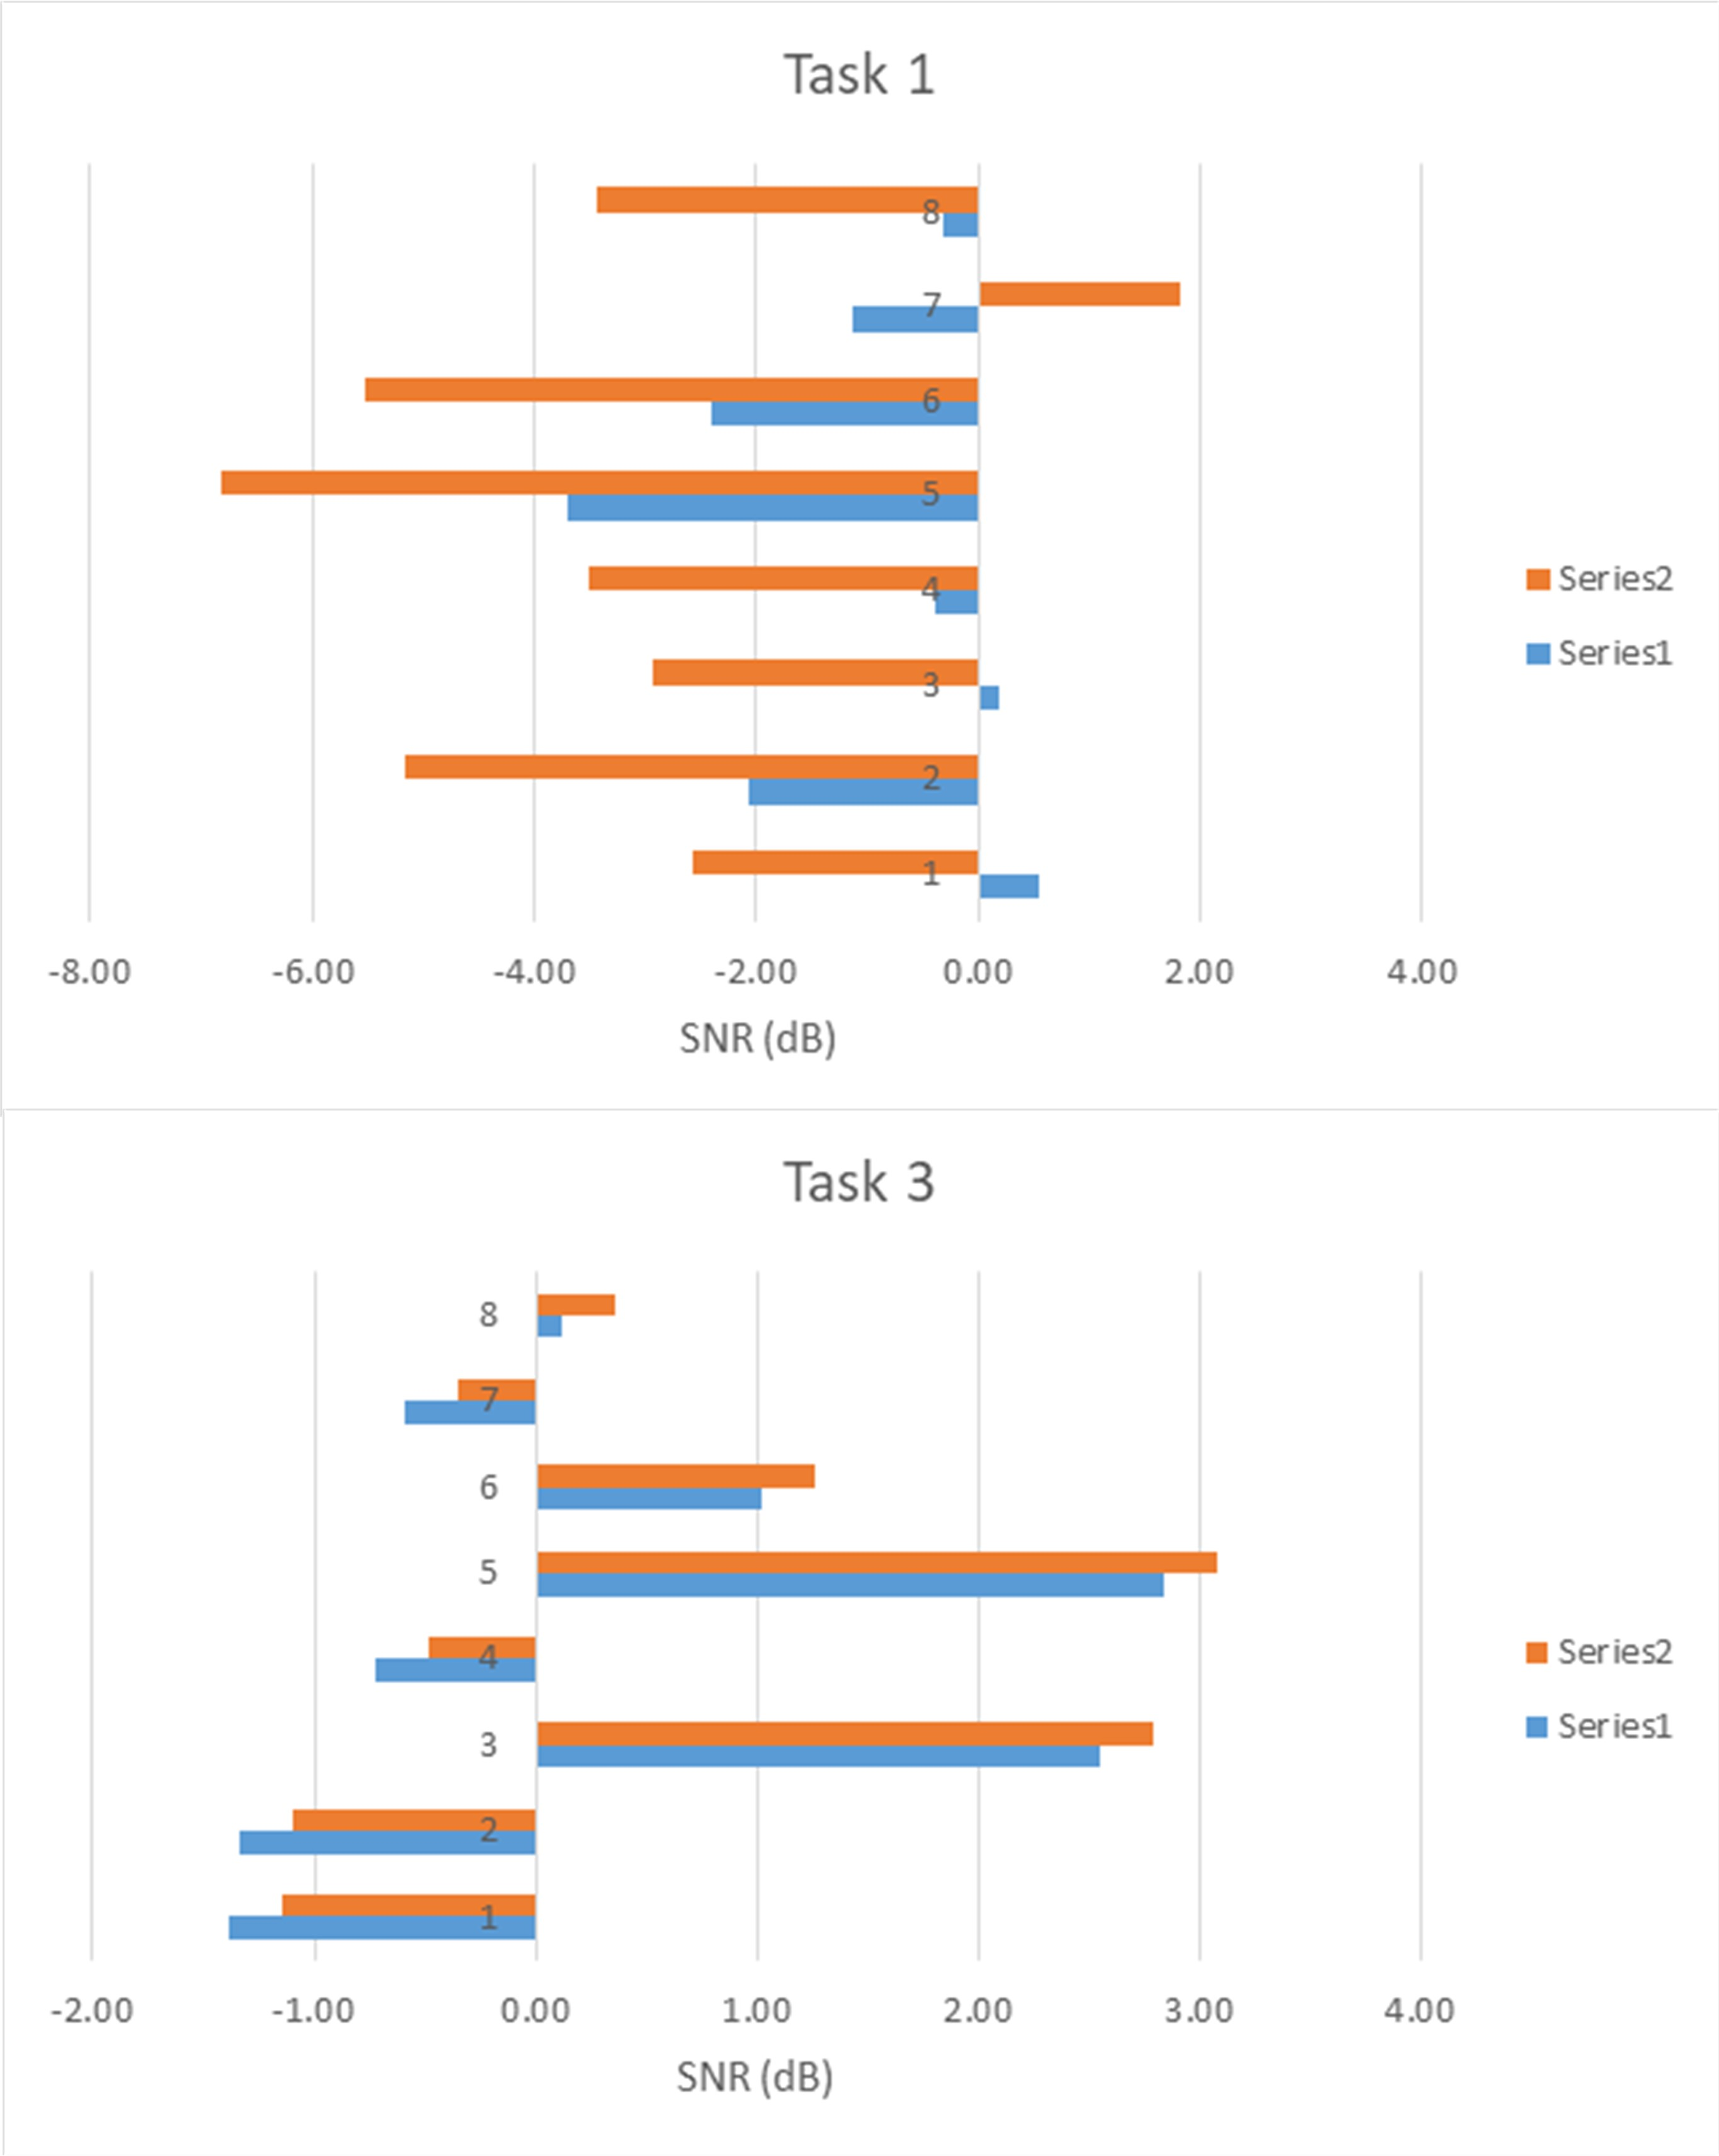
\includegraphics[width=9cm]{Figures/SNRchange.jpg} 
	\caption{SNR Difference when using Eq. 5 and Eq. 8.} 
	\label{SNRdiff} 
\end{figure}

The SNR was calculated for each signal segment. The calculated SNR values are given in Table \ref{SNRall}. Signal segments 1 to 7 correspond to the signal segments recorded during the time intervals 4s to 5s, 4.5s to 5.5s, 5s to 6s, 5.5s to 6.5s etc. The last column (column 8) corresponds to the segment for 4s to 8s.


\begin{table}[hbt!]
	\caption{ SNR for all Experiments}
	\label{SNRall}
	\centering
	\begin{tabular}{|c|c|c|c|c|c|c|c|c|}
	\hline
		%Signal Segment
		%hline
		Task & Segm. 1 & Segm. 2 & Segm. 3 & Segm. 4 & Segm. 5 & Segm. 6 & Segm. 7 & Segm. 8\\
		 \hline\hline
		%\vspace {3pt}
		Task1 &0.55 & -2.06	 &0.19 & -0.39  & 3.71 & -2.41 & -1.14 & -0.32\\
		%\vspace{3pt}
		\hline
		Task2 &1.02 & -0.61	 & -1.00 &	-1.15 & -5.01 & 	-0.64 & -1.97 & 	-0.34\\
		\hline
		Task3 & -1.38 &	 -1.34 & 2.55 & -0.72 & 2.84 & 1.02 & -0.59 & 0.11\\
		\hline
		Task4 & -3.01 &	 1.27	 & -1.08 & 0.28 & -3.05 & -3.44 & -1.82 & -0.35\\
		\hline
		Task5 & -0.71 &	 -1.00 & -2.21 & 0.10 & -0.35 & -1.73 & 0.69 & -0.88\\
		\hline
		Task6 & 3.38 &	-1.03	 & -0.97 & 0.86 & -0.35 & -0.51 & 0.69 & 0.96\\
		\hline
		Task7 &-0.71 &	-1.00 & -2.21 &	0.10 & -0.35 & -1.73 & 0.69 & -0.88\\
		 \hline
	\end{tabular}
\end{table}


The SNR for each experiment plots are shown separately in Figures \ref{SNR1} to \ref{SNR7} . These are computed using Eq. 8. On each one of these plots the values for the SNR walls are taken from (Porr B. , 2018), for three of the scenarios used (relaxed, eye blinking and solving Sudoku). The values used are the ones determined with the filter parameters EEG 8Hz to 18Hz, band pass 4Hz to 35Hz and noise reduction 1. The reason for choosing these SNR wall cases is because when using a BCI system the user will operate in a fashion similar to the Sudoku solving process. When using a BCI system, a common source of artefacts is due to eye blinking, because in most cases this is done unintentionally. The relaxed SNR wall is included as a reference because the SNR is computed using the relaxed EEG signals as the noise reference. 

\begin{figure}[hbt!]
	\centering
%	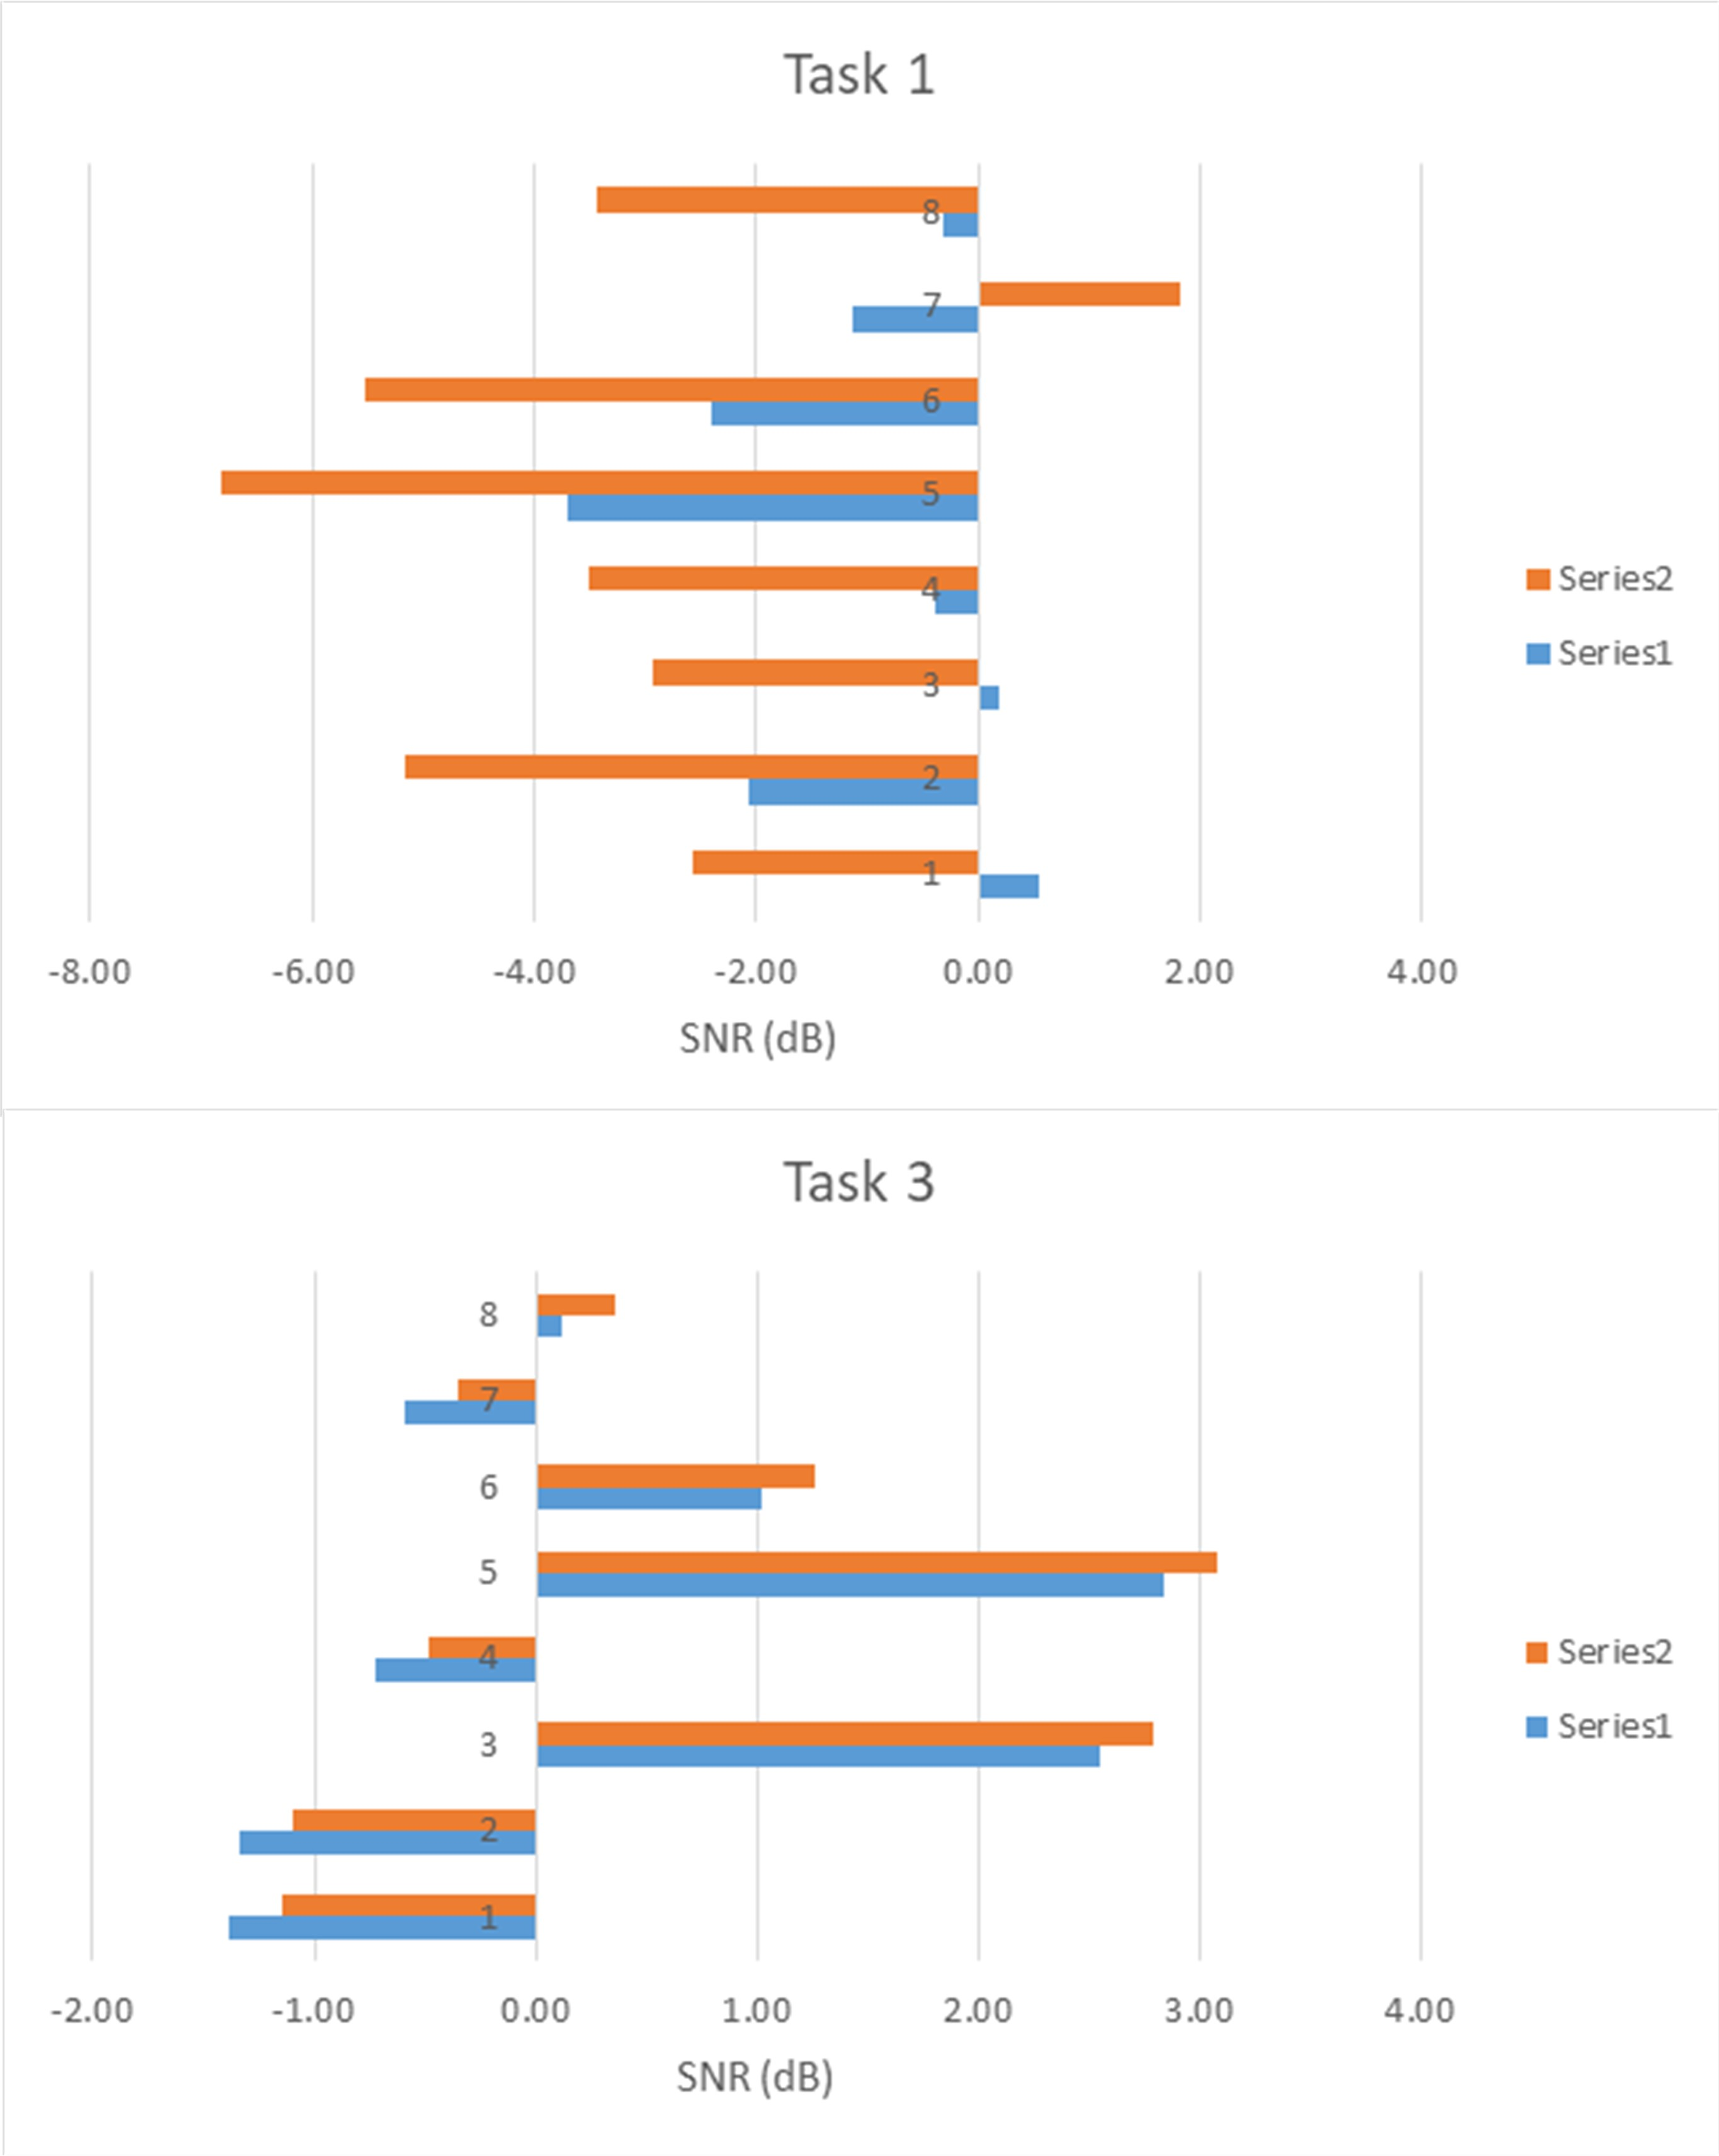
\includegraphics[width=\linewidth]{Figures/SNRchange.jpg} 
	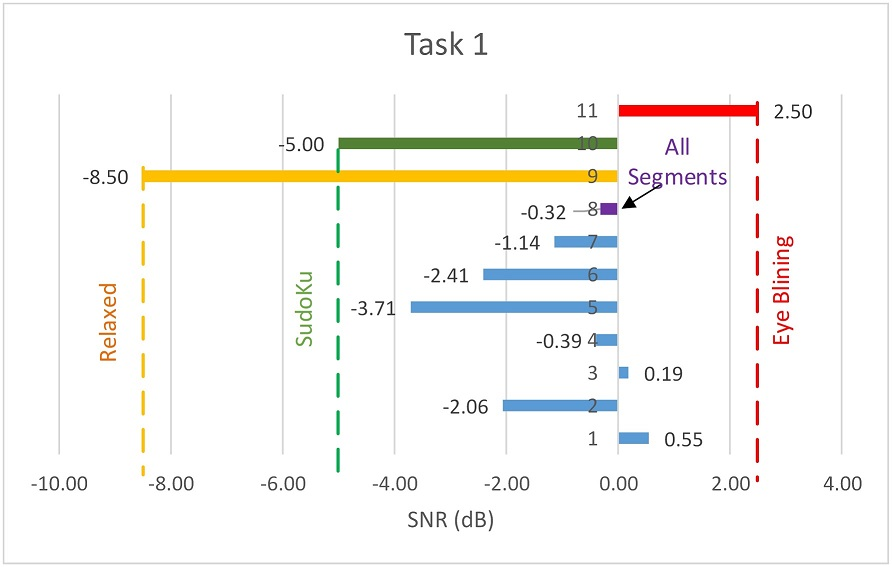
\includegraphics[width=10cm]{Figures/SNRtask1.jpg} 
	\caption{SNR for Task1.} 
	\label{SNR1} 
\end{figure}

\begin{figure}[hbt!]
	\centering
%	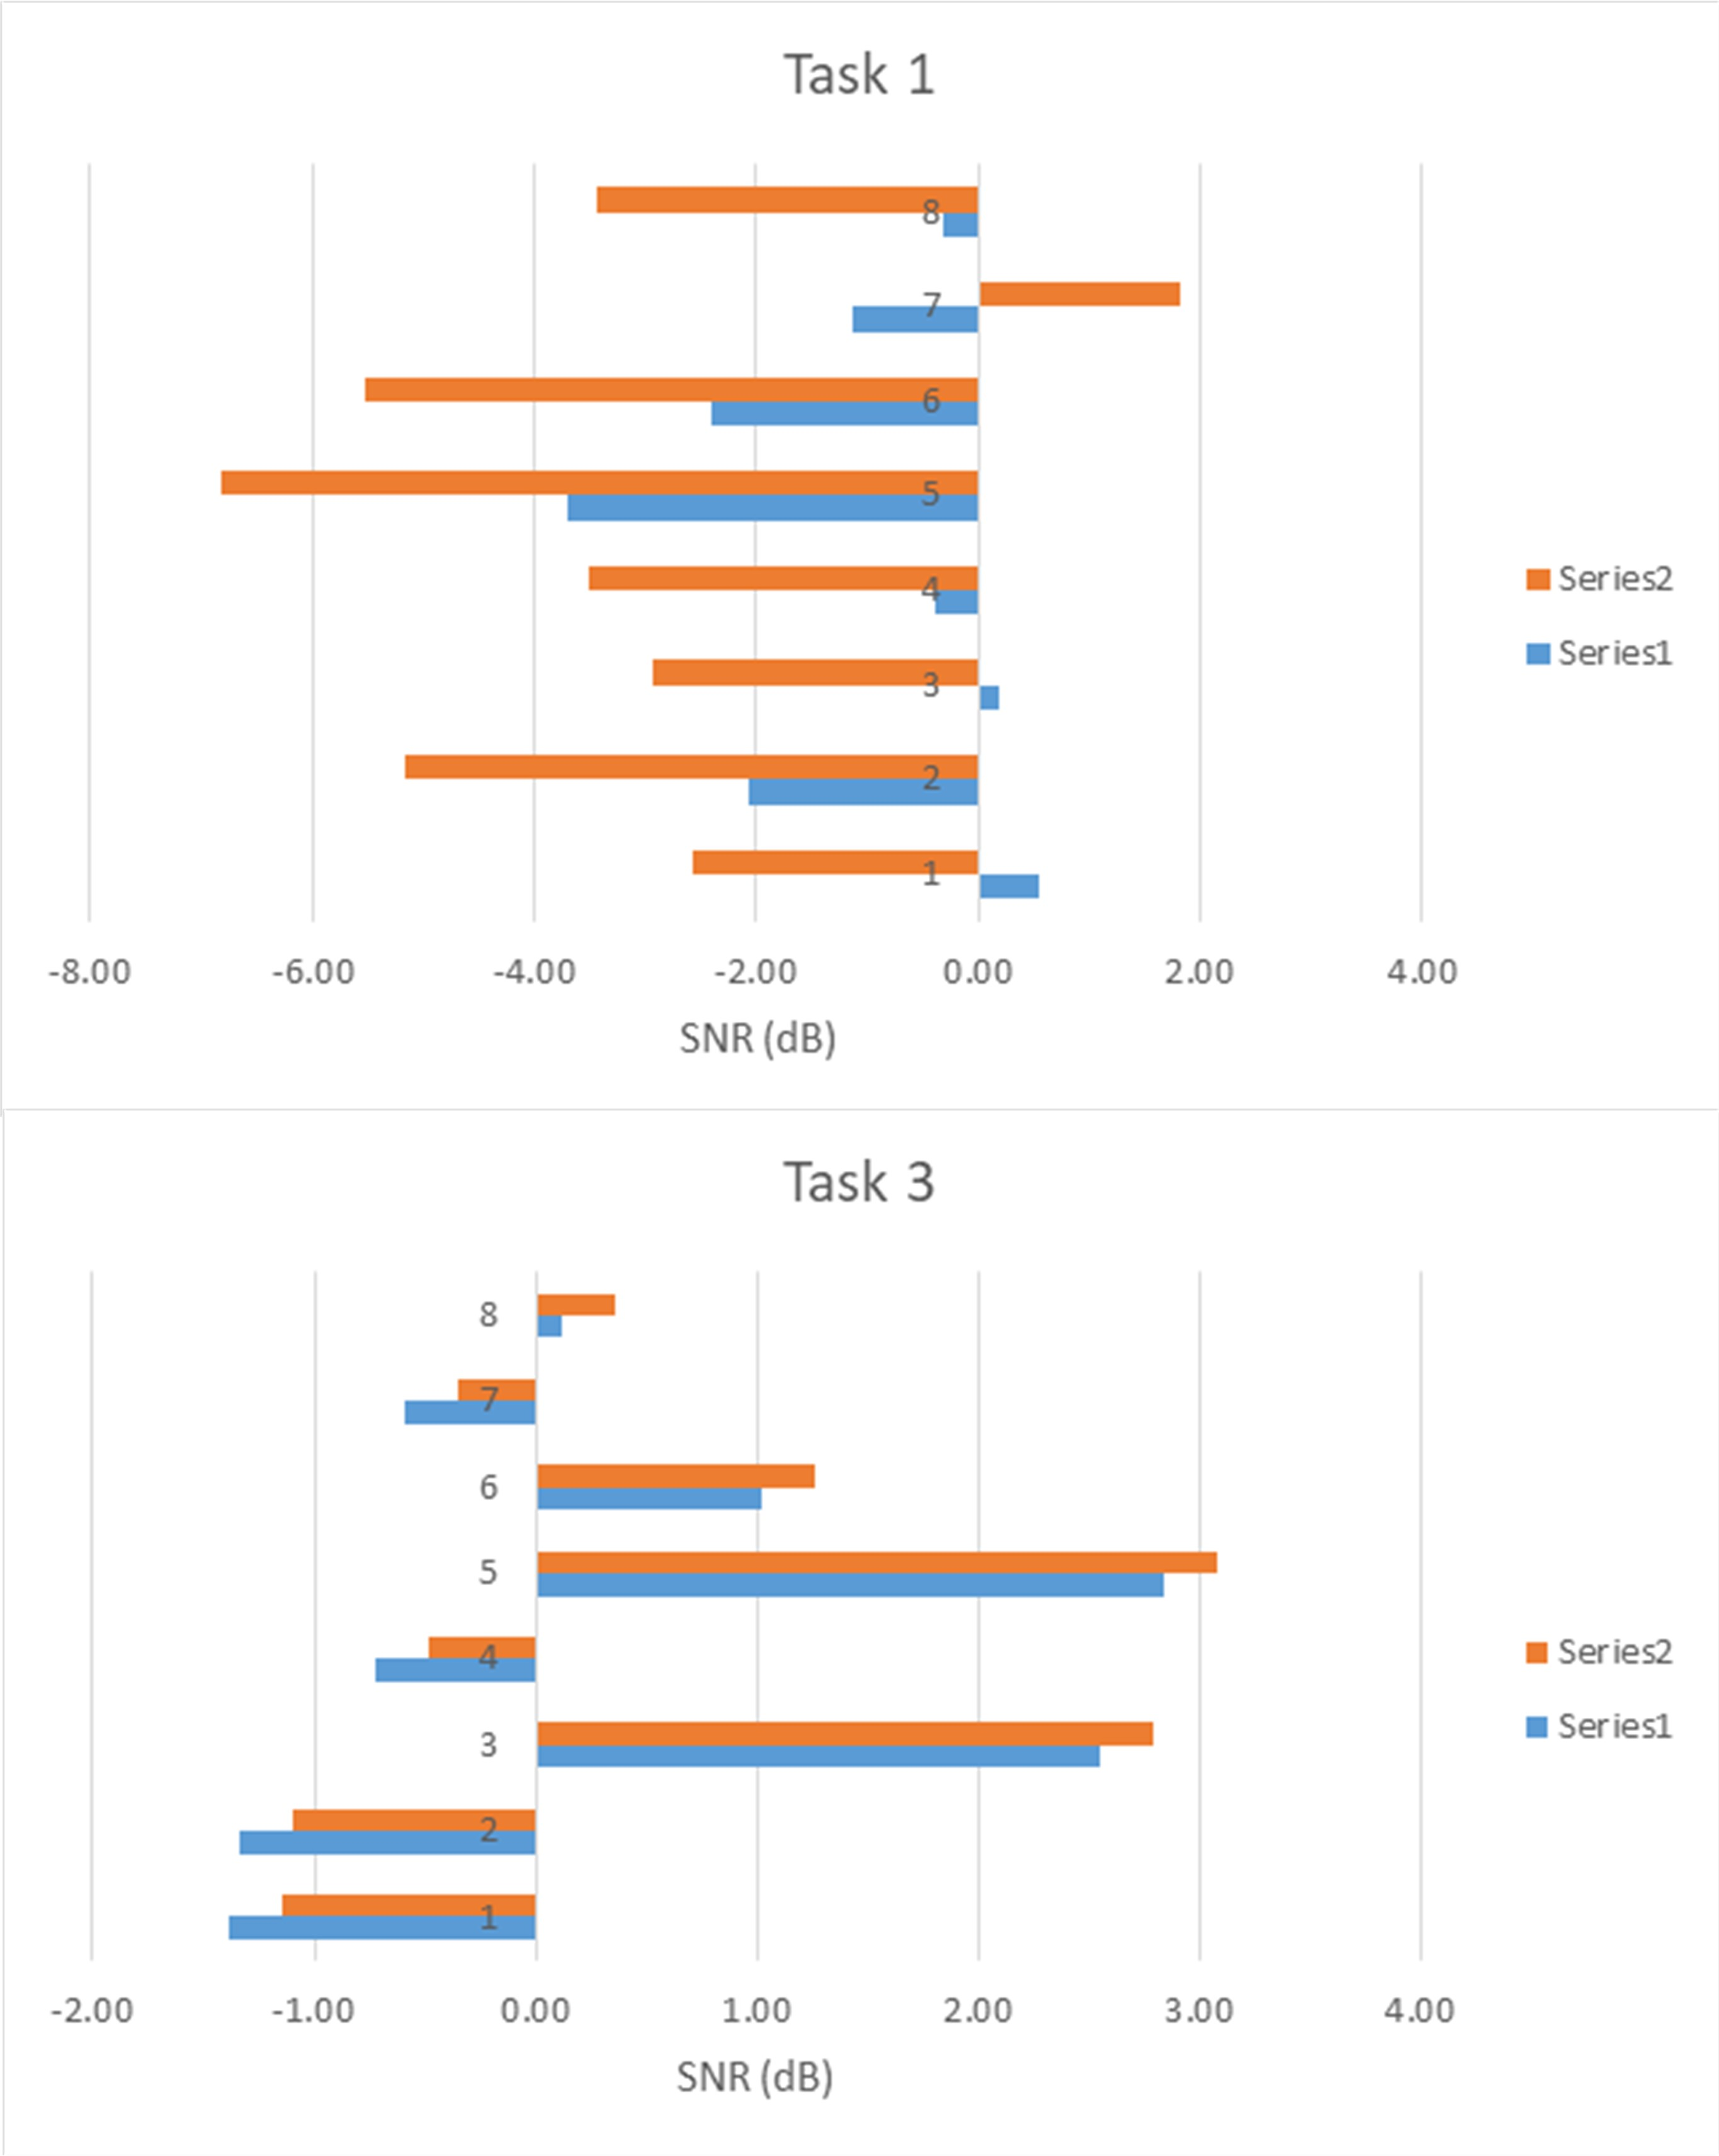
\includegraphics[width=\linewidth]{Figures/SNRchange.jpg} 
	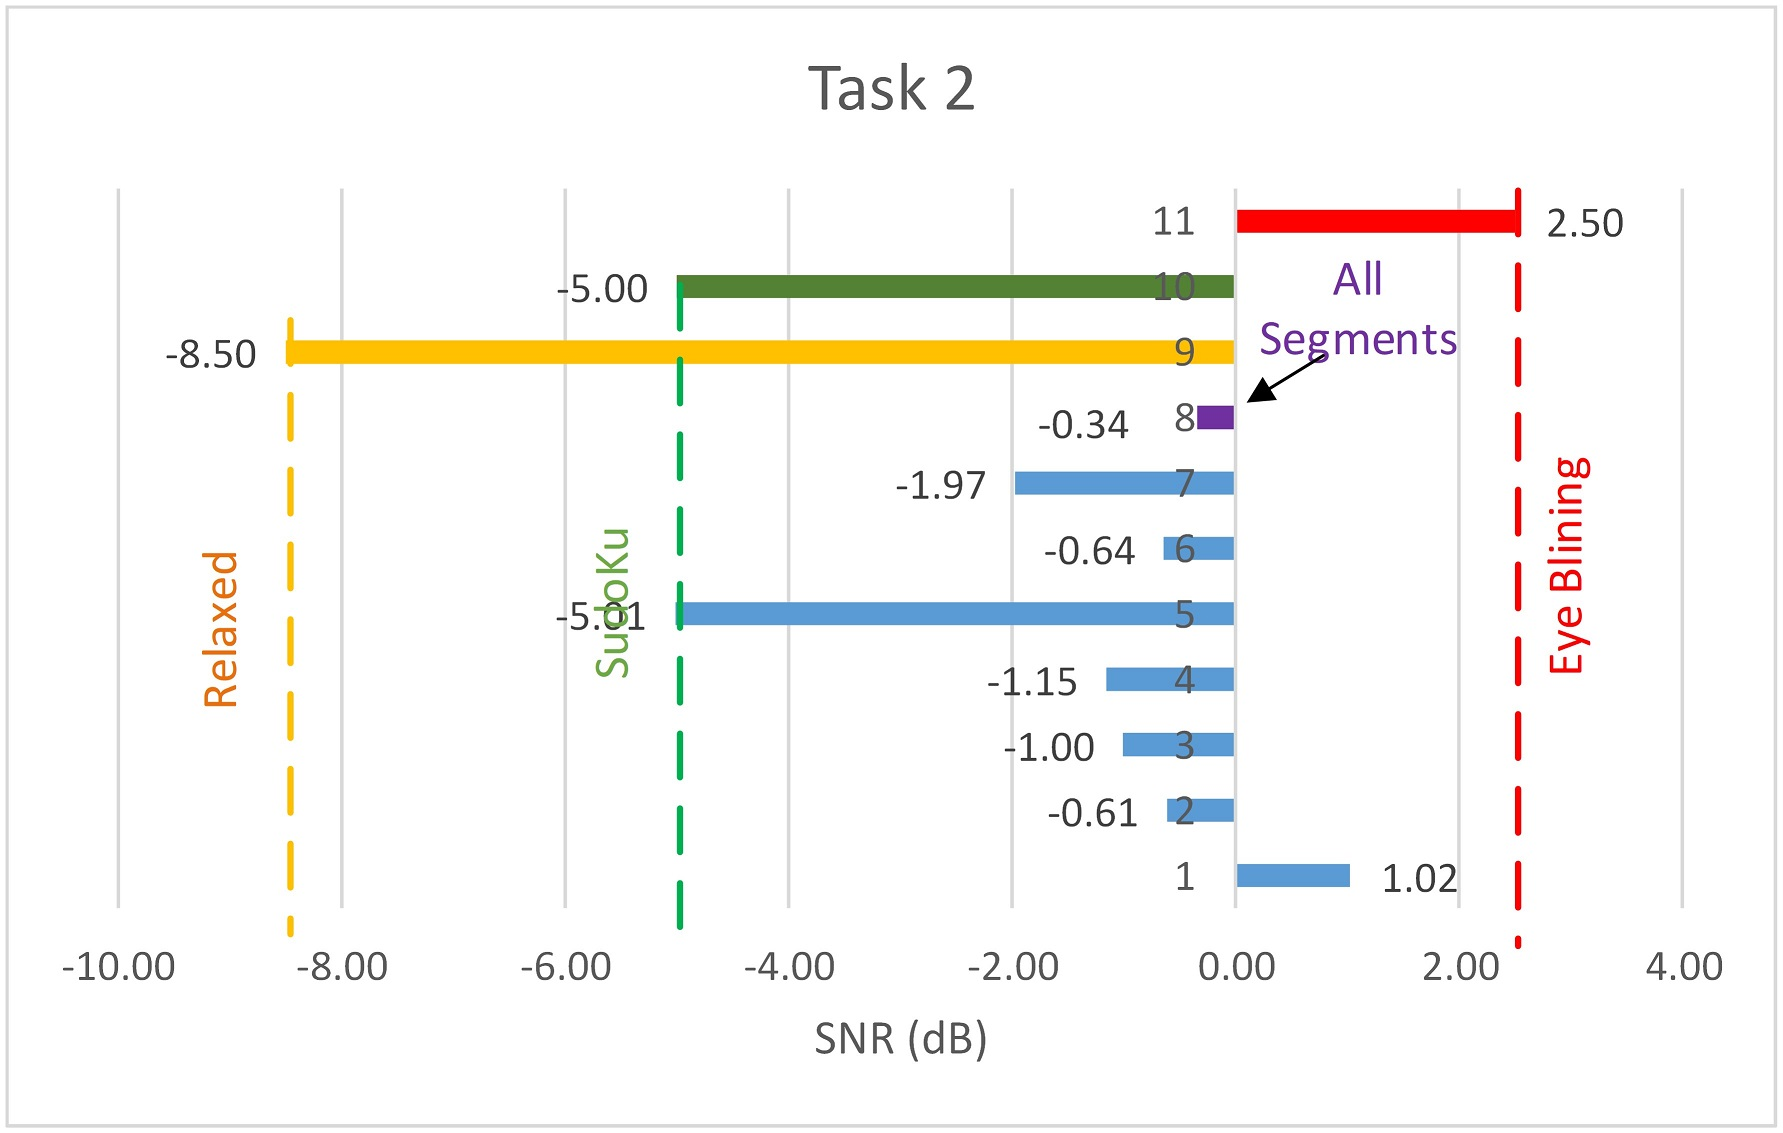
\includegraphics[width=10cm]{Figures/SNRtask2.jpg} 
	\caption{SNR for Task2.} 
	\label{SNR2} 
\end{figure}

\begin{figure}[hbt!]
	\centering
%	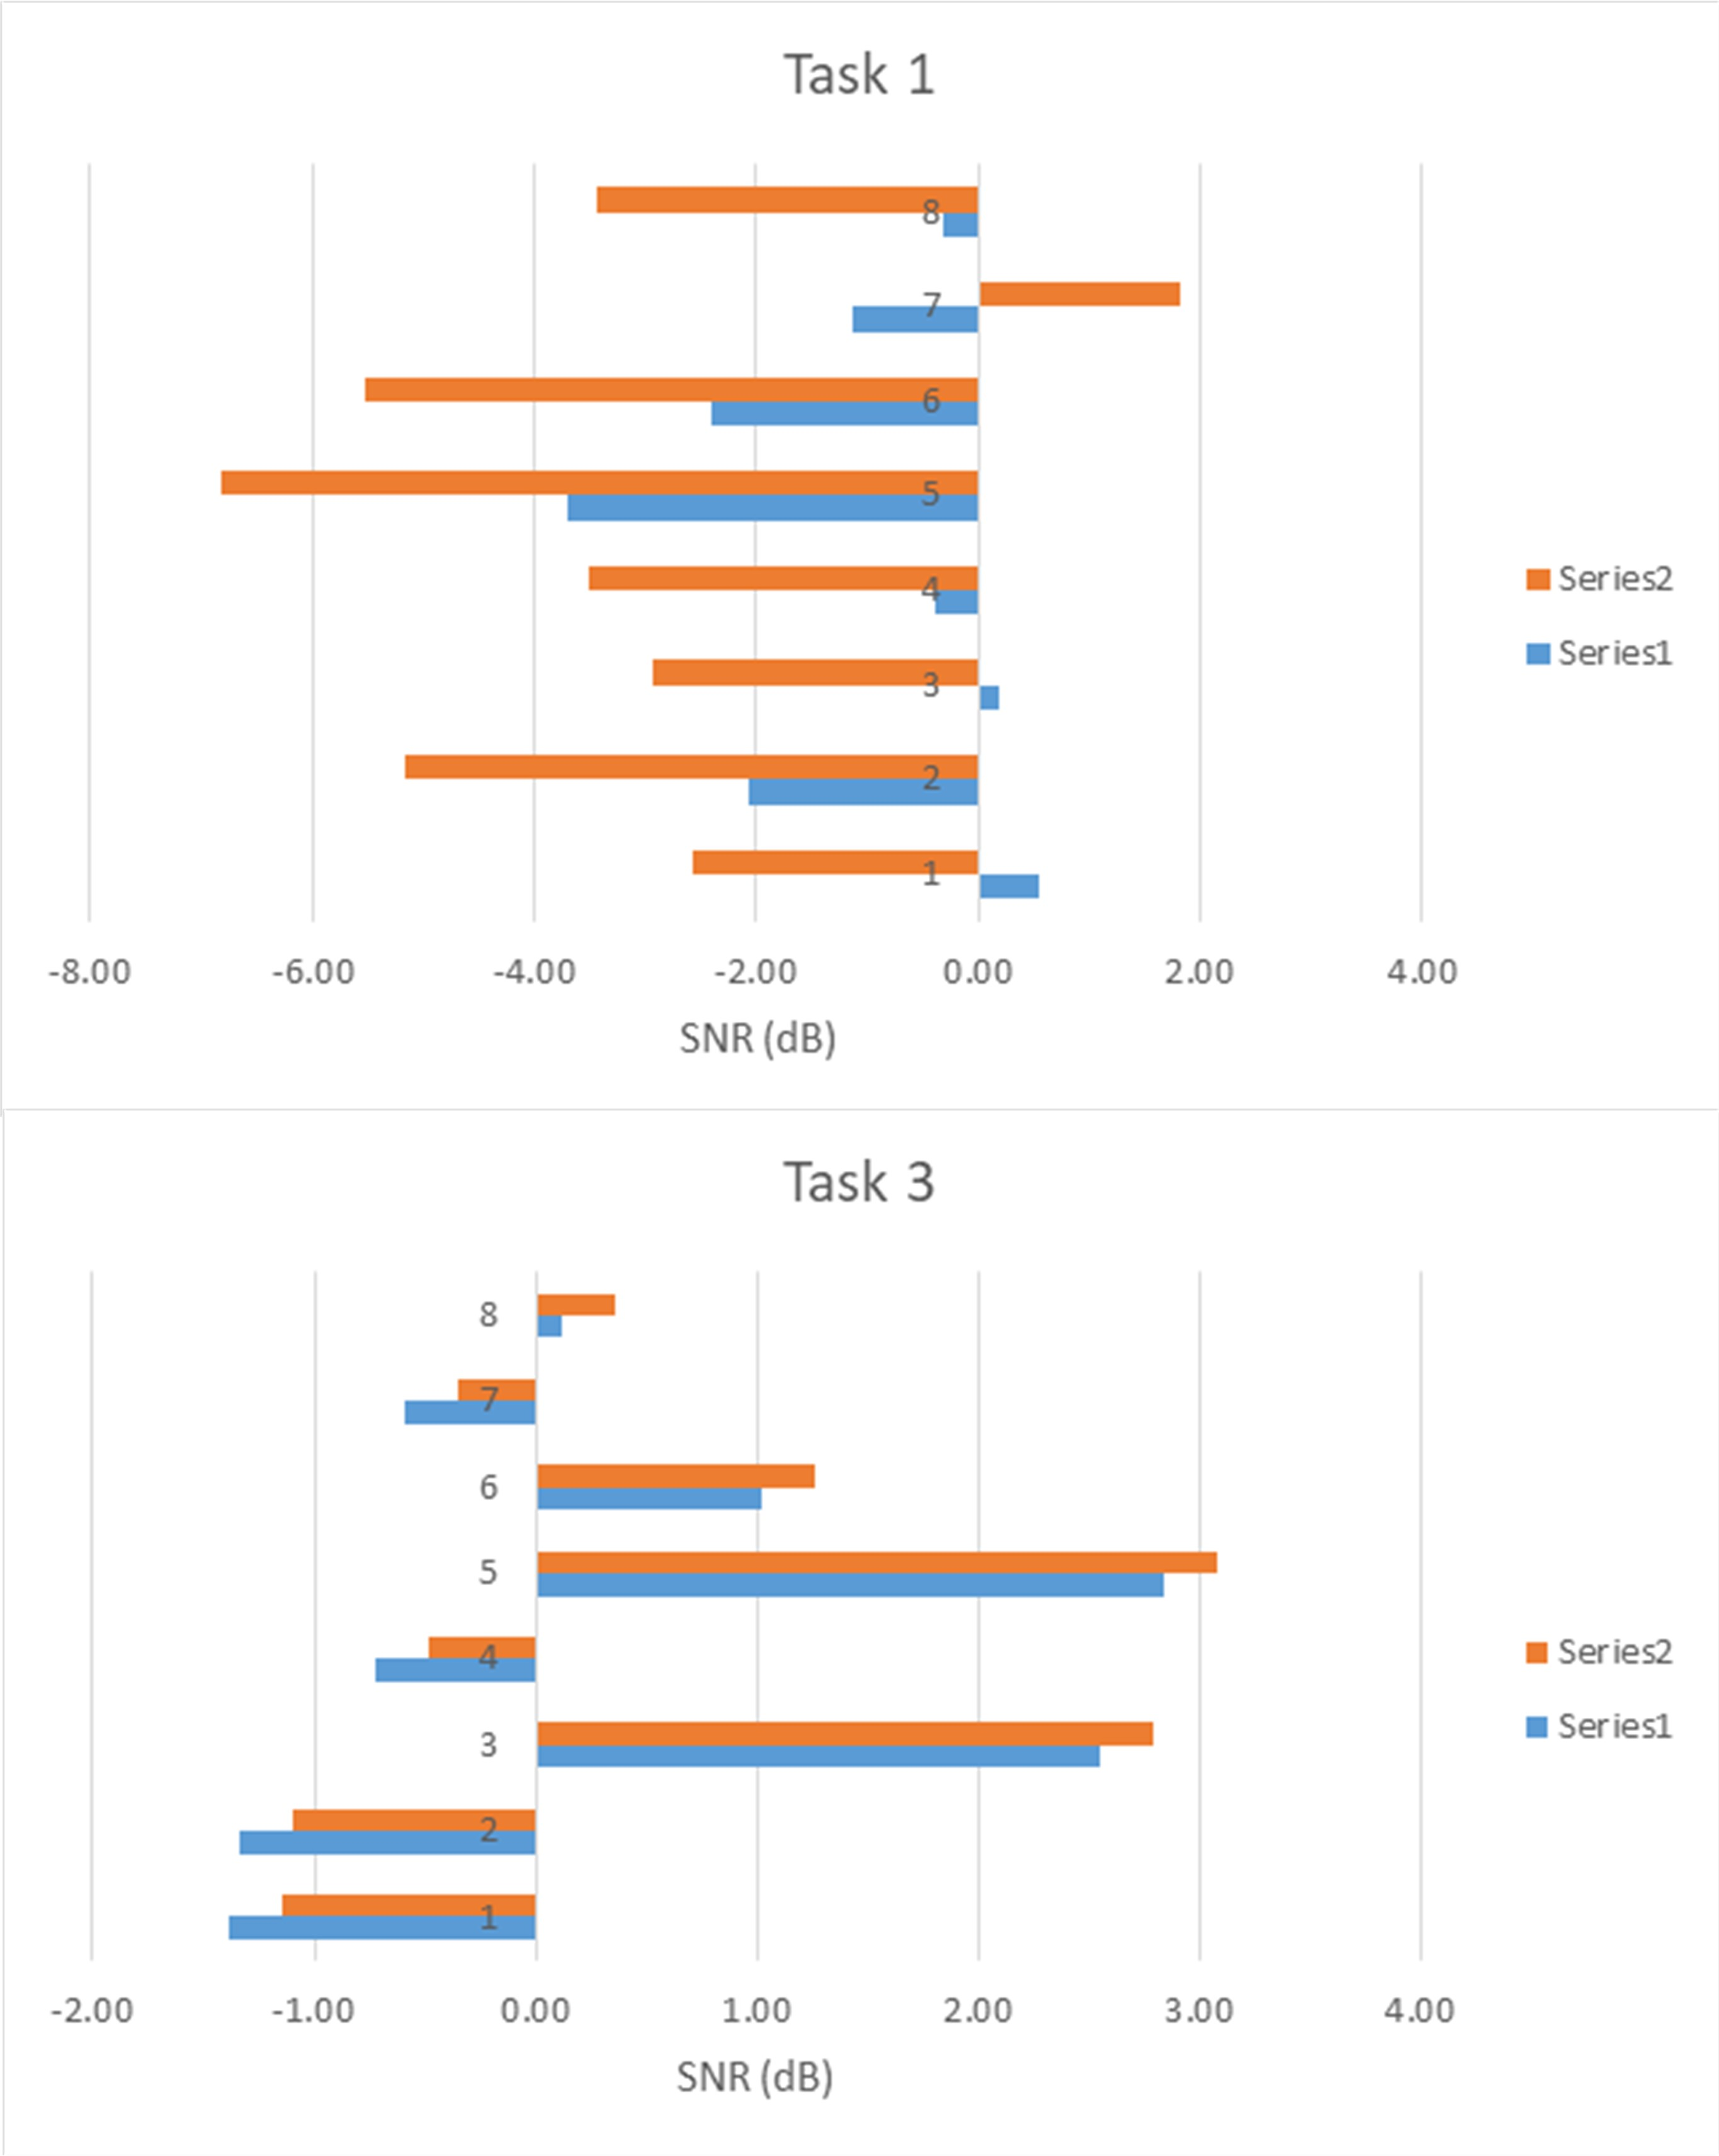
\includegraphics[width=\linewidth]{Figures/SNRchange.jpg} 
	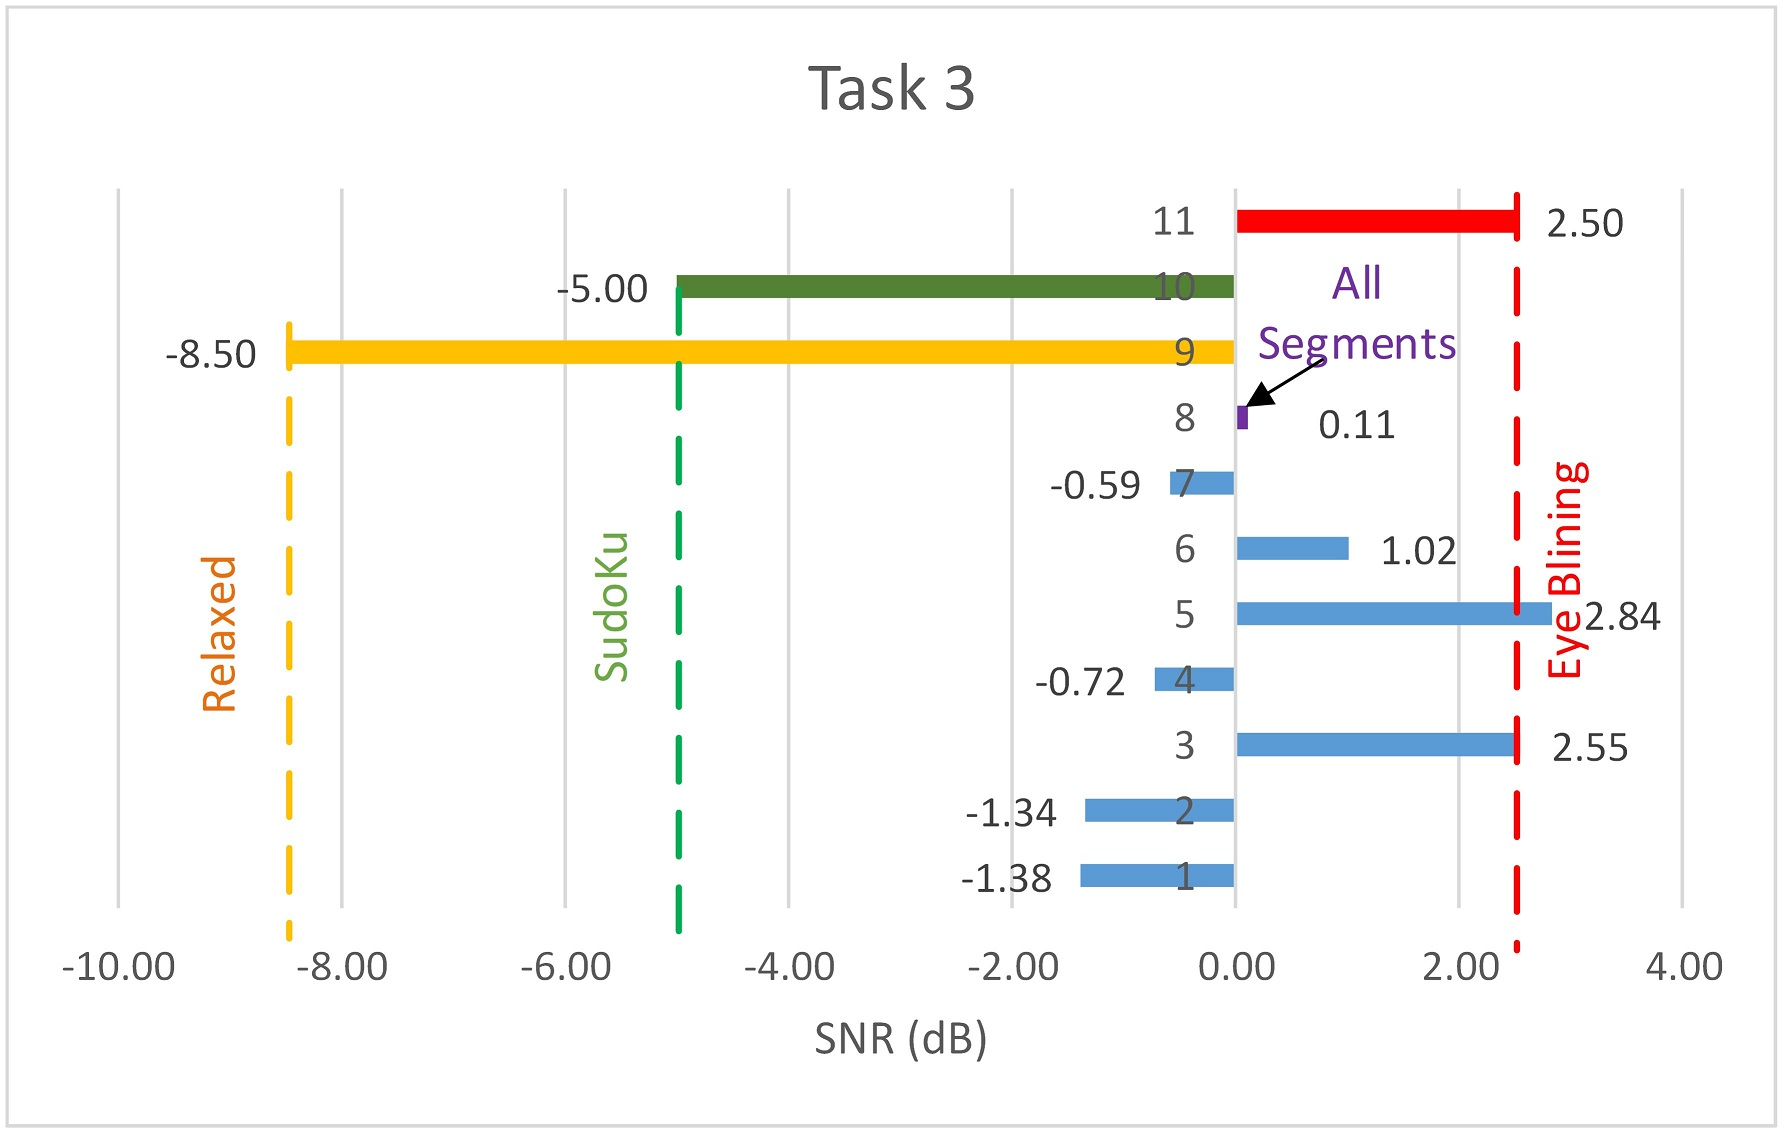
\includegraphics[width=10cm]{Figures/SNRtask3.jpg} 
	\caption{SNR for Task3.} 
	\label{SNR3} 
\end{figure}


\begin{figure}[hbt!]
	\centering
%	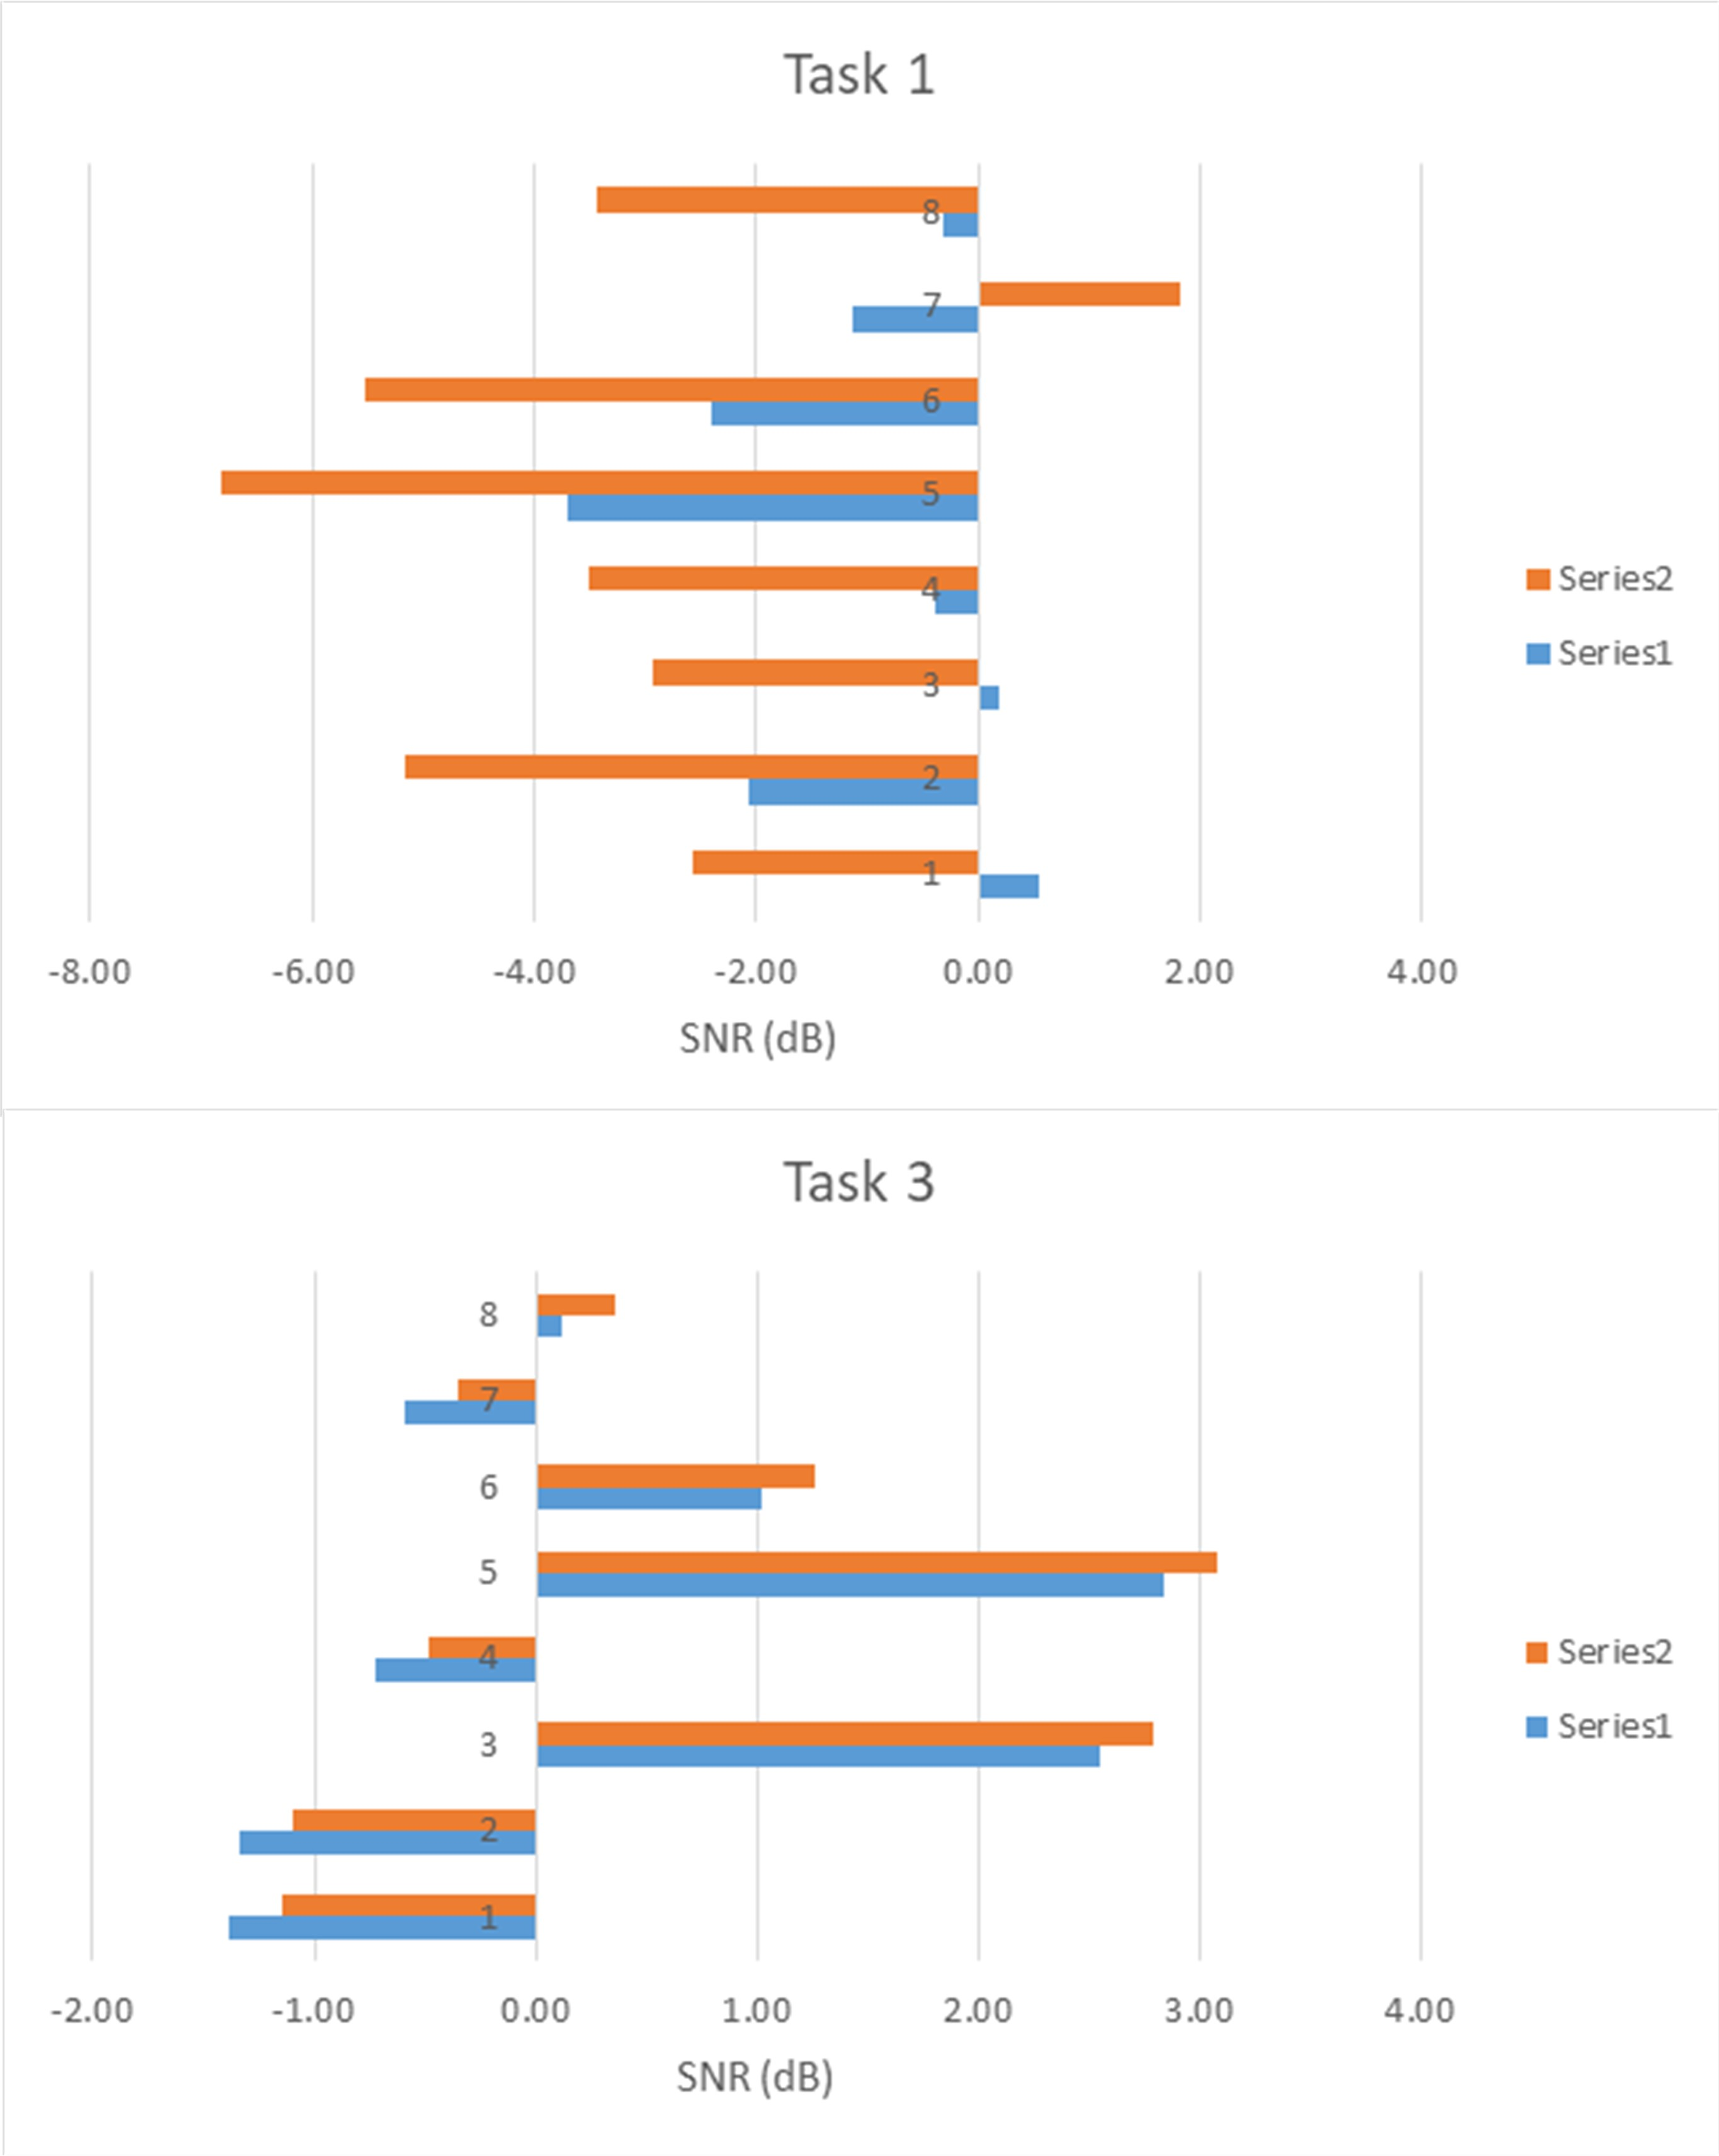
\includegraphics[width=\linewidth]{Figures/SNRchange.jpg} 
	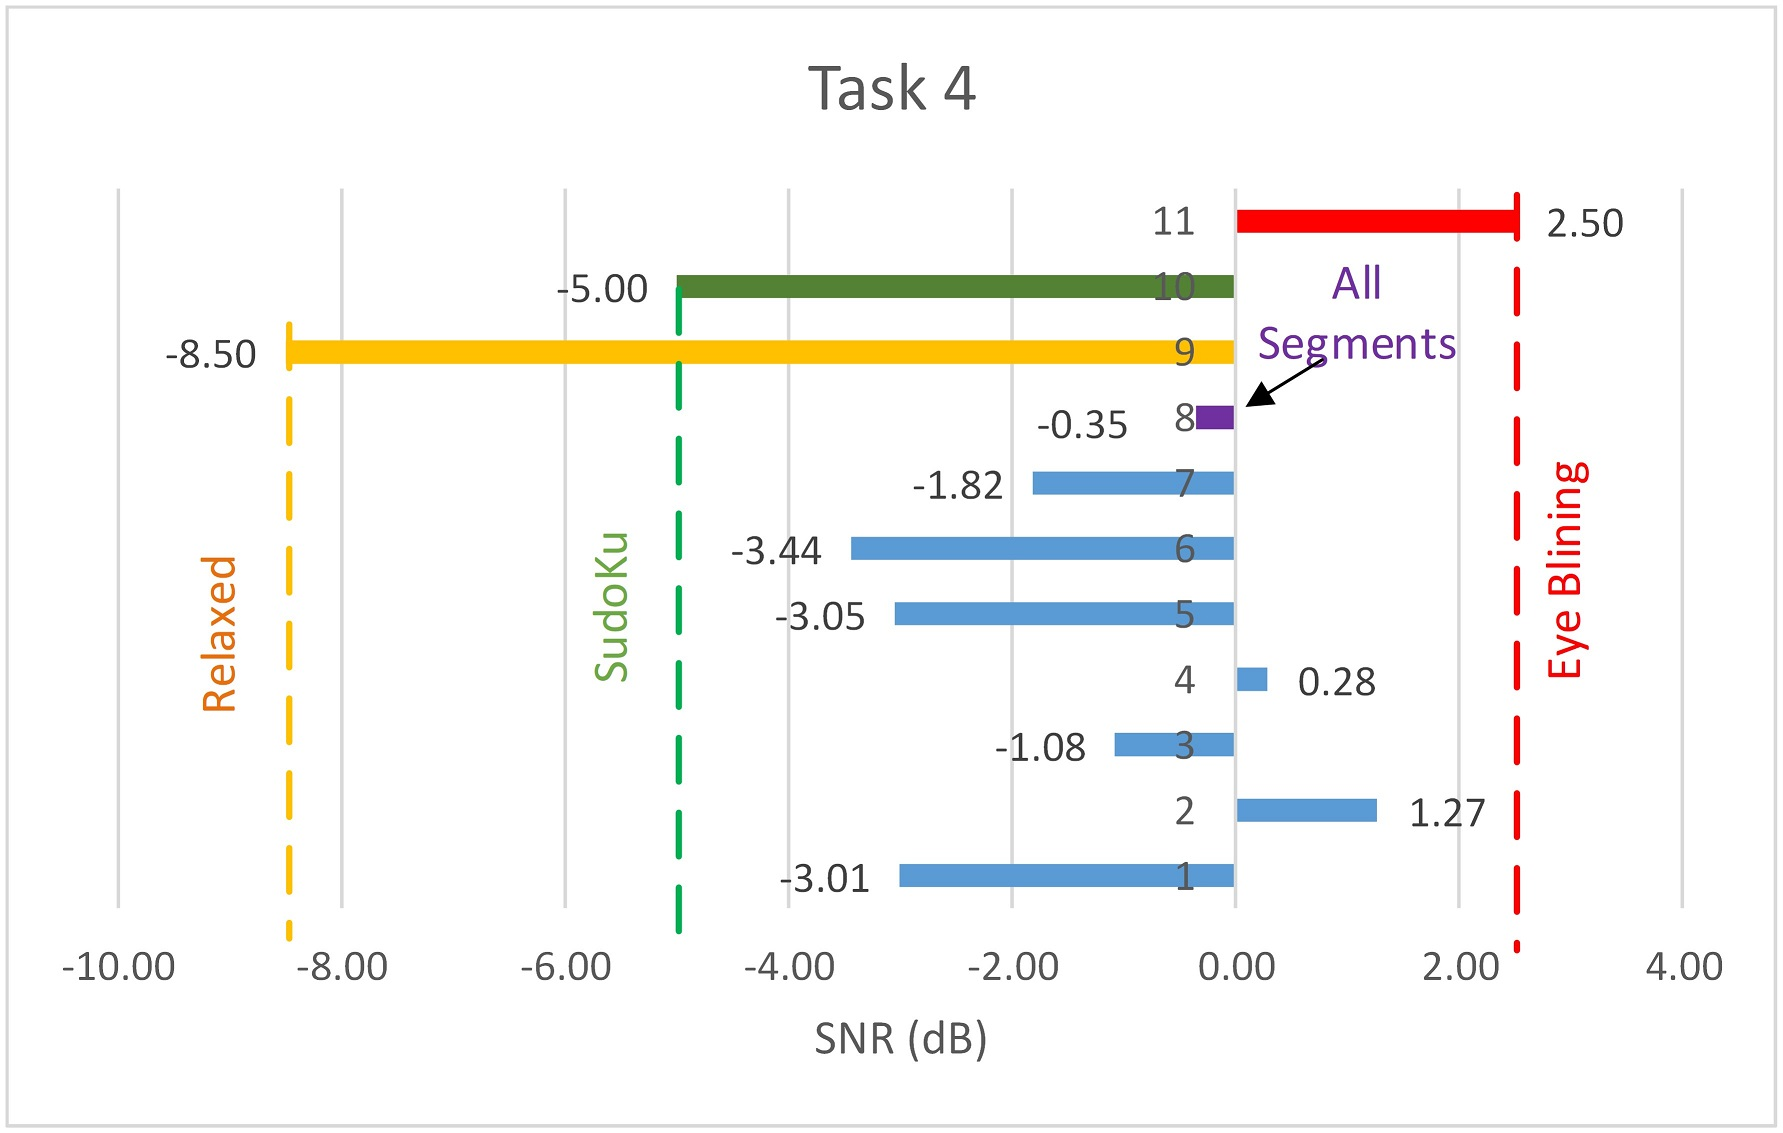
\includegraphics[width=10cm]{Figures/SNRtask4.jpg} 
	\caption{SNR for Task4.} 
	\label{SNR4} 
\end{figure}


\begin{figure}[hbt!]
	\centering
%	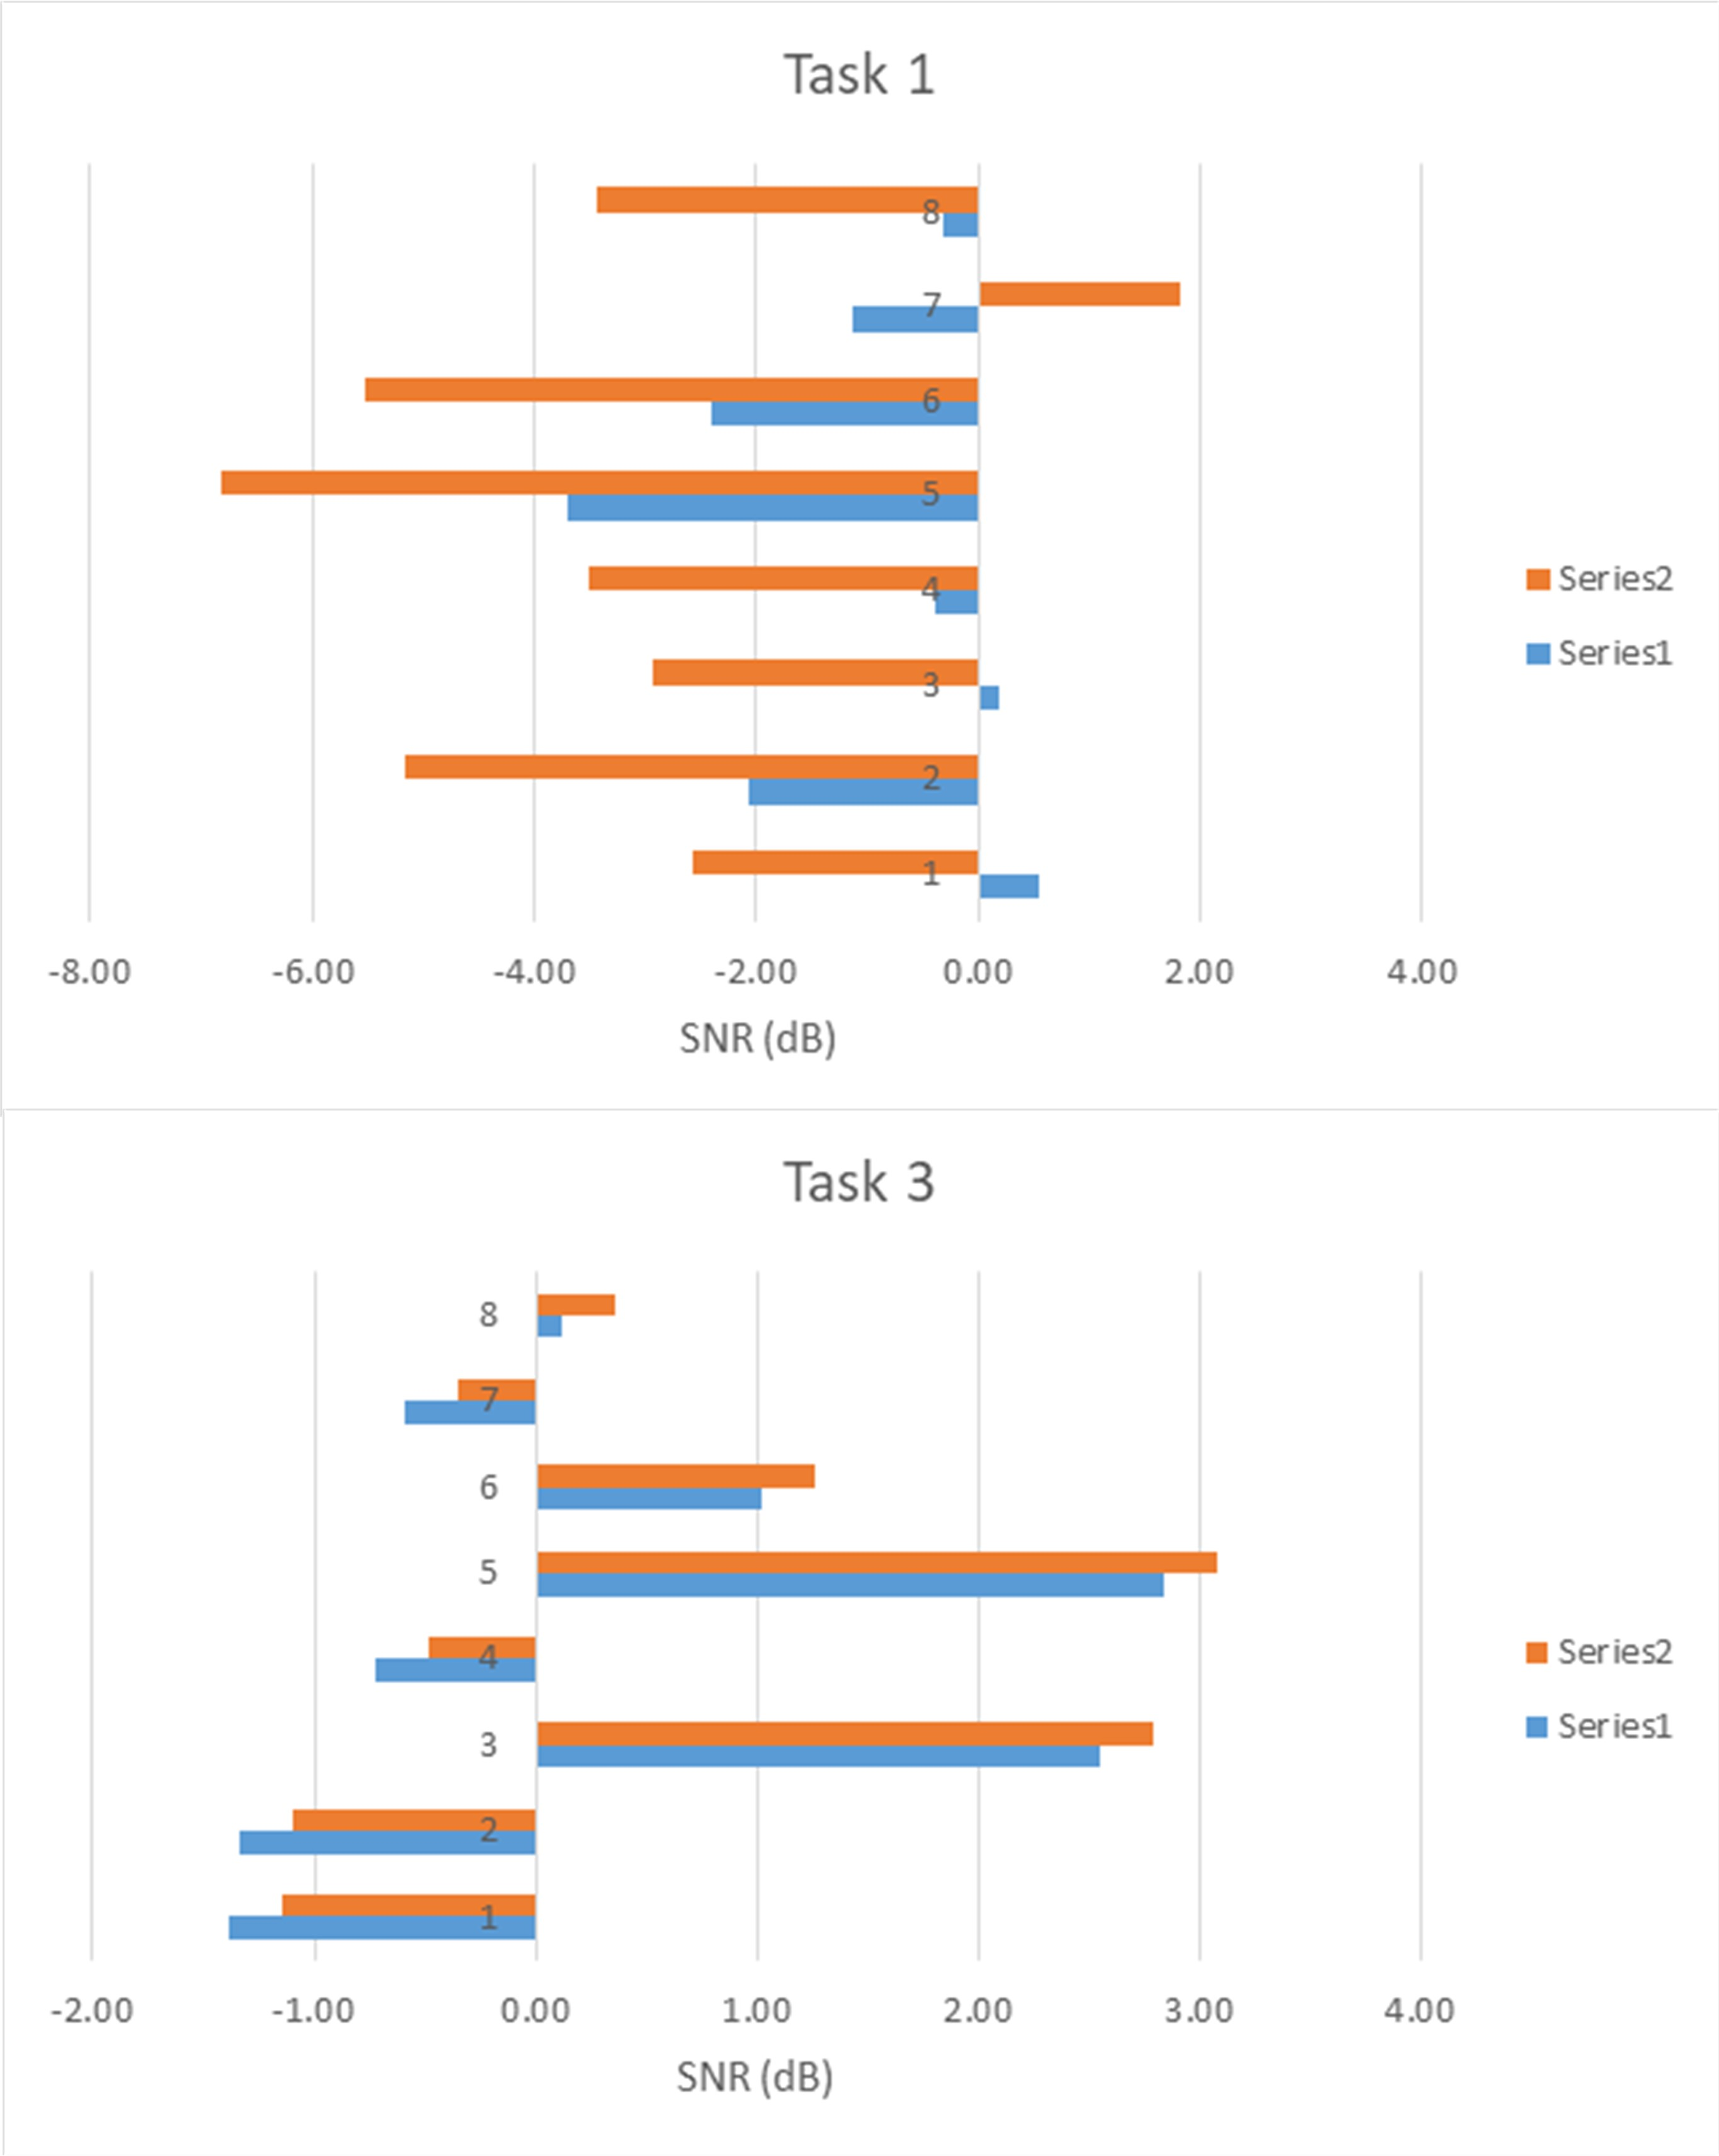
\includegraphics[width=\linewidth]{Figures/SNRchange.jpg} 
	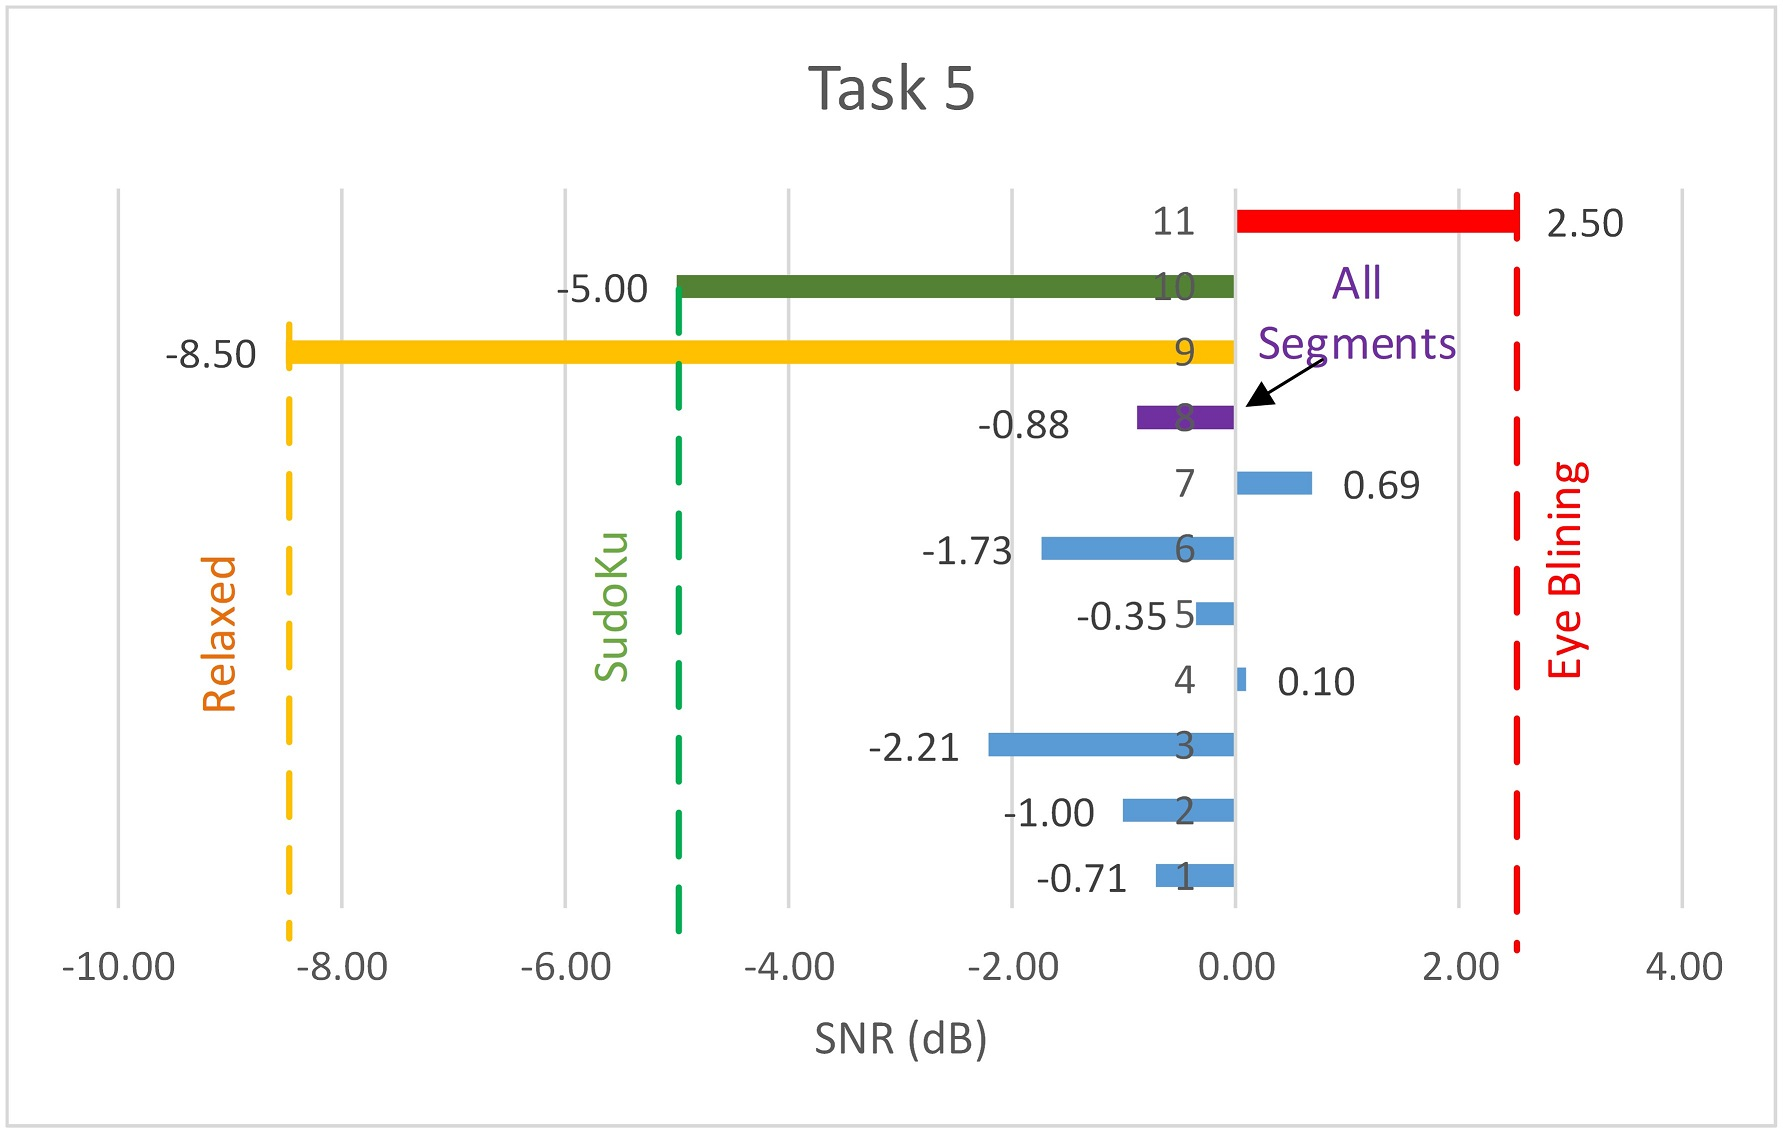
\includegraphics[width=10cm]{Figures/SNRtask5.jpg} 
	\caption{SNR for Task5.} 
	\label{SNR5} 
\end{figure}


\begin{figure}[hbt!]
	\centering
%	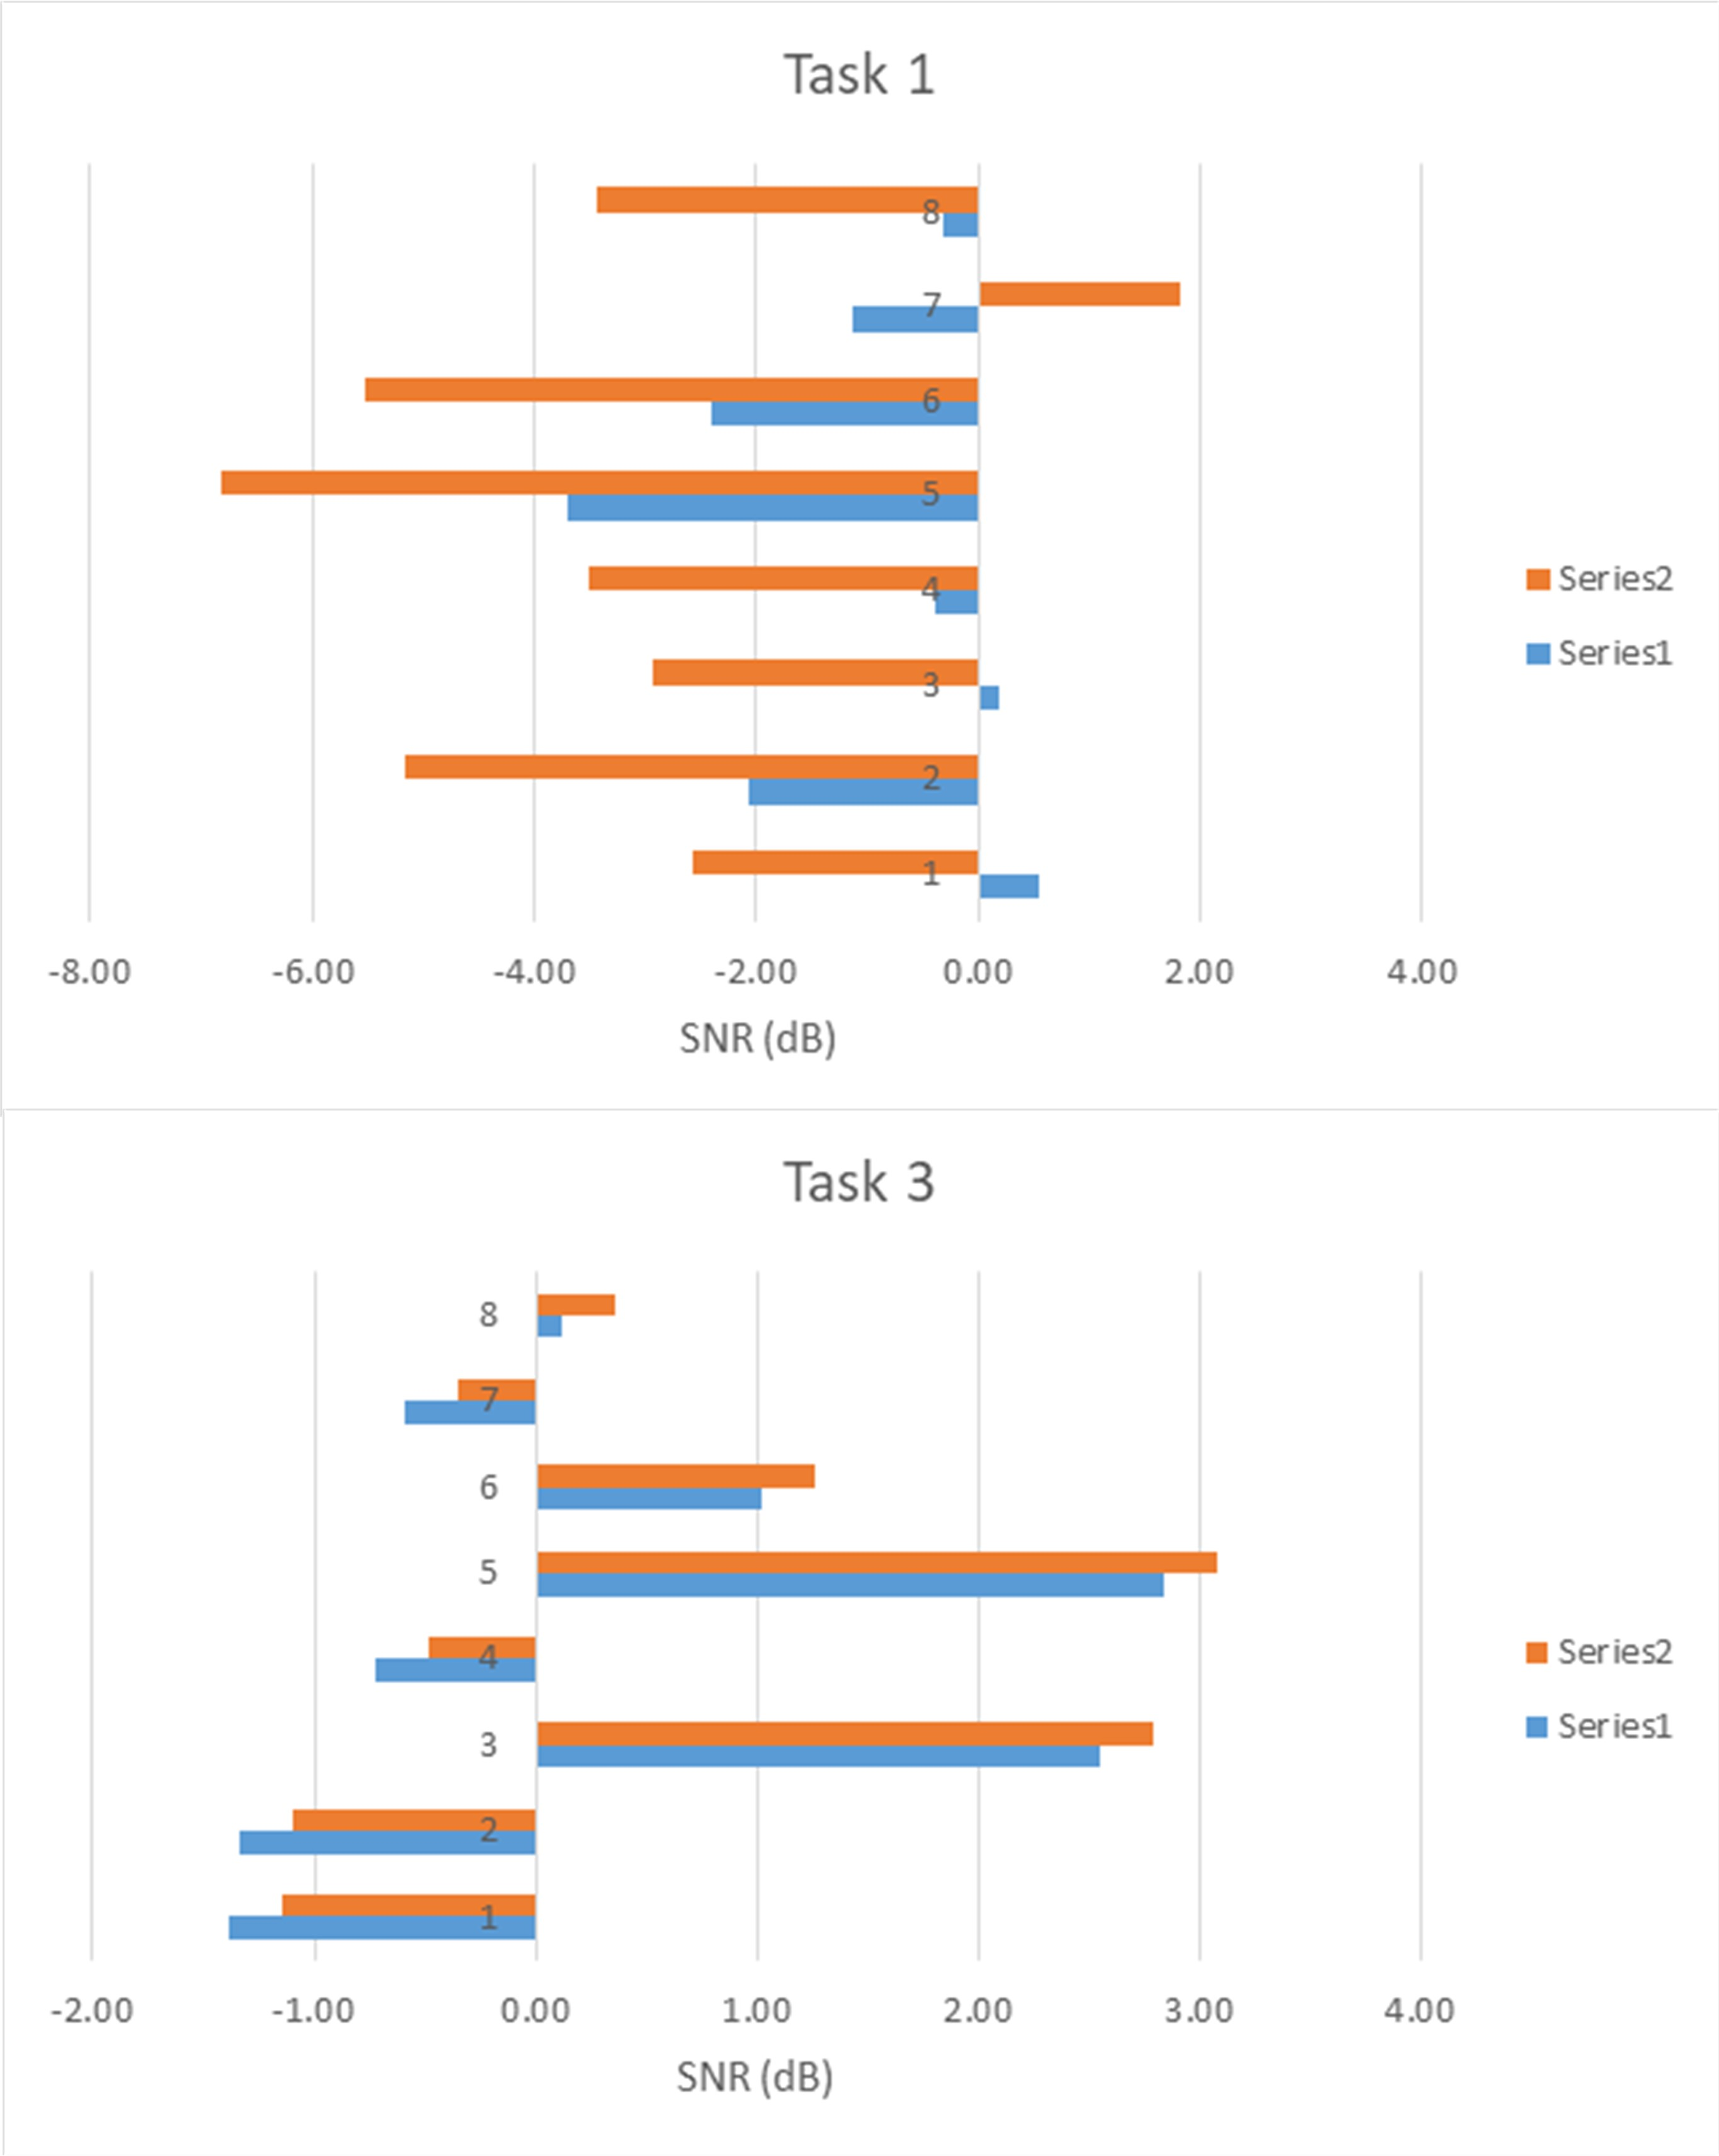
\includegraphics[width=\linewidth]{Figures/SNRchange.jpg} 
	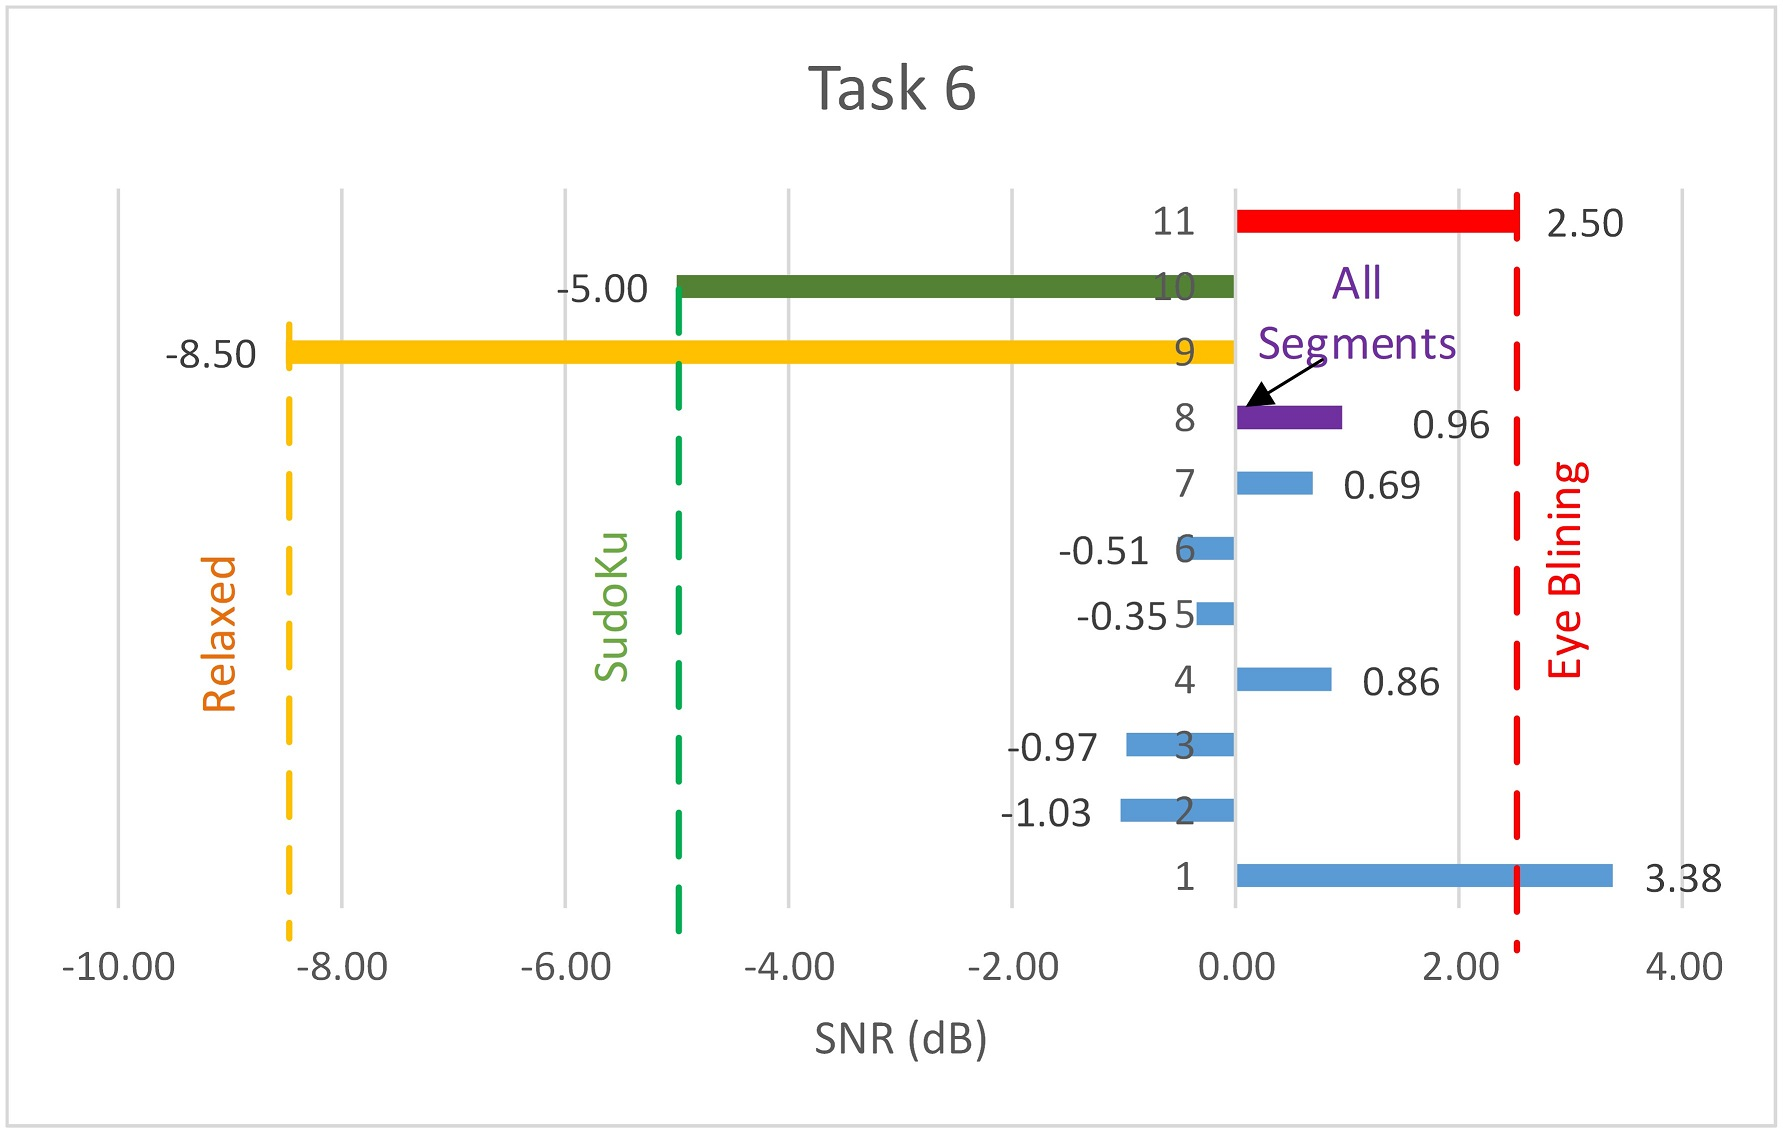
\includegraphics[width=10cm]{Figures/SNRtask6.jpg} 
	\caption{SNR for Task6.} 
	\label{SNR6} 
\end{figure}


\begin{figure}[hbt!]
	\centering
%	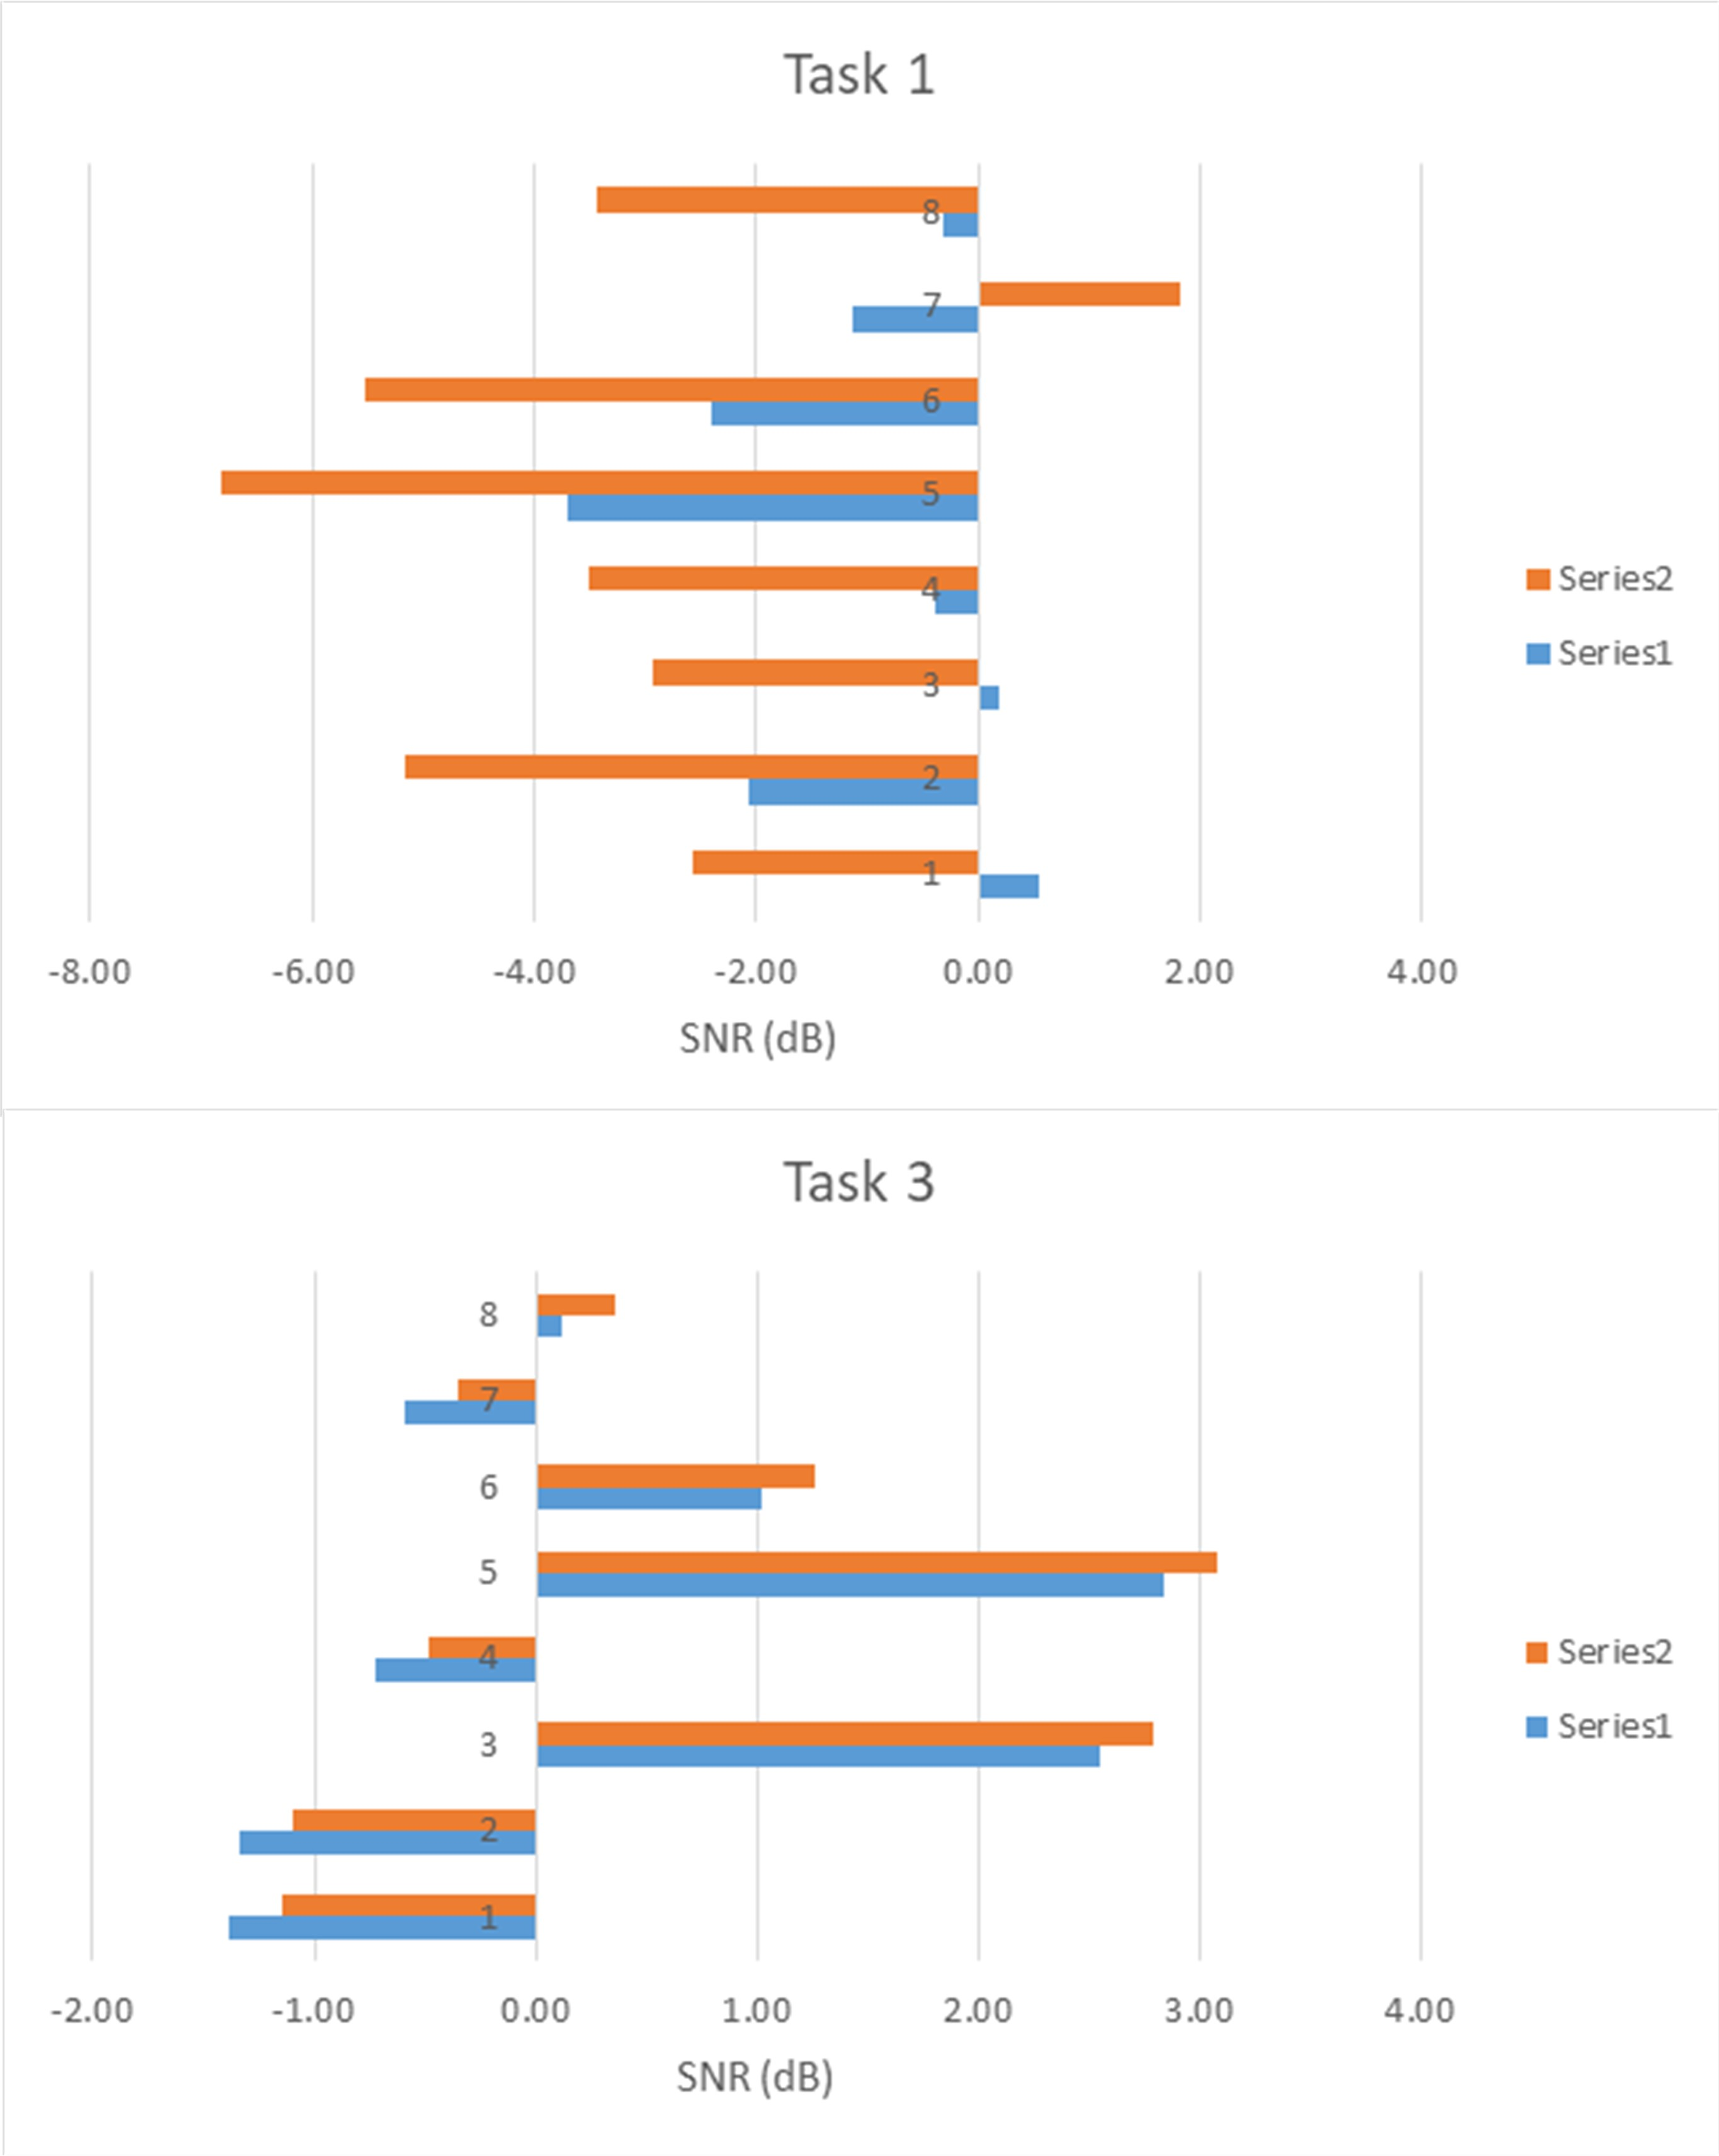
\includegraphics[width=\linewidth]{Figures/SNRchange.jpg} 
	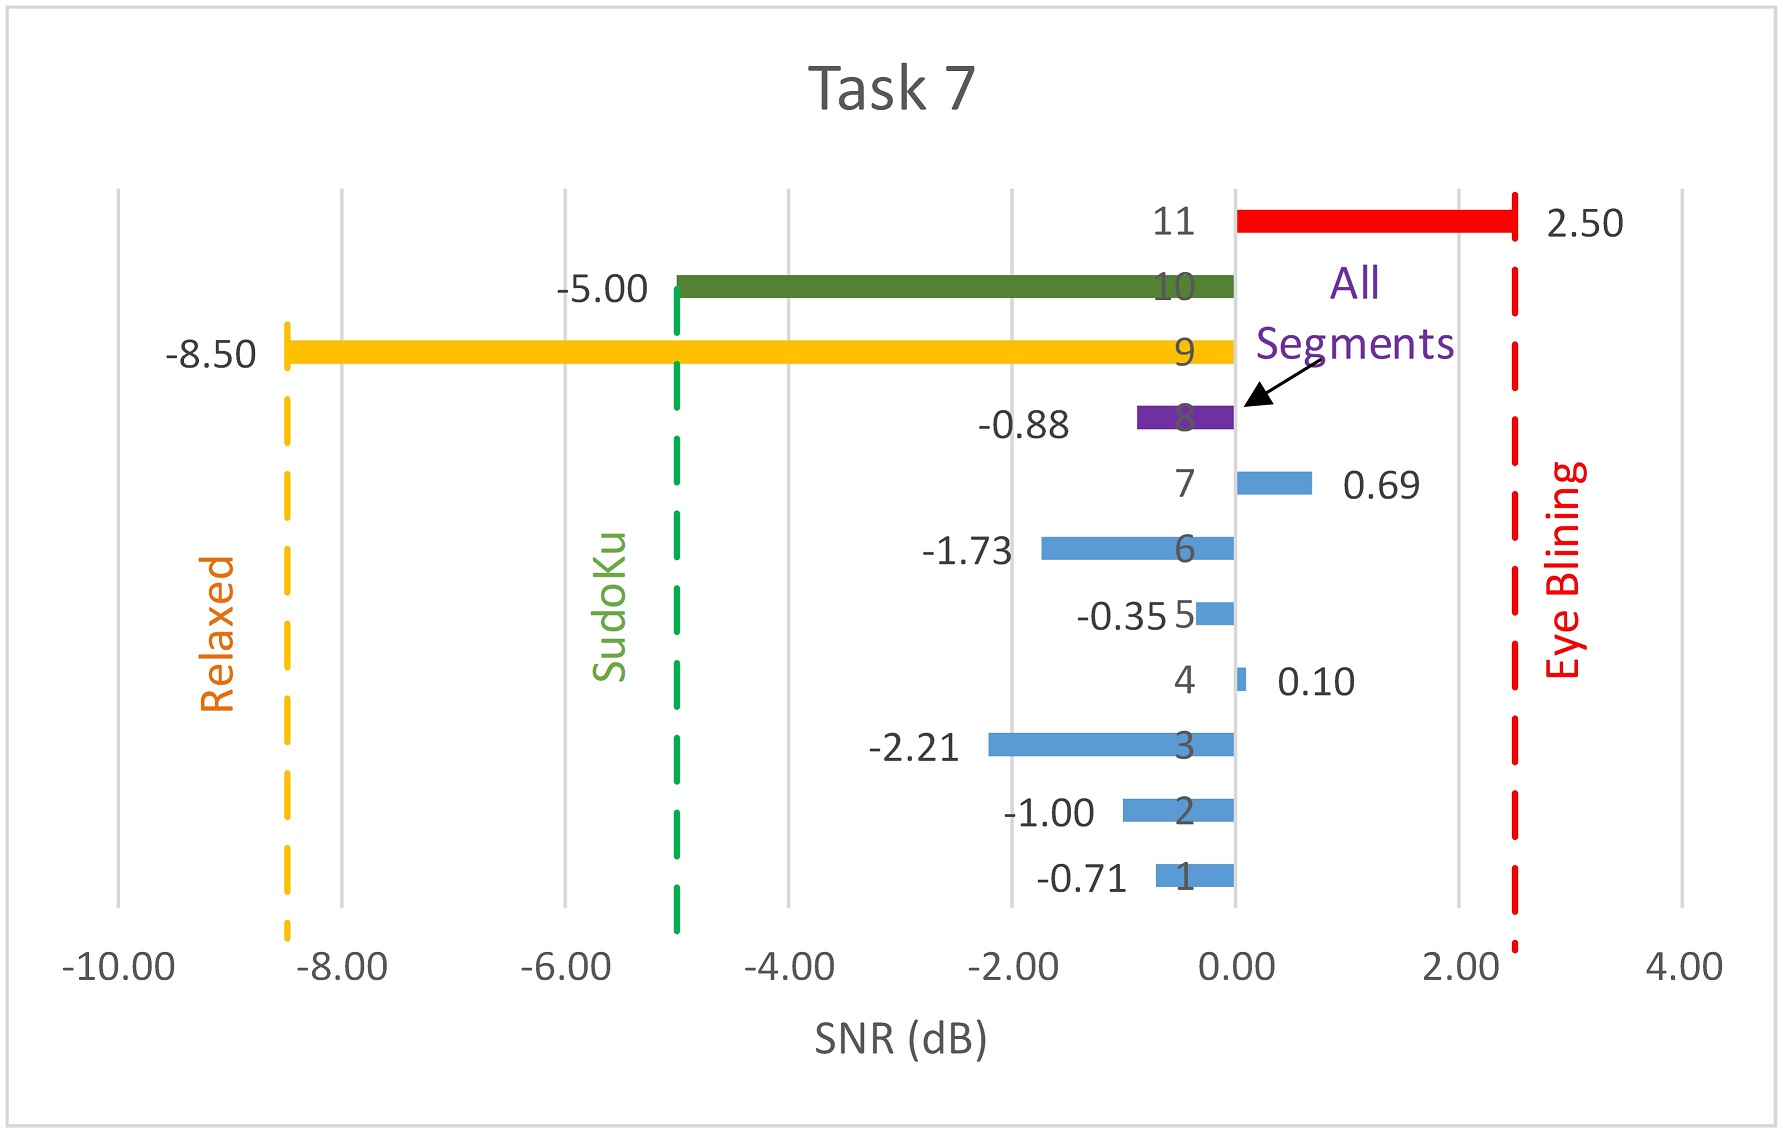
\includegraphics[width=10cm]{Figures/SNRtask7.jpg} 
	\caption{SNR for Task7.} 
	\label{SNR7} 
\end{figure}

From the SNR for all of the experiments it can be seen that the SNR values change between signal segments. For example for the case of Task 7, the SNR is equal to -0.71dB when the EEG recording is examined during the time interval from 4s to 5s (segment 1), while it is +0.69dB during the time interval from 7s to 8s. The worst case for Task7 occurs on the signal segment 3, where the SNR is -2.21dB. Each plot also shows the overall SNR for the Task, which corresponds to the EEG signal from 4s to 8s. The fact that the SNR is not the same between the various signal segments of the task is in accordance with the observation of the alpha band spectrum, where the peak of the 10Hz frequency was varying between signal segments. This variations of the SNR can be justified by the fact that when a person concentrates on performing a specific task, and this effort lasts many seconds, his attention can vary. In other words at some instances his effort is more intensive than in other instances. 

As far as the critical issue on whether the use of EEG signals obtained from a single electrode attached at position Fp1, is concerned, it can be observed that in all tasks and during all segment durations, the SNR achieved is higher than the SNR wall for the ‘relaxed’ and the ‘Sudoku’ case. Unlike the “eye blinking” case, where in almost all cases the SNR achieved is less than the SNR wall.
      
As a general conclusion, based on the EEG recordings available, it can be claimed that the proposed configuration of using EEG from the FP1 position only, can correctly detect the EEG signal and thus determine the intent of the subject. In the case of extreme noise, such as the eye blinking artefacts, once the artefact is detected, the BCI system can ignore the signal segment during the artefact, and thus avoid false detections.  






\newpage
\newpage
\section{\centerline{Conclusions and Future Work}}
\label{sec:conclusions}

\vspace {20pt}

This report presents a study on the ability of a BCI system to detect an EEG signal using a single electrode connected to the Fp1 position. This investigation is concentrated on the alpha band frequencies (8Hz to 12Hz) with special interest on the 10Hz peaks.

One of the main actions taken towards the completion of this work, was the setup of the equipment to be used in order to conduct the experiments and record the EEG data. A number of problems were encountered in the process of setting up the experimental equipment. A consequence of that was a delay in the steps described in the project schedule submitted with the Project Proposal. The first problem was related to the assembly of a cable connecting the amplifier with the data acquisition board. The pin numbers on the amplifier connector given in the schematic diagram were specified wrong. As a consequence of that, the EEG recording system was not functioning, until the problem was identified and fixed. The second issue was related to the incompatibility of the amplifier output voltage with the maximum input voltage of the data acquisition board. The amplifier output voltage swings from -5V to +5V, while the maximum input voltage of the data acquisition board is -1.33V to +1.33V. This incompatibility, in conjunction with the gain of the amplifier resulted in exceeding the maximum input voltage of the analogue to digital converter creating excessive harmonics on the recorded signals. This problem was addressed by changing the gain of the amplifier from 500 to 50.

The methodology designed for this project included the recording of EEG signals from a number of willing persons. The use of people willing to participate as the subject requires a prior approval by the Ethics Committee of the University. An application for the approval of the process has been submitted to the Ethics Committee with a considerable delay due to the hardware problems mentioned above. The approval of this request was not granted till the deadline of the submission of the project report. As a consequence of that, the analysis of the EEG signals was made using EEG data recorded using the author of this report as the only subject.
The recorded EEG signals were investigated with respect of the existence of a peak at the 10Hz frequency and on the calculation of the SNR. To this end, the recorded signals were first filtered to remove the 50Hz mains noise and then filtered again in order to isolate the alpha band frequencies. As far as the 10Hz peak is concerned, it was observed by using the frequency spectrum plots, that the 10Hz was indeed present and that its amplitude can vary according to the motor imagery action of the subject. Other observations on this 10Hz peaks are that (a) these peaks can be shifted to lower or higher frequencies such as 9Hz or 11Hz, and (b) these peaks are not constant during the mental task effort of the subject.
   
The second and main investigation of this project was the calculation of the SNR of the recorded EEG signals, in order to decide whether the proposed BCI setting with a single electrode attached on the Fp1 position can correctly detect the EEG signal. The calculated SNR were then compared with the noise walls determined in a project conducted in 2018.  The calculated SNR were found to be bigger than the SNR walls corresponding to the relaxed SNR wall and the Sudoku solving SNR wall. On the other side, the calculated SNR was in almost all cases smaller than the noise wall of the eye blinking artefact. The conclusion from these observations on the SNR, is that a BCI with a single electrode connected to the Fp1 position can safely decode the EEG signals. However, care must be taken to avoid or reduce the noise due to artefacts.

Future work for the improvement of this work is primarily related to the use of a number of subjects to record EEG signals that will result in more reliable conclusions. A second issue that can improve the accuracy of the results is related to the fact that for the calculation of the SNR, the noise from artefacts was assumed to be zero. This however is not always true, since artefacts can be caused unintentionally. To this end, a de-noising scheme can be included in the methodology in order to remove as much of the artefact noise as possible. 





%----------------------------------------------------------------------------------------
%	BIBLIOGRAPHY
%----------------------------------------------------------------------------------------
\newpage
\section{Bibliography}
\printbibliography%[title={Bibliography}] % Print the bibliography, section title in curly brackets
%\bibliographystyle{plain}

%\bibliography{references,acsac06-refs,costas,extra,ddm,tpds_ddm}
%\bibliography{example}
%----------------------------------------------------------------------------------------

\end{document}
